%% Elsevier CAS double-column template (cas-dc.cls).
%% Target: Knowledge-Based Systems (Elsevier).
%%
%% GENERATED FILE -- do not edit by hand.
%%   Source:    paper/sn-article.tex
%%   Generator: scripts/make_elsevier.py
%% Edit the source and regenerate, or the numbers will drift from
%% artefacts/ and scripts/check_paper_numbers.py will stop protecting them.
%%
%% Build:  pdflatex kbs-article && bibtex kbs-article
%%         && pdflatex kbs-article && pdflatex kbs-article
%%
%% cas-dc.cls, cas-common.sty and the .bst files are NOT redistributed here.
%% Fetch them with:  bash paper-kbs/fetch-template.sh
\documentclass[a4paper,fleqn]{cas-dc}

%% cas-dc.cls loads neither amsmath nor the table packages this manuscript
%% needs. Same list as the Springer build, minus what cas-dc provides.
\usepackage{amsmath}
\usepackage{amssymb}
\usepackage{amsthm}
\usepackage[numbers,sort&compress]{natbib}
\usepackage{microtype}
\usepackage{xurl}
%% cas-dc overlays the keyword box beside the abstract with an intentional
%% zero-width box; silence only that class-internal diagnostic.
\AtBeginEnvironment{Abstract}{\hfuzz=124pt}
\usepackage{multirow}
\usepackage{array}
\usepackage{tabularx}
\usepackage{booktabs}
\usepackage{algorithm}
\usepackage{algpseudocode}
\usepackage{tikz}
\usetikzlibrary{arrows.meta,positioning,fit,backgrounds,calc,shapes.geometric}
\graphicspath{{figures/}}

%% Elsevier uses \tnotemark/\fnmark for title and author notes; hyperref comes
%% from the class, so only the options are set here.
\hypersetup{hypertexnames=false,bookmarksdepth=3}

%% DOUBLE-COLUMN CONSEQUENCE, and the main reason this is not a pure
%% search-and-replace. cas-dc is two-column: the text block is about 84mm per
%% column against roughly 165mm single-column in sn-jnl, so every wide table
%% and every full-width figure must be promoted to a starred float that spans
%% both columns. The generator does that promotion automatically; see
%% `widen_floats` in scripts/make_elsevier.py.

%% Figure 1 renders as live TikZ; set \tikzfigurefalse to fall back to the
%% pre-rendered raster in figures/Fig1.png.
\newif\iftikzfigure
\tikzfiguretrue

%% Figure lettering. Elsevier's artwork instructions ask for legible text at
%% the final printed size; in double column that is a smaller physical width,
%% so the explicit point sizes from the Springer build are kept.
\newcommand{\snFigMain}{\fontsize{9}{10.5}\selectfont}
\newcommand{\snFigSub}{\fontsize{8}{9.5}\selectfont}

\tikzset{
  snstage/.style={
    rectangle, draw=black, line width=0.65pt, fill=white,
    minimum height=18mm, inner sep=3pt, align=center,
    font=\snFigMain, text width=27mm},
  snstagekey/.style={
    rectangle, draw=black, line width=1.0pt, fill=white,
    minimum height=18mm, inner sep=3pt, align=center,
    font=\snFigMain, text width=27mm},
  snfold/.style={
    rectangle, draw=black, dashed, line width=0.5pt, fill=white,
    inner sep=2pt, align=center, font=\snFigSub, text width=19mm},
  snflow/.style={-{Stealth[length=4.5pt,width=3.5pt]}, draw=black,
    line width=0.75pt},
  sndata/.style={-{Stealth[length=4.5pt,width=3.5pt]}, draw=black,
    line width=0.5pt, dashed},
  snout/.style={
    rectangle, draw=black, line width=0.65pt, fill=white,
    minimum height=14mm, inner sep=3pt, align=center,
    font=\snFigMain, text width=34mm},
  sncredit/.style={snout},
  snremoval/.style={snout},
  sninteraction/.style={snout},
  snbranch/.style={draw=black, line width=0.65pt},
  snlbl/.style={font=\snFigSub, inner sep=1.2pt, text=black},
}

%% Float placement. In two columns the queue backs up more easily than in one,
%% so the same remedy as the Springer build applies, and placeins drains the
%% queue at each section boundary.
\renewcommand{\topfraction}{0.9}
\renewcommand{\bottomfraction}{0.8}
\renewcommand{\textfraction}{0.07}
\renewcommand{\floatpagefraction}{0.6}
\renewcommand{\dbltopfraction}{0.9}
\renewcommand{\dblfloatpagefraction}{0.6}
\setcounter{topnumber}{3}
\setcounter{bottomnumber}{2}
\setcounter{totalnumber}{5}
\setcounter{dbltopnumber}{3}
\usepackage{placeins}

\theoremstyle{plain}
\newtheorem{theorem}{Theorem}
\newtheorem{proposition}[theorem]{Proposition}
\newtheorem{lemma}[theorem]{Lemma}

\theoremstyle{definition}
\newtheorem{property}{Property}
\newtheorem{remark}{Remark}

\flushbottom
\emergencystretch=0.75em

\newcommand{\G}{\mathcal{G}}
\newcommand{\Cu}{C_u}
\newcommand{\Ueval}{\mathcal{U}_{\mathrm{eval}}}
\newcommand{\NDCG}{\mathrm{NDCG@10}}
\newcommand{\NDCGat}[1]{\mathrm{NDCG@}#1}
\newcommand{\LOOr}{\mathrm{LOO}_{\mathrm{rank}}}
\newcommand{\LOOe}{\mathrm{LOO}_{\mathrm{e2e}}}
\newcommand{\LOO}{\mathrm{LOO}}

\begin{document}

\let\WriteBookmarks\relax
\def\floatpagepagefraction{1}
\def\textpagefraction{.001}

\shorttitle{Exact-enumeration ranking-stage source attribution}
\shortauthors{M. Louhichi et al.}

\title[mode=title]{SignalShap: Exact-Enumeration Ranking-Stage Attribution of
Sources in Hybrid Recommenders}

\author[1]{Mouad Louhichi}[orcid=0000-0002-6849-230X]
\cormark[1]
\ead{mouad_louhichi@um5.ac.ma}
\credit{Conceptualization, Methodology, Software, Formal analysis,
Investigation, Writing -- original draft, Visualization}

\author[1]{Redwane Nesmaoui}
\ead{redwane.nesmaoui@um5.ac.ma}
\credit{Software, Validation, Data curation, Writing -- review and editing}

\author[1]{Mohamed Lazaar}
\ead{mohamed.lazaar@ensias.um5.ac.ma}
\credit{Supervision, Methodology, Resources, Writing -- review and editing}

\affiliation[1]{organization={National Higher School of Computer Science and
Systems Analysis (ENSIAS), Mohammed V University in Rabat},
  city={Rabat},
  country={Morocco}}

\cortext[1]{Corresponding author.}

\begin{abstract}
Source ablation and Shapley attribution answer different questions: removal
cost and credit allocation. Conflating them can select the wrong decision
instrument.

\emph{SignalShap} formulates source attribution as a five-player cooperative
game over collaborative filtering, content, popularity, recency, and
sequential-order signals. Its payoff is normalised discounted cumulative gain
at rank~10 (NDCG@10) on a fixed, coalition-independent candidate set. Exact
enumeration of all $2^5=32$ coalitions yields Shapley values without
aggregation sampling error, and recovers the known vectors of six analytic
games to an efficiency residual of at most $6.9\times10^{-18}$.

Across three timestamped corpora spanning a $36\times$ density range, two of
the three fitted systems contain a source for which the two rules disagree in
\emph{sign} by a material margin, and this persists across a seed-42
regularisation sweep. Under the evaluated protocol, ranking-stage
leave-one-out agrees more closely than Shapley with observed single-source
end-to-end removal losses on all three corpora: mean rank agreement
$0.96$--$1.00$ against $0.20$--$0.80$ over ten stochastic fits, and the source
with the smallest observed removal loss is identified on $90$--$100\%$ of fits
against $0$--$50\%$.
SignalShap allocates credit in a declared ranking-stage game; leave-one-out
estimates removal effect. We claim credit allocation, not retirement guidance.
Candidate recall is an applicability diagnostic: only MovieLens-1M clears the
declared $0.60$ gate under the frozen primary configuration, Amazon-VG clears
it in the larger-cap sensitivity, and Gowalla is retained as a relative stress
test because training-history masking bounds its recall above by $0.501$.
\end{abstract}

\begin{keywords}
Shapley value \sep
cooperative game theory \sep
hybrid recommender systems \sep
ranking-stage attribution \sep
leave-one-out ablation \sep
two-stage recommendation
\end{keywords}

\maketitle

\section{Introduction}\label{sec:intro}

A production hybrid recommender is an ensemble of architecturally distinct
scorers. A collaborative-filtering component exploits co-occurrence, a content
component exploits item metadata, a popularity component exploits global
frequency, a recency component exploits temporal locality, and a sequential
component exploits order. Two questions then arise: how should the system's
observed value be divided among its sources, and what would happen if one source
were retired? These are credit-allocation and removal-effect questions,
respectively, and they require different instruments. In practice, removal
effects are commonly estimated by \emph{leave-one-out} (LOO) ablation: disable
one source, measure the change in ranking quality, and assign that change to the
source.

LOO is meaningful only relative to the game on which it is computed, and this
paper distinguishes two forms (Section~\ref{sec:background}). End-to-end LOO
removes a source from retrieval and ranking together, so it is the deployment
intervention by definition. Ranking-stage LOO removes the source only from a
fixed-candidate ranker; it is cheaper to compute and, in our experiments,
closely tracks the end-to-end intervention in the evaluated five-source
systems. Dependence among sources does not
invalidate either removal estimand: the intervention cost is well defined for
the interacting system being measured.

LOO is not, however, a complete rule for dividing credit. Hybrid sources often
overlap: for example, implicit-feedback collaborative filtering and popularity
can encode some of the same signal. When two sources are mutually
substitutable, removing either alone may change little, assigning both
near-zero conditional value even though their shared capability contributes to
the system. A credit-allocation rule must also consider coalitions in which no
substitute is available. Neither estimand dominates; they answer different
questions, and this paper measures where they diverge.

Cooperative game theory provides such an allocation rule. The Shapley
value~\citep{shapley1953} is the unique credit assignment satisfying
efficiency, symmetry, null-player, and additivity, and it evaluates each player
against \emph{every} coalition rather than only against the grand coalition.
Its adoption in machine learning has been broad~\citep{lundberg2017,
covert2021explaining}, most commonly at the granularity of \emph{input
features}, though component-level, neuron-level and data-level games also
appear (Section~\ref{sec:related}). Here the players are \emph{architectural
sources}, and the payoff is a ranking metric.

Figure~\ref{fig:workflow} summarises the pipeline. Moving from hundreds of
features to five sources provides two practical advantages. First, generic
model-agnostic feature Shapley is usually approximated because its coalition
lattice is intractable; methods such as KernelSHAP therefore sample and inherit
estimator variance, although exact algorithms exist for particular model
classes, notably trees~\citep{lundberg2020}. Five sources produce only
$2^5=32$ coalitions, and each source has $2^4=16$ marginal contributions. We
evaluate the complete game by exhaustive enumeration, so the attribution
introduces no aggregation sampling error.
Second, the small player set improves \emph{verifiability}: we can construct
games and interventions whose attributions must satisfy known constraints, then
test whether the implementation does so. Section~\ref{sec:recovery} applies
this strategy to analytic and real fitted games.

\begin{figure*}[tp]
\centering
\iftikzfigure
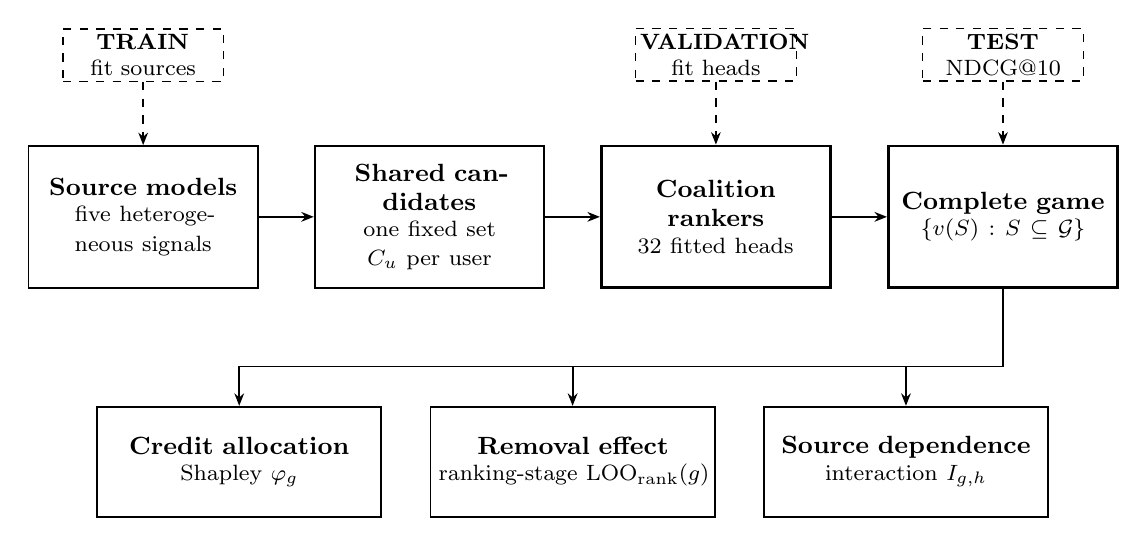
\begin{tikzpicture}[node distance=7mm]
\node[snstage] (src)
  {\textbf{Source models}\\[-1pt]
   {\snFigSub five heterogeneous signals}};
\node[snstage, right=of src] (cand)
  {\textbf{Shared candidates}\\[-1pt]
   {\snFigSub one fixed set $\Cu$ per user}};
\node[snstagekey, right=of cand] (heads)
  {\textbf{Coalition rankers}\\[-1pt]
   {\snFigSub $32$ fitted heads}};
\node[snstagekey, right=of heads] (game)
  {\textbf{Complete game}\\[-1pt]
   {\snFigSub $\{v(S):S\subseteq\G\}$}};

\draw[snflow] (src) -- (cand);
\draw[snflow] (cand) -- (heads);
\draw[snflow] (heads) -- (game);

\node[snfold, above=8mm of src] (train)
  {\textbf{TRAIN}\\{\snFigSub fit sources}};
\node[snfold, above=8mm of heads] (val)
  {\textbf{VALIDATION}\\{\snFigSub fit heads}};
\node[snfold, above=8mm of game] (test)
  {\textbf{TEST}\\{\snFigSub NDCG@10}};
\draw[sndata] (train) -- (src);
\draw[sndata] (val) -- (heads);
\draw[sndata] (test) -- (game);

\coordinate (outmid) at ($(cand)!0.5!(heads)$);
\node[snremoval, below=24mm of outmid] (removal)
  {\textbf{Removal effect}\\[-1pt]
   {\snFigSub ranking-stage $\LOOr(g)$}};
\node[sncredit, left=6mm of removal] (credit)
  {\textbf{Credit allocation}\\[-1pt]
   {\snFigSub Shapley $\varphi_g$}};
\node[sninteraction, right=6mm of removal] (interaction)
  {\textbf{Source dependence}\\[-1pt]
   {\snFigSub interaction $I_{g,h}$}};

\coordinate (busleft) at ($(credit.north)+(0,5mm)$);
\coordinate (busmid) at ($(removal.north)+(0,5mm)$);
\coordinate (busright) at ($(interaction.north)+(0,5mm)$);
\draw[snbranch] (game.south) |- (busmid);
\draw[snbranch] (busleft) -- (busright);
\draw[snflow] (busleft) -- (credit.north);
\draw[snflow] (busmid) -- (removal.north);
\draw[snflow] (busright) -- (interaction.north);

\end{tikzpicture}%
\else
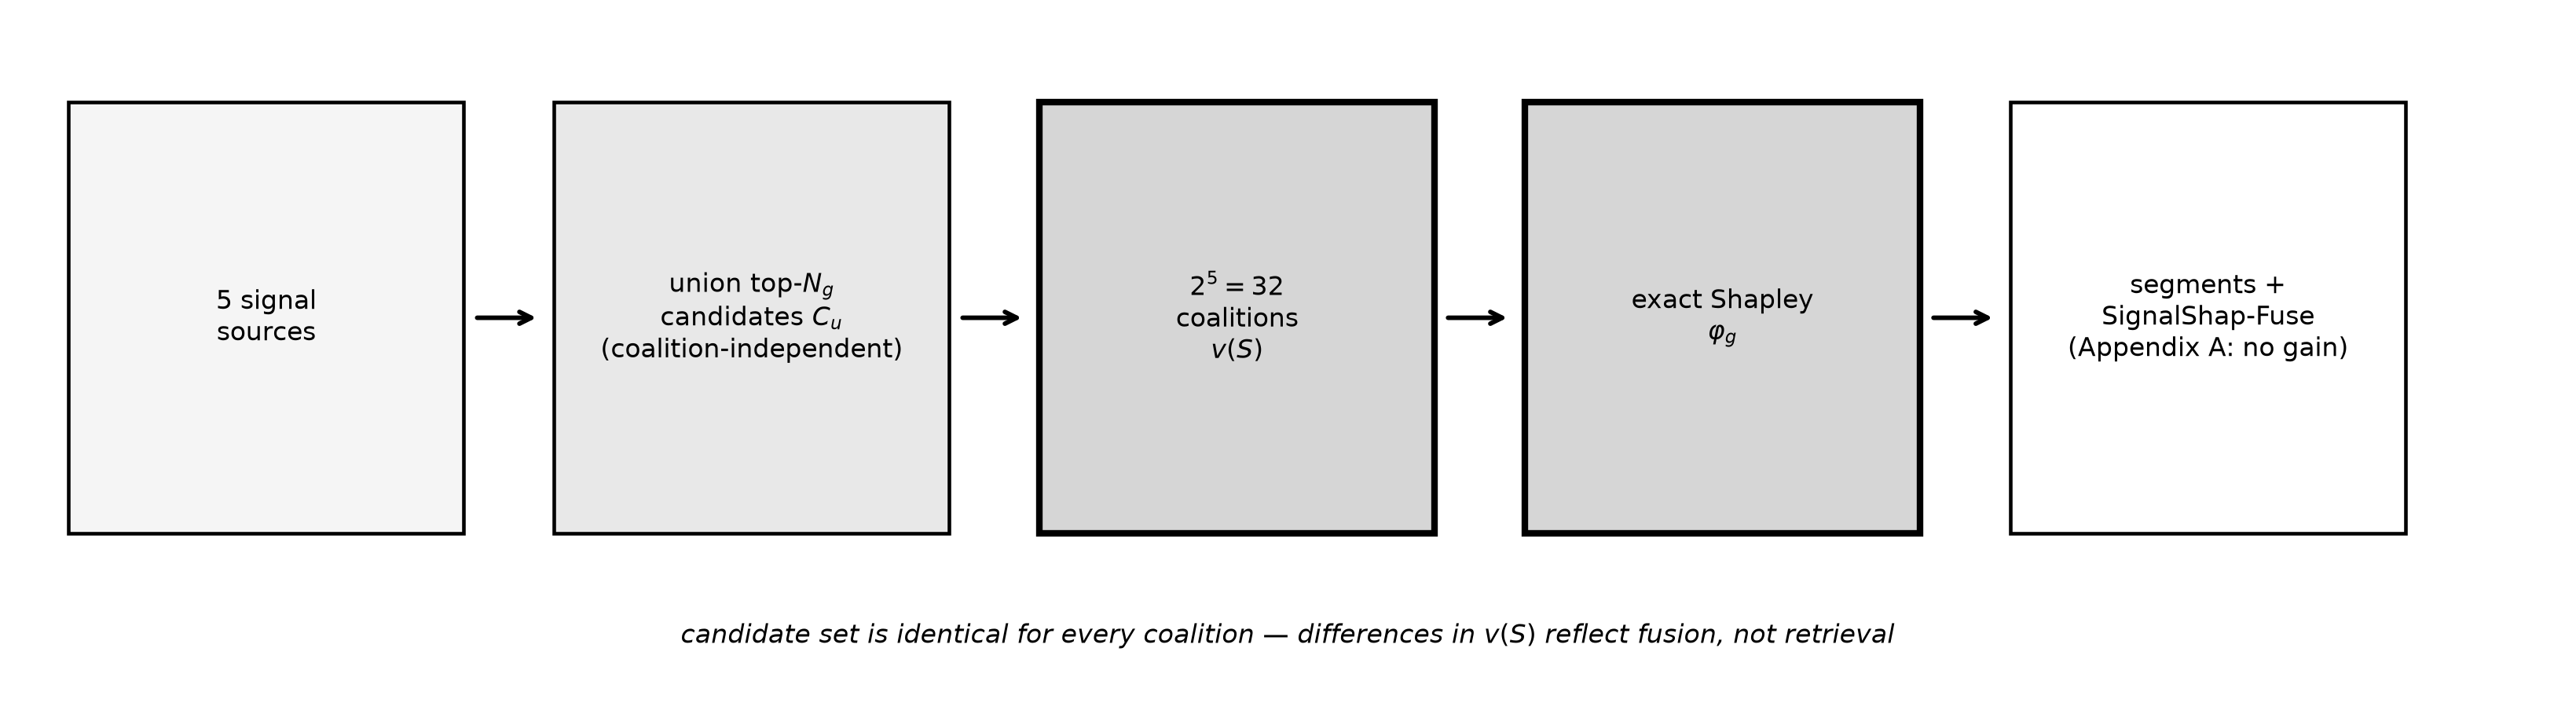
\includegraphics[width=\linewidth]{Fig1.png}
\fi
\caption{SignalShap workflow from source fitting and shared candidates to
exact-game diagnostics.}
\label{fig:workflow}
\end{figure*}

\subsection{Contributions}

\begin{itemize}
\item \textbf{C1.} A precisely declared ranking-stage cooperative game over
      heterogeneous recommender sources, with a coalition-independent candidate
      set that makes $v(S)$ comparable across coalitions, a per-user
      formulation, and exact enumeration for small source sets
      (Section~\ref{sec:game}).
\item \textbf{C2.} A formal characterisation of source allocation under
      redundancy: efficiency and per-user decomposition, a counterexample
      showing the redundancy--positivity property is \textbf{false} without
      monotonicity, a corrected two-sided $\varepsilon$-substitutability
      result, and the observation that Shapley credit is \emph{not} conserved
      under replication (Section~\ref{sec:theory}).
\item \textbf{C3.} An implementation-verification protocol combining
      analytic games with known Shapley vectors, controlled duplicate
      injection, and efficiency, null-player, and additivity diagnostics
      (Sections~\ref{sec:recovery} and~\ref{sec:validating}). Together, these
      checks establish that the aggregation is implemented correctly, a
      precondition for interpreting the resulting attributions.
\item \textbf{C4 (primary).} A conditional empirical comparison of three games
      (refitted-head ranking-stage, fixed-head ranking-stage, and end-to-end
      retrieval) and two attribution rules, showing that Shapley allocation and
      leave-one-out removal cost answer \emph{different questions}. Two of the
      three systems contain a source for which the rules disagree in sign by a
      material margin throughout a labelled seed-42 regularisation sweep. Over
      ten stochastic fits of each fixed corpus, ranking-stage leave-one-out has
      higher agreement with observed end-to-end retirement losses than Shapley
      (mean rank agreement
      $0.96$--$1.00$ against $0.20$--$0.80$) and identifies the
      source with the smallest observed removal loss on $90$--$100\%$ of seeds against
      $0$--$50\%$ (Wilson intervals in Table~\ref{tab:retire-seeds}). We pair this with
      candidate recall as a necessary applicability diagnostic under a
      declared $0.60$ reporting gate, restricting absolute comparisons where
      that gate fails (Sections~\ref{sec:results} and~\ref{sec:estimands}).
\end{itemize}

\paragraph{What this paper does not claim}
We do not claim that attribution-derived fusion weights improve ranking
quality: their observed difference from a globally tuned head is practically
negligible under the reported protocol, and we report that negative result in
Appendix~\ref{app:fusion} rather than as a contribution. We make no
state-of-the-art claim against LightGCN or SASRec; those models appear as
contextual references only, and received smaller tuning budgets than a
performance comparison would require. Nor do we claim that the sign of an
attribution prescribes retaining or removing a source;
Section~\ref{sec:estimands} shows that it does not.

\subsection{Research questions}

\begin{description}
\item[RQ1] Does a fixed-candidate, coalition-independent cooperative game over
  architectural sources admit an exact additive decomposition of its value
  relative to baseline, and does the implementation satisfy known Shapley
  constraints on analytic and real fitted games?
\item[RQ2] Does source-level Shapley attribution differ materially from
  leave-one-out ablation, and is the difference associated with source-score
  overlap or negative pairwise interaction under the declared game?
\item[RQ3] How do attributions change across refitted-head ranking-stage,
  fixed-head ranking-stage, and end-to-end games, and does ranking-stage LOO or
  Shapley better predict observed end-to-end retirement cost?
\end{description}

\paragraph{What is not in this paper} Graph-neural or Transformer players;
causal attribution; online or counterfactual evaluation. All attribution is
\emph{within} a declared game. The primary analysis uses a fixed candidate set;
the end-to-end variant is included only to compare estimands and evaluate the
retirement decision.

\paragraph{Roadmap} Section~\ref{sec:related} reviews component-level and
ranking-specific attribution. Section~\ref{sec:background}
collects the cooperative-game definitions we rely on. Section~\ref{sec:game}
defines the game, Section~\ref{sec:algorithm} gives the algorithm and its cost,
and Section~\ref{sec:theory} the formal properties, including a counterexample
showing that redundancy alone does not guarantee positive credit.
Sections~\ref{sec:setup}--\ref{sec:preconditions} describe the corpora and the
preconditions that govern interpretation of the subsequent results.
Sections~\ref{sec:recovery}--\ref{sec:validating} validate the implementation
against constraints known in advance. Section~\ref{sec:results} reports the
attributions, Section~\ref{sec:estimands} compares estimands and reports the
retirement result, and Sections~\ref{sec:discussion}--\ref{sec:threats}
discuss scope and threats. Appendix~\ref{app:fusion} reports a negative
result.

\section{Literature review}

\subsection{Related work}\label{sec:related}

\paragraph{Shapley values in machine learning}
SHAP~\citep{lundberg2017} unified additive feature attribution; extensions
cover trees~\citep{lundberg2020}, data valuation~\citep{ghorbani2019}, and
federated contribution~\citep{wang2020federated}.
Surveys~\citep{covert2021explaining, rozemberczki2022shapley} note that
model-agnostic estimators commonly sample, because the coalition lattice is
exponential in the number of players, with exact procedures available for
structured model classes. Our setting sidesteps this: five players,
32 coalitions, exact enumeration.

\paragraph{Feature-level XAI versus source-level attribution}
SHAP, LIME~\citep{ribeiro2016}, and Integrated
Gradients~\citep{sundararajan2017} answer ``which input features moved this
prediction?''. We answer ``which architectural component earned the system's
ranking quality?''. The unit of attribution differs, the payoff is a ranking
metric rather than a scalar output, and the actionable decision differs: ours is the allocation of system value across subsystems.

\paragraph{Attribution to model components and to performance}
Closer to our unit of analysis than feature-level XAI is work attributing
behaviour to \emph{model components} rather than inputs. Neuron
Shapley~\citep{ghorbani2020neuron} treats individual neurons as players with a
performance payoff, and ensemble games~\citep{rozemberczki2021ensemble} treat
whole classifiers as players and allocate ensemble accuracy among them. This is the closest structural precedent for what we do, since both take trained models as
players and a performance metric as the characteristic function. Related work
attributes changes in \emph{performance} rather than individual
predictions~\citep{zhang2023performance,shah2024coar}. Component-level
valuation therefore provides a direct precedent; this paper extends that unit
of analysis to architectural sources in a ranking system.

The closest recent comparison to our allocation--removal distinction comes
from ensemble forecasting: Kim et al.~\citep{kim2026forecast} compare
leave-one-model-out importance with an all-subsets Shapley measure and relate
their disagreement to overlap in model errors. Bell et al.~\citep{bell2024lsspa}
develop efficient Shapley performance attribution for least-squares models.
Thus neither component-level performance attribution nor the contrast with a
grand-coalition marginal is new by itself. Our narrower contribution is the
fixed-candidate ranking game and its evaluation in a two-stage recommender.

\paragraph{Shapley beyond supervised prediction}
Shapley attribution has also been applied to unsupervised settings, where the
absence of labels removes the natural payoff that classification or regression
supplies. Our own earlier work~\citep{louhichi2025gametheory} attributes
cluster structure to input features by pairing approximated Shapley values with
multi-level clustering. That work shares this paper's premise, that a cooperative game is a defensible way to divide credit in a model whose internals resist inspection, but differs on every axis that matters here: the players
are input features rather than trained source models, the payoff is cluster
quality rather than ranking utility, and the values are approximated rather
than enumerated exactly. The present paper moves the unit of analysis from
features to architectural components, which is what makes exact enumeration
affordable and what makes the retirement question meaningful in the first
place: one can switch off a recommender source, but not a feature of a
clustering.

\paragraph{Shapley for ranking}
A recent line develops Shapley attribution specifically for ranked outputs.
RankSHAP~\citep{chowdhury2025rankshap} axiomatises feature attribution for
learning-to-rank~\citep{burges2005learning} and evaluates against ranking metrics;
RankingSHAP~\citep{heuss2025rankingshap} gives a listwise formulation;
ShaRP~\citep{pliatsika2025sharp} defines games for score, rank, top-$k$, and
pairwise-preference outcomes. Within recommendation, triplet
importance~\citep{he2024triplet} values training triplets by ranking utility.
All of these take \emph{features} or \emph{training data} as players and
approximate the value by sampling. SignalShap differs on both axes: the players
are architectural source models, and with five players the value is computed by
exhaustive enumeration rather than estimated. The distinguishing design choice
is the coalition-independent candidate set with a coalition-refitted fusion
head, which makes coalition values comparable across a subset lattice in a
two-stage retrieval-then-rank architecture, a construction these works do not require because their players do not affect retrieval.

\paragraph{Which Shapley, and which game}
Shapley uniqueness holds \emph{once a game is fixed}; it does not select the
game. Sundararajan and Najmi~\citep{sundararajan2020many} show that plausible
operationalisations differ materially, which is why we state our candidate
construction, coalition head, and baseline explicitly and treat them as
declared modelling choices rather than as the canonical formulation.
Alternative cooperative values (Banzhaf and other semivalues~\citep{karczmarz2022banzhaf}) and interaction-aware extensions
such as the Shapley interaction index~\citep{grabisch1999interaction} and the
Shapley--Taylor index~\citep{sundararajan2020shapleytaylor} are natural
comparators, as are faithful~\citep{tsai2023faithshap} and
regression-based~\citep{fumagalli2024kernelshapiq} interaction formulations.
Because every game we fit is non-monotone, recent work on negative interactions
in non-convex games~\citep{chang2025negative} is also directly relevant. Because redundancy between sources is central to our setting we
evaluate Banzhaf, two binomial semivalues, and the Grabisch--Roubens interaction
index rather than deferring them (Section~\ref{sec:alternatives}); we do not
compute Shapley--Taylor, and Section~\ref{sec:alternatives} explains why the
distinction matters.
Replication sensitivity of Shapley allocations~\citep{han2022replication} is
directly relevant to our duplicate-injection design and is discussed in
Section~\ref{sec:recovery}.

\paragraph{Why not a graph or neural explainer}
A parallel line explains \emph{neural} recommenders by attributing to graph
structure: GNNExplainer~\citep{ying2019gnnexplainer} and
PGExplainer~\citep{luo2020pgexplainer} learn edge and feature masks,
GraphSVX~\citep{duval2021graphsvx} gives those masks a Shapley reading, and
SubgraphX~\citep{yuan2021subgraphx} searches connected subgraphs with a
Shapley scoring function. These are not comparators for the present study, and
the reason is the unit of attribution rather than a judgement of quality. They
attribute to \emph{entities inside one differentiable model}, nodes, edges or
input features, and most require gradients or a message-passing structure. Our
players are five \emph{architecturally distinct scorers}, only one of which is
even a latent-factor model, and the payoff is a ranking metric over a
retrieved candidate set rather than a differentiable output. There is no shared
graph to mask and no gradient to integrate. The comparators that do apply at
this granularity are other cooperative values over the same game, which is why
we evaluate Banzhaf, two binomial semivalues, permutation importance and
forward selection rather than a graph explainer. Extending the game so that a
graph-neural component is one of the players is the natural bridge, and we
name it as future work rather than claim it here.

\paragraph{Offline recommender evaluation and exposure bias}
Logged recommendation data reflect both user choice and earlier exposure
policies. Counterfactual risk minimisation addresses learning from logged bandit
feedback~\citep{swaminathan2015counterfactual}, while propensity-based
recommendation evaluation treats recommendations as interventions and corrects
selection bias~\citep{schnabel2016treatments}. SignalShap does neither: it
attributes an offline metric under the observed-data protocol. The temporal and
exposure limitations of that choice are measured in Section~\ref{sec:setup} and
bounded in Section~\ref{sec:threats}; no causal or off-policy claim is made.

\paragraph{Hybrid recommenders and ablation practice}
Burke's taxonomy~\citep{burke2002hybrid} classifies hybridisation strategies;
weighted and feature-combination hybrids dominate practice. Evaluation of
component worth is predominantly by
ablation~\citep{zangerle2022evaluating}. Recent recommender XAI
work~\citep{zhang2020explainable} explains \emph{recommendations}, not
\emph{architectures}.

\subsection{Background}\label{sec:background}

We collect the definitions the rest of the paper assumes. Readers familiar with
cooperative games may skip to Section~\ref{sec:game}.

\paragraph{Cooperative games and the Shapley value}
A transferable-utility game is a pair $(\G, v)$ with a finite player set $\G$,
$n = |\G|$, and a characteristic function $v : 2^{\G} \to \mathbb{R}$ giving the
value each coalition achieves on its own. The Shapley
value~\citep{shapley1953} allocates $v(\G)$ among the players by averaging each
player's marginal contribution over all orderings, and is the unique allocation
satisfying efficiency, symmetry, null player, and additivity. Nothing in the
axioms selects $v$: uniqueness is conditional on a game the modeller declares,
which is why Section~\ref{sec:game} states ours explicitly and
Section~\ref{sec:estimands} compares alternatives.

For completeness, efficiency requires
$\sum_g\varphi_g=v(\G)-v(\varnothing)$; symmetry assigns equal values to
players with identical marginal contributions; the null-player axiom assigns
zero to a player whose marginal contribution is always zero; and additivity
requires $\varphi(v_1+v_2)=\varphi(v_1)+\varphi(v_2)$.

\paragraph{Semivalues}
Relaxing efficiency yields a family of \emph{semivalues}, each averaging
marginal contributions under a predeclared distribution $p_k$ over the size $k$
of the predecessor coalition:
%
\begin{equation}
\begin{aligned}
\psi_g(v)
  &= \sum_{k=0}^{n-1} \frac{p_k}{\binom{n-1}{k}}
     \sum_{\substack{S \subseteq \G \setminus \{g\} \\ |S| = k}}
     \bigl[v(S \cup \{g\}) - v(S)\bigr],\\
\sum_{k=0}^{n-1} p_k &= 1 .
\end{aligned}
\label{eq:semivalue}
\end{equation}
Shapley is the member with
$p_k = 1/n$ for every $k$: its permutation weight
$|S|!\,(n-|S|-1)!/n! = 1/\bigl(n\binom{n-1}{|S|}\bigr)$ places mass $1/n$ on
each size and spreads it evenly over the $\binom{n-1}{k}$ coalitions of that
size. A ``size-uniform semivalue'' is therefore not an alternative to Shapley;
it is Shapley. Banzhaf is the member with
$p_k = \binom{n-1}{k}2^{-(n-1)}$, which weights all $2^{n-1}$ coalitions
equally and does not satisfy efficiency. The genuinely distinct comparators we
use are the binomial semivalues $p_k = \binom{n-1}{k}q^k(1-q)^{n-1-k}$ at
$q = 0.25$ and $q = 0.75$, which tilt the weight towards small or large
predecessor coalitions respectively. Equation~(\ref{eq:semivalue}) is the master form; Banzhaf, Shapley and the
binomial family are the three choices of $p_k$ named above. We report these in
Section~\ref{sec:alternatives}.

\paragraph{Interaction indices}
Pairwise indices measure whether two players are complementary or redundant
beyond their main effects, via the second-order discrete derivative
$v(S\cup\{a,b\}) - v(S\cup\{a\}) - v(S\cup\{b\}) + v(S)$. They differ in how
these terms are weighted: the Shapley interaction index of Grabisch and
Roubens~\citep{grabisch1999interaction} and the Shapley--Taylor
index~\citep{sundararajan2020shapleytaylor} use different coefficients and are
\emph{not} interchangeable. We use the former throughout.

\paragraph{Leave-one-out, in two distinct forms}
Leave-one-out ablation reports the single marginal contribution at the grand
coalition, $v(\G) - v(\G\setminus\{g\})$. It is a valid estimand for the effect
of removing $g$ while everything else remains, and it is not an approximation
to the Shapley value; it is one of the $2^{n-1}$ terms the Shapley value
averages.

Which quantity it is computed on matters, and conflating the two is easy. We
distinguish the \emph{raw utilities} from the baseline-centred games built on
them. Let $U_{\mathrm{rank}}(S)$ and $U_{\mathrm{e2e}}(S)$ be the mean
$\NDCG$ of coalition $S$ under the fixed-candidate and own-candidate designs
respectively, with no baseline subtracted, and let
$v_{\mathrm{rank}}(S) = U_{\mathrm{rank}}(S) - b$ and
$v_{\mathrm{e2e}}(S) = U_{\mathrm{e2e}}(S) - b(S)$ be the corresponding games.
Then
%
\begin{equation}
\begin{aligned}
\LOOr(g)
  &= U_{\mathrm{rank}}(\G)
     - U_{\mathrm{rank}}(\G\setminus\{g\}),\\
\LOOe(g)
  &= U_{\mathrm{e2e}}(\G)
     - U_{\mathrm{e2e}}(\G\setminus\{g\}).
\end{aligned}
\label{eq:loo}
\end{equation}
%
Both are defined on the \emph{raw} utilities, and we flag why. In the
fixed-candidate game the baseline $b$ is a single number shared by all $2^n$
coalitions, so it cancels in the difference and
$\LOOr(g) = v_{\mathrm{rank}}(\G) - v_{\mathrm{rank}}(\G\setminus\{g\})$ as
well. That cancellation \emph{fails} end to end: each coalition retrieves its
own $C_u(S)$, so $|C_u|$ and hence $b(S)$ move when a source is retired, and
differencing $v_{\mathrm{e2e}}$ would add a term $b(\G\setminus\{g\}) - b(\G)$
that has nothing to do with the observed change in ranking quality. Defining
$\LOOe$ on the centred game would therefore not give the raw removal cost, and
Section~\ref{sec:estimands} quantifies the difference on all three corpora.

$\LOOr$ removes $g$ from the \emph{fusion head only}: the candidate set is still
the one all five sources retrieved, so $g$ keeps its retrieval role. $\LOOe$
removes $g$ from retrieval as well, rebuilding $\Cu$ from the survivors. The
second is what actually happens when a source is switched off in production,
and so $\LOOe$ \emph{equals} the observed single-source retirement loss by construction: it is a definition, not a finding. $\LOOr$ is a different,
cheaper quantity that requires no re-retrieval. The empirical question of
Section~\ref{sec:estimands} is therefore whether the cheap ranking-stage
quantity predicts the expensive end-to-end one, and whether it does so better
than the ranking-stage Shapley value computed on the same game.

\paragraph{Ranking-stage versus end-to-end games}
A production recommender retrieves candidates and then ranks them. A
\emph{ranking-stage} game holds retrieval fixed and varies only the sources
available to the ranker, so coalition values are comparable. An
\emph{end-to-end} game lets each coalition retrieve its own candidates, which
is closer to a deployment change but makes $v(S)$ depend on two mechanisms at
once. We define the former and measure both
(Section~\ref{sec:estimands}).

\paragraph{NDCG with one relevant item}
Our protocol holds out a single interaction per user, so for a ranking
$\pi_u$ with the held-out item at position $r$, the normalised discounted
cumulative gain~\citep{jarvelin2002cumulated} reduces to a single term:
$\NDCG(\pi_u; y_u) = 1/\log_2(r+1)$ if $r \le 10$ and $0$ otherwise, the ideal
DCG being $1$. The metric is therefore a step function of rank, which is why
coalition values move in discrete jumps and why score ties require a
deterministic total order.

\section{Methodology}\label{sec:methodology}

\subsection{The cooperative game}\label{sec:game}

Let $\G = \{cf, ct, pop, rec, seq\}$ with $|\G| = 5$;
Table~\ref{tab:notation} collects the notation used throughout.

\begin{table}[tbp]
\caption{Core notation.}
\label{tab:notation}
\centering
\small
\begin{tabularx}{\columnwidth}{@{}lX@{}}
\toprule
Symbol & Meaning \\
\midrule
$\G$ & five source players \\
$\mathcal{U},\Ueval$ & retained users and users with nonempty candidates \\
$\Cu,\Cu(S)$ & fixed and coalition-specific candidate sets \\
$Z_u^{(S)},w^{(S)}$ & standardized source scores and coalition head \\
$b_u$ & expected NDCG@10 of a random ranking of $\Cu$ \\
$v_u(S),v(S)$ & per-user and mean baseline-centred utilities \\
$\varphi_g,\varphi_g(u)$ & Shapley value of source $g$, and its per-user term \\
$\LOOr,\LOOe$ & ranking-stage and end-to-end leave-one-out \\
$\rho$ & retrievability ceiling: fraction of $\Ueval$ whose test item is
         not masked by training history \\
$\lambda$ & ridge penalty of the coalition head (summed loss) \\
$\lambda_{\mathrm{ALS}}$ & regularisation of the $cf$ ALS factorisation \\
$\gamma_{\mathrm{shrink}}$ & shrinkage of segment fusion weights toward the
         global profile (Appendix~\ref{app:fusion}) \\
\bottomrule
\end{tabularx}
\end{table}

\paragraph{What each source computes}\label{sec:sources}

Naming the five players and listing their hyperparameters is not enough to
reimplement them, so we give the scoring function of each. Write $R \in \{0,1\}^{m \times |\mathcal{I}|}$ for the
binarised training matrix, $\mathcal{H}_u$ for user $u$'s training history, and
$t_{\max}$ for the latest training timestamp. All five are fitted on the
training fold only and produce a dense score $s_g(u,i)$; every score is
$z$-normalised per user over $\Cu$ before it enters the game. That removes each
source's location and positive linear scale, so the game is invariant to
positive affine rescaling of any source; it does \emph{not} make only the
ordering matter. The head fuses the standardised columns linearly, so the
relative spacing of a source's standardised scores still affects the fused
ranking, and a nonlinear monotone transform of one source can change the result
while preserving that source's own ordering.
%
\begin{itemize}
\item \textbf{$cf$, implicit-feedback ALS.} Alternating ridge solves for user
      and item factors $x_u, y_i \in \mathbb{R}^{64}$ with confidence
      $c_{ui} = 1 + \alpha r_{ui}$ at $\alpha = 1$, so observed entries carry
      weight $2$ and unobserved entries weight $1$. Each half-step solves
      $\bigl(Y^\top Y + \sum_{i \in \mathcal{H}_u} y_i y_i^\top + \lambda_{\mathrm{ALS}} I\bigr)
      x_u = 2\sum_{i \in \mathcal{H}_u} y_i$ with $\lambda_{\mathrm{ALS}} = 0.1$, for $15$
      iterations. Score $s_{cf}(u,i) = x_u^\top y_i$.

\item \textbf{$ct$, TF--IDF content similarity.} Let $M \in
      \mathbb{R}^{|\mathcal{I}| \times V}$ hold L2-normalised TF--IDF rows over
      item text ($V = 5000$, tokens split on whitespace). The user profile is
      the mean of consumed rows, renormalised:
      $p_u = \bigl(|\mathcal{H}_u|^{-1}\sum_{i \in \mathcal{H}_u} M_i\bigr) /
      \lVert \cdot \rVert_2$. Score $s_{ct}(u,i) = p_u^\top M_i$, a cosine
      similarity. If $\mathcal H_u$ is empty or the mean vector has zero norm,
      we set $p_u=\mathbf 0$. The score is user-specific but time-invariant.

\item \textbf{$pop$, time-decayed global popularity.} With half-life
      $h = 180$ days, each training event of age $a$ days contributes
      $2^{-a/h}$, where age is measured from $t_{\max}$:
      $s_{pop}(u,i) = \log\bigl(1 + \sum_{(u',i,t) \in \mathcal{D}_{\mathrm{tr}}}
      2^{-(t_{\max}-t)/(86400 h)}\bigr)$. The score varies across items but not across
      users, so every user sees the same global popularity ordering. It is
      \emph{not} constant along a candidate row, which is why it survives
      $z$-normalisation and can carry a standalone value.

\item \textbf{$rec$, recency over content clusters.} Items are assigned to one
      of $20$ clusters by $\operatorname{argmax}$ over a $20$-component
      truncated SVD of a separate $2\,000$-vocabulary item TF--IDF matrix, fitted
      independently of the $5\,000$-term matrix used by $ct$. For cluster
      $\kappa(i)$, let $\ell_{u\kappa}$ be the timestamp of $u$'s most recent
      training interaction in that cluster. Then
      $s_{rec}(u,i) = 2^{-(t_{\max}-\ell_{u\kappa(i)})/(86400 \cdot 30)}$ if
      $\ell_{u\kappa(i)}$ exists and $0$ otherwise. It shares its input with
      $ct$ by construction, which is the pre-declared overlap of
      Section~\ref{sec:setup}. Replacing global $t_{\max}$ by a user's scoring
      time multiplies that user's nonzero recency scores by one positive
      constant, so the subsequent per-user $z$-normalisation removes the choice
      whenever the row is nonconstant. The argmax partition is not invariant
      to an arbitrary sign reversal of an SVD component, so the implementation
      canonicalises each component to have a positive largest-magnitude
      loading before taking the argmax, which makes the partition a function
      of the data alone; \texttt{rec} is then bit-identical across solver
      seeds, which we test. We note for exactness that this convention is also
      what \texttt{scikit-learn} already applies internally, so the signs were
      never in fact the operative hazard, and imposing it explicitly changes
      no reported number. What sign canonicalisation cannot repair is
      \emph{degeneracy}: where two singular values coincide, the corresponding
      subspace has no preferred basis, different solvers return different
      rotations of it, and the argmax partition genuinely moves. That is the
      residual reproducibility caveat for $rec$, and it is a property of the
      spectrum rather than of the solver seed.

\item \textbf{$seq$, PPMI--SVD sequential embedding.} Within each user's
      time-ordered history, all item pairs at distance $\le 5$ contribute to a
      symmetric co-occurrence count $C$. We set
      $\mathrm{PPMI}_{ij}=0$ when $C_{ij}=0$ and otherwise use
      $\mathrm{PPMI}_{ij}=\max\bigl\{0,
      \log[C_{ij}(\sum_{ab}C_{ab})/(C_{i\cdot}C_{\cdot j})]\bigr\}$. A
      $64$-component truncated SVD gives L2-normalised item embeddings $e_i$.
      The user vector is a recency-weighted mean of the last $5$ items,
      weights $0.8^{k}$ for the $k$-th most recent, and
      $s_{seq}(u,i) = \tilde{u}^\top e_i$.
\end{itemize}
%
The $ct$--$rec$ pair is the declared content overlap and the $cf$--$pop$ pair
the declared popularity overlap; both are stated before any attribution is
computed.

\paragraph{Coalition-independent candidates}

For user $u$ and source $g$, let $T_g(u,N_g)$ be the first $N_g$ eligible items
under the total order
$(-s_g(u,i),\,\text{item index})$: higher score first, with item index breaking
every score tie, including ties at the top-$N_g$ boundary. Set
\begin{equation}
\Cu \;=\; \operatorname{Trunc}_{N_{\max}^{(d)}}\!\Bigl(
\bigcup_{g \in \G} T_g(u,N_g) \Bigr),
\qquad |\Cu| \le N_{\max}^{(d)} .
\label{eq:cand}
\end{equation}
The implementation must select from this full lexicographic source order; a
partial selection routine that chooses an arbitrary subset of cutoff ties does
not implement the definition.
Here $d$ indexes the dataset, since the cap is frozen per corpus
(Table~\ref{tab:preconditions}), and $\operatorname{Trunc}_{N}$ retains the
first $N$ items after sorting the union by the key
$\bigl(-\sum_{g \in \G} 1/\operatorname{rank}_g(i),\ \text{item index}\bigr)$,
where $\operatorname{rank}_g(i) \in \{1, \dots, N_g\}$ is the position of $i$ in
source $g$'s own top-$N_g$ list. The sum runs only over the sources that
retrieved $i$; a source that did not contributes $0$, equivalently
$1/\operatorname{rank}_g(i) \to 0$ as an unretrieved item's rank passes
$N_g$. Both components of the truncation key are invariant under permuting
$\G$, so relabelling the players cannot change the game. The construction
contains no random operation of its own and is therefore deterministic
\emph{conditional on the fitted source models}; those models are trained with
the experiment seed (Table~\ref{tab:hyper}), so $\Cu$ can still vary across
seeds. The bound in~\eqref{eq:cand} holds by construction.

Sources begin at equal depth
$N_g=\lceil N_{\max}^{(d)}/|\G|\rceil$. If the union is smaller than the cap,
all depths are increased by
$\lceil(N_{\max}^{(d)}-|C_u|)/|\G|\rceil$ and the lists are rebuilt, for at
most ten passes or until every eligible source list is exhausted. If fewer
than $N_{\max}^{(d)}$ distinct eligible items exist, all of them are retained.
For an end-to-end coalition $S$, the same procedure uses $|S|$ in place of
$|\G|$; the empty coalition is handled by convention and retrieves no list.

Let $\mathcal U$ be the users retained after preprocessing and define
\begin{equation}
\Ueval = \{u\in\mathcal U: |C_u|>0\}.
\label{eq:ueval}
\end{equation}
Users outside $\Ueval$ are excluded from every coalition mean and coalition-head
fit and are reported separately as candidate-construction failures. Candidate
recall uses the same denominator,
$|\Ueval|^{-1}\sum_{u\in\Ueval}\mathbb 1[i_u^{\mathrm{test}}\in C_u]$, while
candidate coverage is $|\Ueval|/|\mathcal U|$.

For $u\in\Ueval$, source scores enter the fusion head through
\begin{equation}
\begin{aligned}
z_{u,g,i}&={}
\begin{cases}
(s_g(u,i)-\mu_{u,g})/\sigma_{u,g}, & \sigma_{u,g}>0,\\
0, & \sigma_{u,g}=0,
\end{cases}\\
\mu_{u,g}&=\operatorname{mean}_{i\in C_u}s_g(u,i).
\end{aligned}
\label{eq:zscore}
\end{equation}
where $\sigma_{u,g}$ is the corresponding standard deviation. A source is
structurally nondegenerate when $\sigma_{u,g}>0$ for at least one evaluated
user; this is the criterion used by the pre-run audit.

\paragraph{Source-order invariance}
The audited legacy truncation key used source order as a tie-break, so
relabelling the players could alter $C_u$. Under all 120 source permutations on
a MovieLens probe, the worst mean Jaccard overlap with the original sets was
$0.9966$. Replacing that key with the reciprocal-rank sum above changed the paired
within-platform Shapley vector by at most $2.8\times10^{-5}$, preserved its
ordering and material $cf$ sign disagreement, and left recall at $0.748$.
Cross-platform BLAS differences are larger than this key effect, so all such
contrasts are made within one platform. The ten-seed attribution and retirement
results use the symmetric rule. Single-seed diagnostics are classified by
candidate-rule provenance in Section~\ref{sec:limitations}.

This choice is load-bearing. The obvious alternative, drawing one candidate
pool from the full fused scorer, is \emph{not aligned with the ranking-stage
estimand we declare}, because it hands the grand coalition a retrieval pool
selected in its own favour: every $v(S)$ for $S \subsetneq \G$ is then
evaluated on items chosen to suit $\G$. We state this as a construct-design
argument, not a theorem. Nothing here proves that a $\G$-selected pool must
raise $v(\G)$ for an arbitrary relevance distribution; what it does is
condition the whole lattice on a pool chosen by one distinguished coalition, so
the differences $v(S \cup \{g\}) - v(S)$ that Shapley aggregates no longer
isolate fusion. Under the union design each coalition scores an identical item
set, so those differences reflect \emph{fusion within $S$}, not retrieval.

We retain the rejected design as an ablation and measure the effect rather than
assert its direction. On MovieLens-1M (seed 42) the grand-coalition pool raises
candidate recall from $0.748$ to $0.807$ and $v(\G)$ from $0.05136$ to
$0.05547$, a difference of $+0.00411$, and it changes $\varphi_{ct}$ from
$-0.00009$ to $+0.00152$, the one source whose sign it flips. On this corpus
the direction is the one the design argument anticipates, which supports the
choice without establishing it in general.

\paragraph{Candidate recall is a ceiling, not a detail}
A test item outside $\Cu$ contributes zero to $\NDCG$ by construction.
Candidate recall $\Pr[\text{test}_u \in \Cu]$ therefore upper-bounds every
ranking metric downstream, and we report it before any attribution number
(Table~\ref{tab:preconditions}).

\paragraph{Characteristic function}

Let $z_{u,g,i}$ be the per-user, per-source $z$-normalised score. For coalition
$S$, $\hat{s}_{u,i}(S) = \sum_{g \in S} w_g^{(S)} z_{u,g,i}$ with $w^{(S)}$ a
head fitted on the validation fold. Let
$y_{u,i} = \mathbb{1}[i = i_u^{\mathrm{test}}]$ for $i \in \Cu$ be the
binary relevance vector. For $S\ne\varnothing$, let $\pi_u(S)$ be the ranking
of $\Cu$ under the total order
$(-\hat{s}_{u,i}(S),\,\text{item index})$; no approximate-equality tolerance is
used. With cutoff $K=10$, define the per-user raw utility, baseline-centred
game, and aggregate game piecewise:
\begin{align}
b_u    &= \mathbb{E}_{\pi \sim \mathcal{U}(\Cu)}\bigl[\NDCG(\pi; y_u)\bigr],
          \nonumber \\
U_u(S) &=
\begin{cases}
b_u, & S=\varnothing,\\
\NDCG(\pi_u(S);y_u), & S\ne\varnothing,
\end{cases}
\nonumber \\
v_u(S) &= U_u(S)-b_u, \nonumber \\
v(S)   &= \frac{1}{|\Ueval|}\sum_{u\in\Ueval} v_u(S).
\label{eq:game}
\end{align}
The baseline is the \emph{expected} payoff of a uniformly random ranking, not a
sampled one. With a single held-out item and $\mathrm{IDCG}=1$ it is available
in closed form: the item is equally likely to land in any of the $|\Cu|$
positions, so
%
\begin{equation}
b_u \;=\;
\frac{\mathbb 1[i_u^{\mathrm{test}}\in C_u]}{|\Cu|}
\sum_{r=1}^{\min(K,\,|\Cu|)}\frac{1}{\log_2(r+1)},
\qquad u\in\Ueval .
\label{eq:baseline}
\end{equation}
%
If $i_u^{\mathrm{test}} \notin \Cu$ then $y_u = \mathbf{0}$ and
$\NDCG(\cdot\,; y_u) = 0$ for every ranking, so $v_u(S) = 0$; such users
contribute zero to every coalition and are the reason candidate recall bounds
all downstream metrics. The convention $U_u(\varnothing)=b_u$ makes
$v_u(\varnothing)=0$ per user, rather than only on average. The empty coalition
therefore has no deterministic item-index ranking; its utility is the declared
expected-random reference value.

The coalition head is the ridge solution on the validation fold,
\begin{equation}
w^{(S)} \;=\; \arg\min_{w \in \mathbb{R}^{|S|}}
\sum_{u\in\Ueval} \frac{1}{|\Cu|}\bigl\| \mathbf{y}^{\mathrm{val}}_u - Z_u^{(S)} w \bigr\|_2^2
\;+\; \lambda \|w\|_2^2 ,
\label{eq:head}
\end{equation}
where $Z_u^{(S)} \in \mathbb{R}^{|\Cu| \times |S|}$ stacks the $z$-normalised
scores of the sources in $S$ over $i \in \Cu$, and
$\mathbf{y}^{\mathrm{val}}_u \in \{0,1\}^{|\Cu|}$ marks the user's held-out
validation interaction. The $1/|\Cu|$ factor matters: candidate sets differ in
size across users, and without it users with larger pools would dominate the
fit. Weights are unconstrained and no intercept is fitted. Test interactions
are never used to fit $w^{(S)}$. The objective is a \emph{sum} over users, not
an average, matching the implementation that generated the present results.
Consequently the numerical penalty is sample-size dependent: under an averaged
loss its effective value would be $\lambda/|\Ueval|$. The frozen $\lambda=1$
is therefore a within-corpus specification, not an equal regularisation
strength across corpora. We consequently make no cross-corpus claim about the
effect of a common numerical $\lambda$; an averaged-loss rerun with retuning is
required for such a comparison.

\paragraph{Why the baseline is an expectation and not a draw}
The baseline cancels in $v_u(S\cup\{g\}) - v_u(S)$ whenever $S \neq \varnothing$,
but not in the empty-to-singleton marginal. Since the empty set
carries Shapley weight $w(0) = 1/n$, changing the baseline shifts \emph{every}
$\varphi_g$ by exactly $-\Delta/n$, where $\Delta$ is the change in the mean
baseline. A diagnostic draw that moved the mean baseline by $-0.000796$ shifted
all five MovieLens values by $+0.000796/5$ and changed the sign of a near-zero
source. Equation~\eqref{eq:baseline} removes that arbitrary draw; efficiency is
unchanged because $v(\G)$ shifts with the same baseline.

\paragraph{A residual, quantified source of cross-platform variation}
Apple-silicon and x86-64 runs with identical configuration differ in candidate
contents for $2$ of $6\,035$ MovieLens users because BLAS accumulation changes
near-ties at the truncation boundary. This moves $v(\G)$ by approximately
$5\times10^{-4}$ and the raw monotonicity count, while preserving the material
count and all reported signs. ``Exact'' therefore describes aggregation over a
given fitted game, not bit-identical training across numerical backends; the
reproducibility record must therefore include platform and library versions.

\paragraph{The regularisation strength is frozen}
$\lambda$ is chosen once on a pilot and never tuned per coalition. This is a
comparability choice, and we state it as such rather than as a proved bias
result. Tuning $\lambda$ inside each coalition would make every $v(S)$ the
value of a differently specified head, so a difference $v(S \cup \{g\}) - v(S)$
would mix the contribution of $g$ with a change of model-selection procedure.
Larger coalitions also have more parameters and more scope to fit the held-out
interaction, so the selection effect need not be constant in $|S|$; we do not
claim a theorem that it must grow with $|S|$ or that it must raise $v(\G)$,
only that a frozen $\lambda$ removes the confound. Section~\ref{sec:results}
reports the attributions across $\lambda \in [10^{-5}, 10^{3}]$ so the reader
can see the sensitivity directly. A properly nested tuning scheme, with an
inner fold per coalition, is a legitimate alternative design and we do not
evaluate it here.

\paragraph{Exact aggregation}

\begin{equation}
\varphi_g \;=\; \sum_{S \subseteq \G \setminus \{g\}}
\frac{|S|!\,(|\G| - |S| - 1)!}{|\G|!}
\bigl[ v(S \cup \{g\}) - v(S) \bigr],
\label{eq:shapley}
\end{equation}
an exact sum over all $2^5 = 32$ coalitions; for $n=5$ the weights by $|S|$
are $(\tfrac15, \tfrac1{20}, \tfrac1{30}, \tfrac1{20}, \tfrac15)$.

\paragraph{What ``exact'' means}
``Exact'' qualifies the \emph{aggregation}, not the learning. Summing all
$2^n$ coalitions removes the estimator variance that Monte-Carlo Shapley
accepts, so there is no sampling error in the step from $v$ to $\varphi$. But
$v(S)$ is itself fitted, and therefore depends on finite data, the stochastic
source fits, the frozen hyperparameters, and the numerical libraries; the
cross-platform residual of Section~\ref{sec:threats} is a direct instance.
Consequently $\varphi_g$ carries estimation error. We write ``exact Shapley
aggregation conditional on the fitted characteristic function'' where the
distinction matters, use ``exact given the fitted $v$'' as shorthand
elsewhere, and report seed-based run-to-run intervals in the main text rather
than an appendix. Efficiency, by contrast, holds exactly regardless of fit
noise because it is structural.

\subsection{Algorithm and cost}\label{sec:algorithm}

Algorithm~\ref{alg:signalshap} states the procedure end to end. Two details
carry the correctness of everything downstream and are easy to get wrong. The
candidate set is built \emph{once}, from all sources, and reused unchanged for
every coalition: building it per coalition would make $v(S)$
a different estimand: a coalition would be scored on candidates it selected for
itself, so coalition differences would combine retrieval reach with ranking
quality. That game is perfectly well defined, and Section~\ref{sec:estimands}
evaluates it as $v_{\mathrm{e2e}}$; we fix the candidate set here because the
present estimand is ranking-stage attribution under a common retrieval
ceiling. And the ridge head for each coalition is fit
against \emph{validation} targets while $v(S)$ is scored against \emph{test}
items, so no coalition value is measured in-sample.

\paragraph{The temporal state is frozen at the training fold, deliberately}
The history the test ranking is produced from deserves an explicit statement,
because the split is leave-last-\emph{two}-out.
Every source is fitted on the training fold alone, and the score matrices are
masked against training items alone. The validation interaction
$i_u^{\mathrm{val}}$, chronologically the second-to-last event, is therefore
\emph{not} appended to the user's history before test scoring and \emph{not}
masked out of the test ranking. One frozen source state serves both folds. This
is a two-step-ahead evaluation from a frozen state, not a one-step-ahead
evaluation, and we name it as such rather than let ``leave-last-out'' imply
otherwise.

The choice is deliberate: refreshing the state between folds would make the
head-fitting features and the evaluation features come from two different
scorers, so a coalition difference $v(S \cup \{g\}) - v(S)$ would mix the
contribution of $g$ with a change of source state. It is not free. One
consequence is directional and one is not, and they are easily conflated.

Holding the source scores and $C_u$ fixed, and conditional on
$i_u^{\mathrm{val}}\ne i_u^{\mathrm{test}}$, masking the consumed validation
item can only preserve or improve the test item's rank. Event-level repeats are
handled explicitly rather than dropped. If validation and test refer to the
same item and that item is unseen in training, it may be both the validation
positive and the test positive. If the test item already appears in training,
the training-history mask makes it ineligible, so its test target is the zero
vector and it contributes a candidate miss. These cases remain in $\Ueval$ when
$C_u$ is nonempty. We ship the diagnostic that counts them
(\texttt{scripts/audit\_repeat\_items.py}), which reports per corpus the users
whose validation and test events name the same item, the users whose test item
already appears in training, and the corpus-level repeat-event rate. We
measured rather than assumed, and the counts are not negligible
(Table~\ref{tab:repeats}).


MovieLens-1M is deduplicated at source, so both cases are exactly absent and
the frozen-state argument applies to every user unconditionally. Amazon-VG
carries a small rate of both. Gowalla is the corpus the concern was raised
about, and it is worse than anticipated: over half of all check-in events
repeat a venue the same user already visited, $14.21\%$ of users have the same
venue as validation and test target, and \emph{half of all evaluated users have
a test venue that already appears in their training history}.

The last column is the consequential one, and it is not a small correction.
For such a user \texttt{mask\_seen} sets the test item's score to $-\infty$ in
every source, so it is retrieved into no candidate set, $\mathrm{NDCG}_u = 0$
under every coalition, and the baseline $b_u = 0$ as well. Hence
$v_u(S) = 0$ identically, for all $32$ coalitions. Such users are not noise
in the game; they are exact zeros. Because $v(S)$ is a mean over $\Ueval$,
they act as a pure multiplicative dilution: writing $\rho$ for the fraction of
evaluated users whose test item is retrievable at all,
\begin{equation}
v(S) \;=\; \rho \cdot v^{\mathrm{live}}(S) \quad \text{for every } S \subseteq \G ,
\label{eq:dilution}
\end{equation}
where $v^{\mathrm{live}}$ is the same game restricted to those users. Shapley
is linear in $v$, so $\varphi_g = \rho\,\varphi_g^{\mathrm{live}}$ for every
source, and likewise for LOO and for every LOO-versus-Shapley gap reported in
Section~\ref{sec:estimands}.
We verified Eq.~\eqref{eq:dilution} numerically: over all $32$ coalitions and
all five attributions the two sides agree to $1.4\times 10^{-17}$, machine
precision.

Two consequences follow, and they point in opposite directions. The reassuring
one is that every \emph{ordering}, every sign, every Kendall $\tau$, and every
ratio-to-$v(\G)$ this paper reports on Gowalla is exactly invariant to the
dilution, because a positive common factor cancels in all of them. The
material $pop$ flip is $12.2\%$ of $v(\G)$ whether or not the masked users are
counted. No qualitative claim changes. The uncomfortable one is that Gowalla's
absolute magnitudes are, on the frozen protocol, roughly half of what the same
game measures on the users it can actually score: $\rho = 0.501$, so
$v(\G) = 0.01705$ corresponds to $v^{\mathrm{live}}(\G) = 0.03403$ and the
$pop$ gap of $0.00207$ to $0.00413$. We report the diluted numbers throughout,
because $\Ueval$ is the declared evaluation population and rescaling after
seeing $\rho$ would be selection, but absolute Gowalla values should be read
as a property of that population and not compared directly against the other
two corpora, where $\rho$ is $1.000$ and $0.972$.

The same factor explains part of Gowalla's recall shortfall. Candidate recall
cannot exceed $\rho$ by construction, so the $0.60$ gate was never reachable
on this corpus under the training-history mask, whatever $N_{\max}$ is chosen:
the measured $0.450$ is $0.898$ \emph{conditional on the test item being
retrievable at all}, and validation recall $0.462$ is likewise $0.922$
conditional. Section~\ref{sec:preconditions} presents the gate discussion with
this ceiling made explicit. The shortfall is therefore not attributable
entirely to catalogue size and candidate-pool affordability, as a
sparsity-only reading would have it: roughly half of it is the repeat-visit
structure of check-in data interacting with a mask designed for corpora
without repeats.

A refreshed one-step-ahead protocol also changes sequential and recency scores,
candidate retrieval, and the baseline, so frozen and refreshed games are not
ordered in general. We measured the net effect
(\path{scripts/run_protocol_sensitivity.py}) with the head fitted in the
validation state and the test coalition scored after appending and masking the
validation event. Refreshing raises $v(\G)$ from $0.05169$ to $0.07026$ on
MovieLens-1M ($+36\%$), from $0.04130$ to $0.04902$ on Amazon-VG ($+19\%$), and
from $0.01690$ to $0.01753$ on Gowalla ($+3.7\%$). Candidate recall rises from
$0.748$ to $0.779$ and from $0.589$ to $0.604$ on the two denser corpora, but
falls from $0.4504$ to $0.4488$ on Gowalla, confirming that no general
monotonicity claim is available.

The source ordering is unchanged on MovieLens and Gowalla
($\tau=1.00$). On Amazon-VG it changes ($\tau=0.80$), and the leading source
switches from $cf$ to $seq$. Absolute values and the Amazon-VG leader are
therefore protocol-dependent; the allocation-versus-removal comparison is the
narrower robust target.

\paragraph{Validation positives outside the candidate set}
The head is fitted on $\mathbf{y}^{\mathrm{val}}_u$, the indicator of
$i_u^{\mathrm{val}}$ within $C_u$. When the validation item is not retrieved,
that vector is all zero and the user contributes negatives only. The released pipeline records validation candidate recall alongside test recall
so the size of this effect becomes visible rather than implicit, and we retain
the all-zero users: dropping them would fit the head on a subpopulation
selected for being easy to retrieve, which is a worse bias than the one it
removes.

It is tempting to read such a user as merely shrinking the fitted weights
without distorting their direction. That is false. Such a user contributes its
positive-semidefinite block to $A$ but nothing to $c$, and for $w = (A + \lambda I)^{-1} c$ with $c$ unchanged, adding a PSD term to
$A$ rescales the solution unevenly across eigendirections, so it can rotate $w$
as well as shorten it; a two-source numerical example in the repository moves
the weight vector by $12.8^{\circ}$ while shrinking its norm. The correct
statement is that validation misses add regularisation in the directions of
that user's source-score covariance, changing both the magnitude and the
orientation of the coefficient vector. We therefore treat the retention policy
as a declared choice whose sensitivity should be tested, not as a harmless one,
and we report validation recall so that a reader can judge how many users it
concerns: $0.799$ on MovieLens-1M ($1\,216$ of $6\,035$ fitted users contribute
negatives only), $0.648$ on Amazon-VG ($2\,505$ of $7\,120$), and $0.462$ on
Gowalla, where $4\,773$ of $8\,865$ users, a clear majority, fit on negatives
alone. The Gowalla figure is largely the same mechanism as the test-side
dilution: $50.74\%$ of its users have a validation venue already present in
training (Table~\ref{tab:repeats}), which the mask makes unretrievable, so
their validation target is all zero by construction rather than by retrieval
failure. Those are not marginal fractions, so the policy needed testing rather
than defending. The same script refits with those users dropped. The
attributions barely move: $\max_g|\Delta\varphi_g| = 3.7\times10^{-5}$ on
MovieLens and $1.8\times10^{-4}$ on Gowalla, both with identical orderings, and
$2.1\times10^{-4}$ on Amazon-VG, where the ordering shifts only among $ct$ and
$pop$, separated by $3\times10^{-4}$. Every sign agrees under both policies on
all three corpora. That the sparsest corpus, with the most affected users, is
also among the least sensitive is the clearest evidence that the retention
choice is not load-bearing. The
retention choice is therefore immaterial here, which we can now say from
measurement rather than from an argument about bias.

\begin{algorithm}[tbp]
\caption{Exact ranking-stage SignalShap}\label{alg:signalshap}
\fontsize{8.5}{10}\selectfont
\begin{algorithmic}[1]
\Require train $\mathcal{D}_{\mathrm{tr}}$, validation $\mathcal{D}_{\mathrm{val}}$,
         test $\mathcal{D}_{\mathrm{te}}$; sources $\G$, $n=|\G|$; cap $N_{\max}$;
         growth limit $L=10$; penalty $\lambda$; cutoff $K$
\Ensure coalition values $v(S)$, source values $\varphi_g$, per-user $\varphi_g(u)$
\State fit every source $g \in \G$ on $\mathcal{D}_{\mathrm{tr}}$ only
\State score all eligible items per user from the TRAINING fold only; mask
       items seen in training \Comment{frozen-state protocol, see below}
\For{each user $u$}
  \State order each source list by descending score, then item index
  \State initialise $N_g\gets\lceil N_{\max}/n\rceil$ for every source
  \State grow $\bigcup_gT_g(u,N_g)$ as in Eq.~\eqref{eq:cand}, stopping when
         $|C_u| \ge N_{\max}$, when every eligible per-source list is
         exhausted, or after $L$ passes; truncate by reciprocal-rank sum, then
         item index
  \If{$|C_u|=0$}
    \State record an empty-candidate diagnostic and continue
  \EndIf
  \State add $u$ to $\Ueval$
  \State $Z_u \in \mathbb{R}^{|C_u| \times n} \gets$ scores standardised by
         Eq.~\eqref{eq:zscore} \Comment{constant source rows become zero}
  \State $\mathbf{y}^{\mathrm{val}}_u, \mathbf{y}^{\mathrm{te}}_u \in \{0,1\}^{|C_u|}
         \gets$ indicators of the validation and test items
  \State $b_u \gets \dfrac{1}{|C_u|}\sum_{r=1}^{\min(K,|C_u|)}\dfrac{1}{\log_2(r+1)}$
         if the test item lies in $C_u$, else $0$
         \Comment{Equation~\ref{eq:baseline}; deterministic, no permutation is drawn}
  \State \textbf{note} $i_u^{\mathrm{val}}$ is NOT added to the history and NOT
         masked before test scoring: one frozen source state serves both folds
  \State record whether validation equals test and whether the test item was
         observed in training
\EndFor
\State $A \gets \sum_{u\in\Ueval} |C_u|^{-1} Z_u^\top Z_u$, \quad
       $c \gets \sum_{u\in\Ueval} |C_u|^{-1} Z_u^\top \mathbf{y}^{\mathrm{val}}_u$
       \Comment{VALIDATION targets; accumulate once}
\For{each $S \subseteq \G$}
  \If{$S = \varnothing$}
    \State $v_u(S) \gets 0$ \ for all $u\in\Ueval$
           \Comment{$v(\varnothing) = 0$ exactly and per user}
  \Else
    \If{$\lambda > 0$}
      \State solve $\bigl[A_{SS} + \lambda I_{|S|}\bigr]w^{(S)}=c_S$
             \Comment{do not form an explicit inverse}
    \Else
      \State $w^{(S)} \gets A_{SS}^{+} c_S$
             \Comment{minimum-norm least squares; $A_{SS}$ is singular under
             exact duplicates. Singular values below
             $\varepsilon_{\mathrm{mach}}|S|\sigma_{\max}$ are truncated}
    \EndIf
    \State $v_u(S) \gets \NDCGat{K}\bigl(\mathrm{rank}(Z_u^{(S)} w^{(S)});\,
           \mathbf{y}^{\mathrm{te}}_u\bigr) - b_u$ \ for all $u\in\Ueval$
           \Comment{descending score, then item index; no tolerance relation}
  \EndIf
  \State $v(S) \gets |\Ueval|^{-1}\sum_{u\in\Ueval}v_u(S)$
\EndFor
\For{each $g \in \G$}
  \State $\varphi_g \gets \sum_{S \subseteq \G \setminus \{g\}}
         \tfrac{|S|!\,(n-|S|-1)!}{n!}\,[v(S \cup \{g\}) - v(S)]$
  \State $\varphi_g(u) \gets \sum_{S \subseteq \G \setminus \{g\}}
         \tfrac{|S|!\,(n-|S|-1)!}{n!}\,[v_u(S \cup \{g\}) - v_u(S)]$
\EndFor
\State verify efficiency $\sum_g \varphi_g = v(\G)$, the per-user decomposition,
       source-order invariance of $C_u$, and that no player is structurally
       degenerate according to Eq.~\eqref{eq:zscore}
\end{algorithmic}
\end{algorithm}

\paragraph{Cost}
Let $n = |\G|$, $m$ users, $N = |C_u|$, and $d$ the item-embedding dimension.
Source training is the usual cost of the five components and is independent of
the game. Candidate construction scores every eligible item under every source,
so the retrieval stage carries a $C_{\mathrm{score}}$ term that depends on the
catalogue $|\mathcal{I}|$, not on $N$. Writing $C_{\mathrm{score}}$ for the cost
of scoring all $m|\mathcal{I}|$ user-item pairs across the $n$ sources, top-$N$
selection by partial sort adds $O(m\,n\,|\mathcal{I}|)$ and ordering the union
adds $O(m\,n\,N\log(nN))$, since the union before truncation can hold up to
$nN$ items. For the \emph{game}, accumulating the Gram matrix once
costs $O(m N n^2)$, after which each of the
$2^n$ coalitions is an $O(n^3)$ solve on a slice, $O(mNn)$ to form the fused
scores in the worst case, and $O(mN\log N)$ to rank and score. Total is
%
\begin{equation}
\begin{aligned}
O\Bigl(&C_{\mathrm{score}} + m\,n\,|\mathcal{I}| + mNn^2 \\
       &{}+ m\,n\,N\log(nN) \\
       &{}+ 2^n\bigl(n^3 + mNn + mN\log N\bigr)\Bigr).
\end{aligned}
\label{eq:complexity}
\end{equation}
%
The naive implementation rebuilds the design matrix per coalition, giving
$O(2^n \cdot mNn^2)$; on MovieLens that difference was $81$ minutes against
$40$ seconds. Memory is dominated not by the game but by the $n$ dense score
matrices, $4mn|\mathcal{I}|$ bytes in single precision, or $129$\,GB at full Gowalla size, which is why the corpora are subsampled to a declared budget.

The $2^n$ factor is the binding constraint on scaling. At $n = 5$ exhaustive
enumeration costs $32$ refits and is unambiguously worth it; at $n = 20$ it
would be $10^6$ and sampling becomes necessary, at which point the paper's
central claim of an exact, variance-free aggregation no longer holds. We regard
$n \lesssim 12$ as the practical range, which covers the architectural-source
setting this paper addresses but not feature-level attribution.

Measured wall-clock for the full E0--E8 pipeline on an Apple M4 with 48\,GB,
single seed: MovieLens $163$\,s, Amazon-VG $71$\,s, Gowalla $943$\,s, of which
the $32$ coalition evaluations are $13$, $10$, and $285$\,s respectively. The
game itself is never the bottleneck; candidate construction and the neural
reference baselines dominate.

\subsection{Formal properties}\label{sec:theory}

Properties~\ref{prop:eff}--\ref{prop:decomp} are instantiations of standard
Shapley axioms; we claim no novelty for their mathematical content, only for
their careful use here.

\begin{property}[Efficiency]\label{prop:eff}
$\sum_{g \in \G} \varphi_g = v(\G)$.
\end{property}

\begin{property}[LOO redundancy collapse]\label{prop:loo}
Let $v$ be \textbf{monotone}, i.e.\ $v(S \cup \{g\}) \ge v(S)$ for all $S$ and
$g \notin S$. If $g_1, g_2$ satisfy
$v(S \cup \{g_1\}) = v(S \cup \{g_2\}) = v(S \cup \{g_1,g_2\})$ for every
$S \subseteq \G \setminus \{g_1,g_2\}$, then $\LOO(g_1) = \LOO(g_2) = 0$ while
$\varphi_{g_1} = \varphi_{g_2} \ge v(\{g_1\})/|\G| > 0$ whenever
$v(\{g_1\}) > 0$.
\end{property}

\begin{proof}
Take $S=\G\setminus\{g_1,g_2\}$ in the redundancy condition. Then
$v(\G)=v(\G\setminus\{g_1\})=v(\G\setminus\{g_2\})$, so both grand-coalition
LOO terms are zero. Exchanging $g_1$ and $g_2$ leaves every coalition value
unchanged, hence Shapley symmetry gives
$\varphi_{g_1}=\varphi_{g_2}$. Under monotonicity every marginal contribution
in Eq.~\eqref{eq:shapley} is nonnegative. Retaining only the
$S=\varnothing$ term, whose coefficient is $1/|\G|$, gives
$\varphi_{g_1}\ge[v(\{g_1\})-v(\varnothing)]/|\G|
=v(\{g_1\})/|\G|$ because $v(\varnothing)=0$.
\end{proof}

\paragraph{The monotonicity hypothesis is not optional}
It is tempting to state Property~\ref{prop:loo} without it. That statement is
\textbf{false}. Consider three players with $v(\varnothing)=0$,
$v(g_1)=v(g_2)=1$, $v(g_3)=5$, $v(g_1g_2)=1$, $v(g_1g_3)=v(g_2g_3)=0.5$, and
$v(\G)=0.5$. Redundancy holds exactly, $v(\{g_1\}) = 1 > 0$, and
$\LOO(g_1)=\LOO(g_2)=0$ as predicted. Symmetry and efficiency both hold. Yet
\[
\begin{aligned}
\varphi_{g_1} = \varphi_{g_2}
  &= -\tfrac{5}{12}\approx-0.4167,\\
\varphi_{g_3}
  &= \tfrac43\approx1.3333,\\
\varphi_{g_1}+\varphi_{g_2}+\varphi_{g_3}
  &= 0.5 = v(\G).
\end{aligned}
\]
The redundant sources receive \emph{negative} credit despite positive
standalone value. Restoring monotonicity repairs it: on the monotone variant
($v(g_1g_3)=v(g_2g_3)=v(\G)=5.5$) one obtains
$\varphi_{g_1} = 5/12\approx0.4167 \ge v(\{g_1\})/3 = 1/3$. Both games are encoded as regression tests in
\path{tests/test_property2_counterexample.py}.

This matters practically: the coalition-conditional refit is precisely the
mechanism that can break monotonicity, since a head fitted on $S \cup \{g\}$
may score worse than one fitted on $S$. We therefore \emph{audit} monotonicity
on all $|\G| \cdot 2^{|\G|-1} = 80$ pairs rather than assume it, and report
violations as findings.

\begin{property}[Free per-user decomposition]\label{prop:decomp}
The per-user attributions satisfy
\begin{equation}
\varphi_g
  = |\Ueval|^{-1}\sum_{u\in\Ueval} \varphi_g(u),
\label{eq:peruser}
\end{equation}
by linearity of the Shapley operator and the definition of $v$ in
Eq.~\eqref{eq:game}.
\end{property}

\begin{lemma}[$\varepsilon$-substitutability]\label{lem:eps}
Exact redundancy is a measure-zero condition that is unlikely to hold on data
without controlled duplication, so Property~\ref{prop:loo} motivates but cannot
instantiate an empirical test. We therefore use a \emph{two-sided} condition.
Call $g_1,g_2$ \textbf{$\varepsilon$-substitutable} if, for every
$S \subseteq \G\setminus\{g_1,g_2\}$,
\begin{equation}
\max\left\{
\begin{aligned}
&|v(S\cup\{g_1\}) - v(S\cup\{g_1,g_2\})|,\\
&|v(S\cup\{g_2\}) - v(S\cup\{g_1,g_2\})|
\end{aligned}
\right\}
\le \varepsilon .
\label{eq:epssub}
\end{equation}
Then:
\begin{enumerate}
\item[(i)] $|\LOO(g_1)| \le \varepsilon$ and $|\LOO(g_2)| \le \varepsilon$.
\item[(ii)] If in addition $v$ is monotone and $v(\{g_1\}) \ge c$, then
$\varphi_{g_1} \ge c/|\G|$, with no $\varepsilon$ correction.
\end{enumerate}
\end{lemma}

\begin{proof}
(i) Taking $S = \G\setminus\{g_1,g_2\}$ in~\eqref{eq:epssub} gives
$|v(\G\setminus\{g_2\}) - v(\G)| \le \varepsilon$ and
$|v(\G\setminus\{g_1\}) - v(\G)| \le \varepsilon$, which are exactly
$|\LOO(g_2)| \le \varepsilon$ and $|\LOO(g_1)| \le \varepsilon$. The two-sided
form of~\eqref{eq:epssub} is what makes both statements available; a one-sided
condition bounds only one of them.

(ii) Write the Shapley value in permutation form,
$\varphi_{g_1} = \sum_{T \subseteq \G\setminus\{g_1\}} w(|T|)\,
[v(T\cup\{g_1\}) - v(T)]$ with $w(t) = t!\,(n-t-1)!/n!$ and $n = |\G|$. Under
monotonicity every summand is non-negative, so discarding all terms except
$T = \varnothing$ can only decrease the total:
\[
\varphi_{g_1} \;\ge\; w(0)\,[v(\{g_1\}) - v(\varnothing)]
\;=\; \tfrac{1}{n}\,v(\{g_1\}) \;\ge\; c/n .
\]

Two remarks. First, the bound in (ii) follows from monotonicity alone and does
\emph{not} require substitutability; we state the two parts together only
because the pair is what makes the LOO--Shapley gap quantitative. Second, the
anchor weight is $w(0) = 1/n$, not the mass
$\sum_{T \subseteq \G\setminus\{g_1,g_2\}} w(|T|) = 1/2$ that corresponds to
$\Pr[g_1 \text{ precedes } g_2]$ under a uniform random ordering. Conflating
the two would overstate the bound by a factor of $n/2$.
\end{proof}

\noindent
Combining the two parts, an $\varepsilon$-substitutable pair in a monotone game
has a LOO--Shapley gap of at least $c/n - \varepsilon$ for each member. This is
the quantitative form of the qualitative statement in
Property~\ref{prop:loo}.

\noindent
\textbf{Sharpness of the bound.} The constant in
Lemma~\ref{lem:eps}(ii) is $1/|\G|$, \emph{never} $1/2$: substituting the total
weight mass for the anchor weight overstates the bound by $n/2$, a factor of
2.5 at $n=5$, and is unattainable: on the monotone game above, $\tfrac12 v(\{g_1\}) = 0.5 > 0.4167 = \varphi_{g_1}$. Relatedly, no pairwise
closed form $\tfrac12[v(\G) - v(\G\setminus\{g_1,g_2\})]$ is valid; it returns
$-2.25$ against a true $-0.4167$ on the counterexample.

\begin{remark}[Positive-affine scale invariance]
Per-user $z$-normalisation makes $\varphi_g$ invariant under user- and
source-specific maps $z \mapsto az + b$ \textbf{with $a > 0$}. The restriction
matters: a negative $a$ reverses the induced ranking and is not an invariance,
and the normalisation is undefined for a constant score vector, which we handle
by mapping zero-variance sources to the zero vector. Invariance does not extend
to nonlinear monotone maps.
\end{remark}

\subsection{Experimental setup}\label{sec:setup}

\paragraph{Players}
$cf$: implicit-feedback ALS~\citep{hu2008collaborative}, 64 factors. $ct$: TF-IDF cosine over item
metadata. $pop$: time-decayed global frequency. $rec$: exponential recency over
an item's content cluster. $seq$: item2vec, realised as SVD of the PPMI
co-occurrence matrix. Levy and Goldberg~\citep{levy2014neural} show that
skip-gram with negative sampling implicitly factorises a shifted PMI matrix; we
factorise it directly, which is deterministic on CPU. We call this a
PPMI--SVD sequential model rather than claiming exact algorithmic
equivalence to skip-gram.

\paragraph{Expected overlap, stated in advance}
Two pairs overlap \emph{by construction} and we state this before reporting
results rather than present it as a discovery: $pop$--$cf$ (ALS on implicit feedback chases
popularity) and $rec$--$ct$ (recency is defined over content clusters). RQ2
asks whether the fitted game reflects this predeclared qualitative expectation;
it is a diagnostic rather than ground-truth validation of the allocation.

\paragraph{Baselines and comparators}
The attribution comparators are ranking-stage LOO, a fixed-head masking game,
an end-to-end coalition-retrieval game, Banzhaf values, and two binomial
semivalues. The retirement experiment compares Shapley and ranking-stage LOO
against observed end-to-end removal losses. Appendix~\ref{app:fusion} uses a
globally tuned head of the same family as its matched baseline, with uniform and
popularity fusion as heuristic references. LightGCN and SASRec are shown only as
contextual recommendation references because their tuning budgets are not
matched; they support no superiority claim.

\paragraph{Corpora}
Three real datasets spanning a $36\times$ density range
(Table~\ref{tab:preconditions}): MovieLens-1M~\citep{harper2015movielens},
Gowalla check-ins~\citep{cho2011friendship}, and the Video Games category of
the Amazon Reviews corpus~\citep{hou2026bridging,ni2019justifying}. All three carry genuine
interaction timestamps, which is a requirement rather than a convenience: three
of the five players ($rec$, $seq$, and the decay term of $pop$) are
uninterpretable without them.

Timestamp-free processed splits are excluded because file order cannot define
$pop$, $rec$, or $seq$; only original timestamped sources enter the study.

Gowalla and Amazon are subsampled to fit a memory budget, with per-corpus scale
\emph{derived} from that budget rather than chosen: five dense score matrices at
the full Gowalla size would require roughly $129$\,GB.

\paragraph{Content for $ct$ and $rec$}
Gowalla and Amazon do not provide the same item text as MovieLens, so content
is derived from available metadata rather than treated as absent. Gowalla
venues use nested geographic cells at roughly $100$, $10$, and $1$\,km
(each emitted on two half-offset grids, so that venues either side of a cell
boundary still share a token); Amazon items from the category path and store
fields of the product-metadata dump. A structural audit now runs before any
coalition is scored and refuses to proceed when a player cannot reorder any
candidate list (Section~\ref{sec:preconditions}).

\paragraph{Protocol}
Leave-last-out temporal split where timestamps exist; ties broken by
(timestamp, record index). The split is chronological \emph{within each user}
and is not globally time-blocked, a distinction worth making explicit. Because every source is fitted on the pooled training fold, and
because $pop$ decays relative to the latest \emph{global} training timestamp,
training events belonging to other users can postdate a given user's held-out
event. \texttt{scripts/audit\_global\_time.py} measures the exposure, and it is not
small. Every test event on all three corpora precedes the global training
$t_{\max}$, and the mean fraction of pooled training events that postdate a
user's test event is $44.2\%$ on MovieLens-1M, $27.1\%$ on Amazon-VG and
$19.4\%$ on Gowalla. The medians are lower on the sparser corpora ($43.6\%$,
$18.1\%$, $5.7\%$), so the exposure is concentrated in early users rather than
spread evenly, but the ninetieth percentiles reach $87.9\%$, $68.4\%$ and
$61.4\%$. This is the standard leave-last-out protocol in the recommender
literature and we keep it for comparability, but global-timeline leakage under
this protocol is documented and can change model orderings~\citep{ji2023leakage}.
Our numbers therefore describe
an offline per-user chronological evaluation rather than a globally causal
deployment simulation, and the temporally sensitive sources ($pop$, $rec$,
$seq$) are the ones whose values that distinction most affects.

\paragraph{A globally blocked replication, and what it costs}
Splitting MovieLens-1M at the
$0.90$ and $0.95$ global timestamp quantiles gives folds in which \emph{no}
training event postdates an evaluated event. Only $526$ of $6\,038$ users
survive ($8.7\%$), candidate recall falls to $0.464$, below the
$0.60$ gate this paper declares in Section~\ref{sec:preconditions}, and
$v(\G)$ falls from $0.0522$ to $0.0095$.

The allocation ordering agrees with the main ordering at $\tau=0.60$ and
$\LOOr$ at $\tau=-0.40$; the material sign disagreement moves from $cf$ to
$pop$ and $seq$. Thus the phenomenon survives but the named sources do not.
Because the blocked run both changes the user population and fails the recall
gate, it supports only a relative sensitivity statement, not a cleaner
estimate of the same target population.

Ten training seeds ($42$--$51$) are used for every result that carries a
run-to-run interval: the attributions, pairwise interactions, and retirement
analysis. These runs share the same users, interactions, temporal split, and
corpus subsample. Their intervals therefore quantify sensitivity to stochastic
fitting only; they are \emph{not} confidence intervals for a population of
users, datasets, or deployments. Diagnostics that remain illustrative, namely the
estimand comparison and the per-corpus robustness sweeps, use seed $42$ and are
labelled as such. Wilcoxon signed-rank~\citep{wilcoxon1945individual},
permutation tests with $10\,000$ shuffles, Holm--Bonferroni correction
~\citep{holm1979simple}, and Cohen's $d_z$ are retained as conditional
descriptions under the fixed datasets rather than population-level inference.

\paragraph{Reporting protocol}
All ranking comparisons evaluate \emph{every} method over the full catalogue;
our method scores items outside $\Cu$ as $-\infty$ so its recall ceiling is a
visible cost rather than a hidden denominator advantage. Restricting the
baseline to $\Cu$ would be disclosable but is simply a weaker experiment. Note
the two-protocol split: $v(S)$ remains fixed-candidate by definition of the
game; only reporting is full-catalogue.
Fair recommendation comparisons also require a common protocol and matched
tuning budgets~\citep{sun2020evaluating}. The under-tuned neural models in
Appendix~\ref{app:fusion} are therefore descriptive reference points only and
are not used for superiority claims.

\subsection{Preconditions}\label{sec:preconditions}

\begin{table*}[tp]
\caption{Corpus and candidate-set preconditions; monotonicity entries are
material/raw violation counts.}
\label{tab:preconditions}
%% \small: a ninth column (validation recall) was added in revision and the
%% widest row is 90 characters, close to the text block at normal size.
\small
\setlength{\tabcolsep}{3pt}
\begin{tabular}{@{}lrrrrrrrl@{}}
\toprule
Corpus & Users / eval. & Items & Density & $N_{\max}$ & Recall & Val.\ & Monot. & Prop.~\ref{prop:loo} \\
 &  &  &  &  & (test) & recall & (mat./raw) &  \\
\midrule
MovieLens-1M & 6\,038 / 6\,035 & 3\,533  & $2.697\%$ & 600    & $0.748$ & $0.799$ & $7$ / $26$ & no \\
Amazon-VG    & 7\,120 / 7\,120 & 3\,516  & $0.469\%$ & 600    & $0.589^{\dagger}$ & $0.648$ & $4$ / $14$ & no \\
Gowalla      & 8\,865 / 8\,865 & 82\,134 & $0.075\%$ & 11\,623 & $0.450^{\dagger\ddagger}$ & $0.462$ & $6$ / $13$ & no \\
\bottomrule
\end{tabular}
\par
\smallskip
\noindent\footnotesize $^{\dagger}$Below the $0.60$ gate; reported under the
ceiling restriction described in this section (relative contrasts only).
$^{\ddagger}$Recall on this corpus is bounded above by $\rho = 0.501$, the
fraction of users whose test venue is not already in their training history
(Table~\ref{tab:repeats}); $0.450$ is $0.898$ of that attainable ceiling and
the gate is unreachable at any $N_{\max}$. The corresponding ceilings are
$1.000$ for MovieLens-1M and $0.972$ for Amazon-VG.
\end{table*}

Table~\ref{tab:preconditions} carries the two gates, and on this corpus set
both bite. Density is computed on the data as used. Users with an unretrieved
validation item remain in the head fit and contribute a zero target; the
sensitivity analysis of Section~\ref{sec:algorithm} tests that choice. Recall
is computed over the users evaluated by the game: $6\,035$ of the $6\,038$
MovieLens users have a nonempty candidate set, whereas all retained Amazon-VG
and Gowalla users do. The three empty MovieLens cases are excluded according to
Eq.~\eqref{eq:ueval} and counted in the coverage diagnostic rather than inferred
from the segmentation.

\paragraph{Monotonicity}
On all three corpora the fitted game is \textbf{non-monotone}, so
Property~\ref{prop:loo} does not apply as stated and a negative $\varphi_g$
must be read as substantive rather than as numerical error. We regard this as a
genuine finding about coalition-conditional refitting rather than an
inconvenience: adding a source to a coalition can make the refitted ridge
weights worse for some users.

Table~\ref{tab:preconditions} reports two counts, and the distinction is not
pedantry. The raw count is every audited pair with
$v(S \cup \{g\}) < v(S)$; the material count keeps only those with
$|v(S \cup \{g\}) - v(S)| > 10^{-3}$. Most violations are far below the scale of $v$ itself (the median is $4.5\times10^{-4}$ against $v(\G) \approx 0.05$), so the raw count is sensitive to floating-point ordering and is not a
reproducible statistic. Identical code on identical data reported $17$, $23$
and $26$ raw MovieLens violations on three separate runs differing only in
platform and candidate rule, while every one of them reported the same
material count of $7$. Amazon-VG behaves the same way, moving from $12$ raw
to $14$ with its material count fixed at $4$. That is precisely the intended
division of labour between the two columns, and it is the reason the material
count is the one the argument uses. The Property~\ref{prop:loo} argument
is what we quote as the headline. Thus $10^{-3}$ is a declared reporting
threshold chosen to exceed the observed cross-platform instability, not a
statistical significance cutoff or a weakened theorem hypothesis.

To be precise about what each count licenses, since these are three different
things. \emph{Exact} monotonicity is the theorem's hypothesis, and it fails on
all three corpora at any tolerance: Property~\ref{prop:loo} does not apply, full stop, and no threshold recovers it. The \emph{material} count answers a
different question: whether the violations are large enough to matter for
interpretation, which bears on how seriously to read a negative $\varphi_g$.
The \emph{raw} count answers neither reliably, because it is not reproducible.
We report material and raw, use exact for the theorem, and do not use the
threshold to weaken a mathematical hypothesis. It is the reason the
monotonicity hypothesis was made explicit in Section~\ref{sec:theory} rather
than assumed.

\paragraph{Candidate recall, and a limit we can locate}
MovieLens clears the $0.60$ gate at $0.748$. Neither other corpus does, and the
two fail for different reasons that we did not treat alike.

For Amazon-VG, recall is $0.589$ at $N_{\max}=600$. That value is $17.1\%$ of
its catalogue, the same fraction MovieLens receives; a log fit to the measured
recall curve puts the $0.60$ crossing at $N_{\max}\approx 634$. We did not move
the frozen $N_{\max}$, and the reason is methodological rather than
technical: it is frozen in advance, and shifting it by six percent of a
threshold \emph{after} observing that threshold is selection on the very
quantity the parameter gates.

Changing the headline configuration and adding a declared robustness point are
different acts, though, and the candidate-cap sweep already contains the
second. At $N_{\max}=1\,200$ Amazon-VG reaches recall $0.750$, comfortably
clear of the gate and almost exactly MovieLens-1M's $0.748$, and the
attribution barely moves: $\varphi$ goes from
$(0.01926,\allowbreak 0.00187,\allowbreak 0.00157,\allowbreak
-0.00047,\allowbreak 0.01909)$ to
$(0.01920,\allowbreak 0.00168,\allowbreak 0.00319,\allowbreak
-0.00042,\allowbreak 0.01804)$, with
$cf$ still first, $seq$ still second, $rec$ still the only negative source, and
Kendall $\tau = 0.80$ against the frozen-configuration run, the single transposition
being $pop$ and $ct$, which are separated by $0.0003$. So the qualitative
reading of Amazon-VG does not depend on being below the gate: it holds at a
cap where the corpus clears it. We keep $N_{\max}=600$ as the reported
configuration because it was declared first, and report the gate-clearing point
as the robustness evidence it is. Amazon-VG's role is unchanged in the main
tables, but a reader who requires a gate-clearing corpus now has two.

For Gowalla the situation is qualitatively different, and the largest single
term is one we originally missed. Half of this corpus's evaluated users
($49.90\%$, Table~\ref{tab:repeats}) have a test venue that already appears in
their own training history, and the training-history mask makes such an item
ineligible in every candidate set. Candidate recall is therefore bounded above
by $\rho = 0.501$ on this corpus, and the $0.60$ gate is unreachable at
\emph{any} $N_{\max}$, including the full catalogue. The measured $0.450$ is
$0.898$ of its attainable ceiling, which is a better score than Amazon-VG's
$0.605$ conditional value and not far below MovieLens-1M's $0.748$, where the
ceiling is $1.000$. The gate as declared compares a quantity against a
threshold that the corpus's own repeat structure forbids it from reaching; we
retain the gate and Gowalla's failure of it as declared, but the reason is
mask-versus-repeats, not only sparsity. The sweep below should be read against
the $0.501$ ceiling rather than against $1.0$.

We did raise $N_{\max}$, from $2\,500$ to $11\,623$. The first value was inherited from a differently sized split and amounted to only $3.04\%$ of this
corpus's catalogue, against $17\%$ elsewhere, so the raise is justified by
consistency rather than by outcome. We note for exactness that $11\,623$ was
derived from a $68\,443$-item extract of this corpus and is $14.2\%$ of the
$82\,134$-item version finally used, close to but not identical with the $17\%$ the rule prescribes. We did not re-derive it after the corpus grew,
precisely because adjusting $N_{\max}$ once recall is known is the selection we
are trying to avoid. Recall improved to $0.450$. The robustness
sweep then measured the curve directly:
$N_{\max}=5\,811 \to 0.418$, $11\,623 \to 0.450$, $23\,246 \to 0.471$. Doubling
the pool buys $+0.021$.

Recall is bounded above by $\rho$, the fraction of users whose test item is not
already in their training history, and by nothing tighter: every \emph{unseen}
item receives a finite score from every source, so setting $N_{\max}$ to the
catalogue size makes $C_u$ the whole eligible catalogue and recall approaches
$\rho$ by construction. On MovieLens $\rho = 1.000$ and $N_{\max}=3\,533$
yields recall $0.9995$, as that reading predicts. On Gowalla $\rho = 0.501$,
so the sweep is asymptoting toward $0.501$ rather than toward one, and the
$0.60$ gate is unreachable at any pool size. This conclusion does not rest on
extrapolating the logarithmic recall fit beyond its sampled range, which would
not license it; it follows directly from the measured masking rate.

The remaining measurements establish a cost on top of that ceiling. Even
reaching $0.501$ on Gowalla would require a candidate set large enough that
the fixed-candidate design stops
being a retrieval-plus-ranking decomposition and becomes full-catalogue
ranking, at which point the game no longer models the two-stage architecture it
was built to explain, and the $32$ coalition refits become correspondingly
expensive. The practical statement combines a hard ceiling with an
affordability limit below it: on a corpus this repetitive the gate is
unreachable outright, and on a corpus this sparse the candidate pool
needed for a usable recall ceiling is a large fraction of the catalogue, and a
practitioner should check that ratio before adopting a fixed-candidate game.
Quantifying where that tradeoff becomes unacceptable, and whether recall rises
fast enough in the unsampled region between $23\,246$ and $82\,134$ to change
the assessment, requires a full-catalogue sweep we have not run.


\paragraph{What the ceiling restriction means}
Both affected corpora are retained for \emph{relative} comparisons (the LOO-versus-Shapley contrast of Section~\ref{sec:results}, which is a difference between two attributions computed on the same candidate sets) and excluded
from absolute $\NDCG$ comparison against the neural baselines, where a
suppressed recall ceiling would flatter or penalise methods unequally. This
follows the fallback ladder fixed before these runs. The restriction is enforced in
code: an artefact whose gate failed is admitted only if its corpus appears in a
declared exemption list, and it carries the restriction string into every table
built from it.

Per-source attributions with seed-based intervals appear in
Figure~\ref{fig:shares}. Efficiency holds to machine precision on every corpus,
with worst-case
$|\sum_g \varphi_g - v(\G)| = 6.9 \times 10^{-18}$.

\begin{figure*}[tp]
\centering
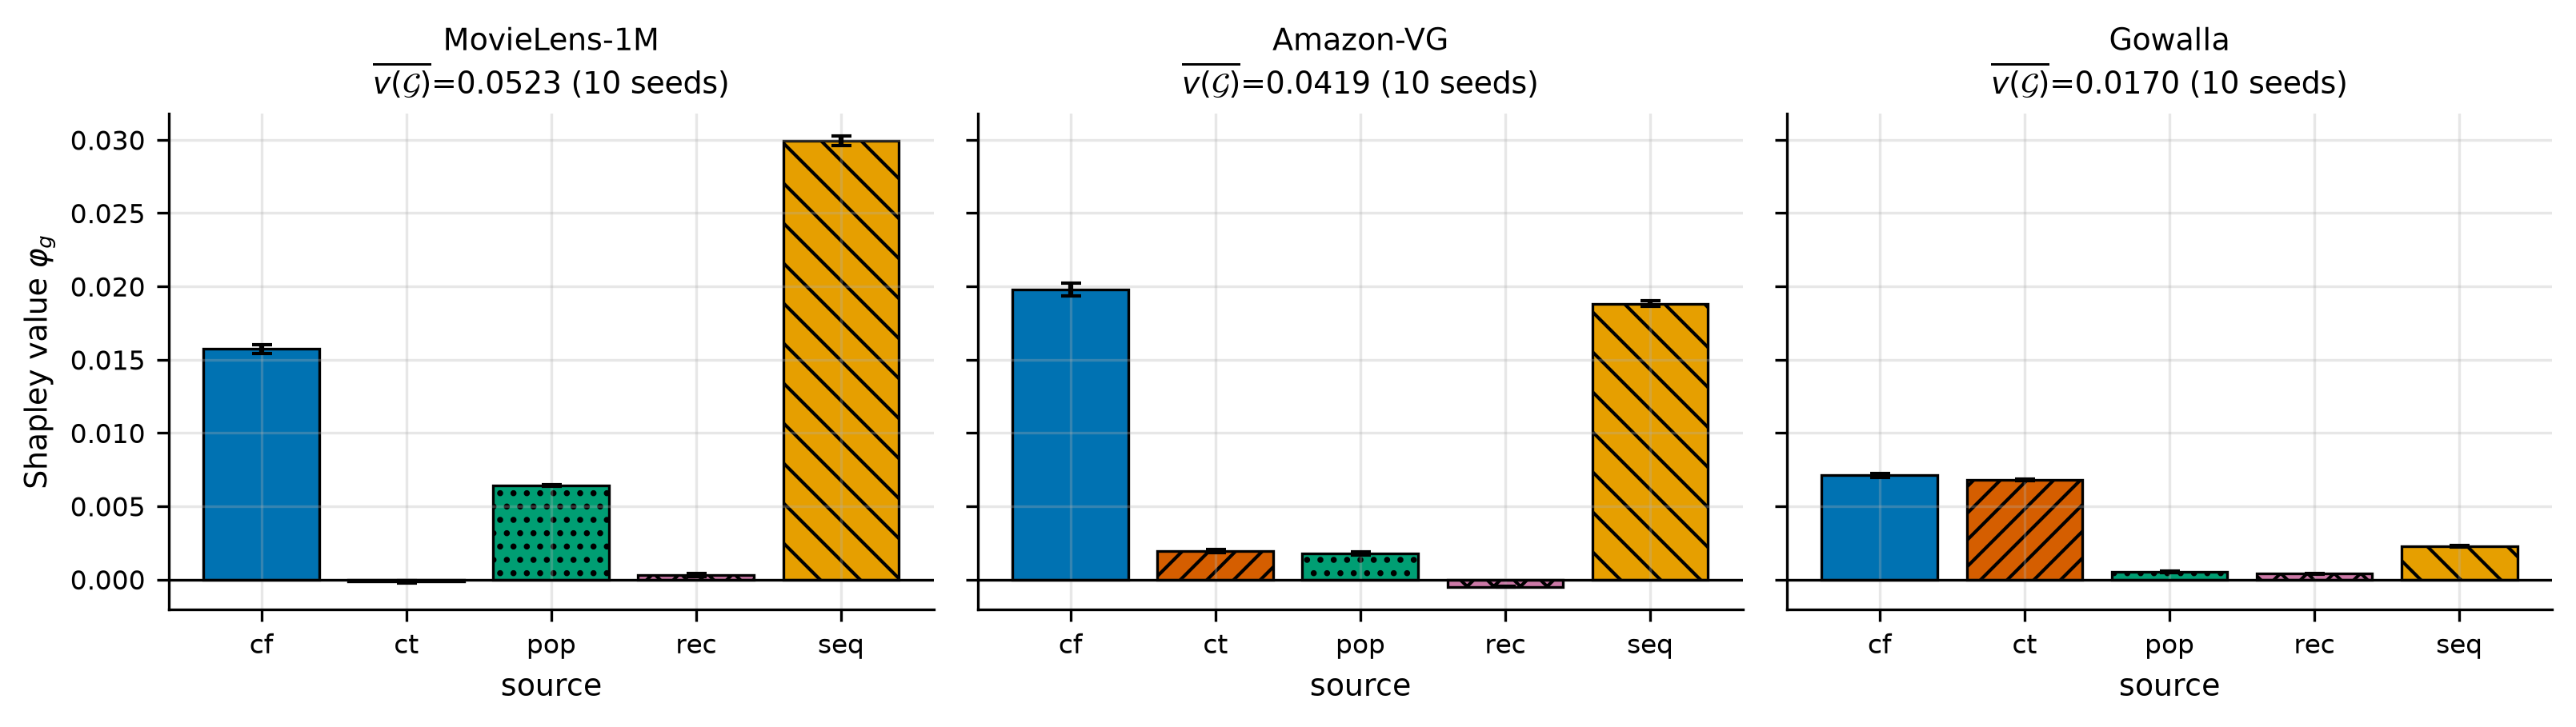
\includegraphics[width=\textwidth]{Fig2.png}
\caption{Per-source Shapley values over seeds 42--51; whiskers show
$\bar{x}\pm t_9\mathrm{SE}$.}
\label{fig:shares}
\end{figure*}

\paragraph{Configuration}\label{sec:hyperparams}

Table~\ref{tab:hyper} lists every value that affects a reported number. All are
fixed in a version-controlled configuration file before the runs and are not
tuned per corpus or per coalition; where a value was amended after the first
runs, the file records the date and the reason. We report them in the paper
rather than only in the repository, because a frozen configuration is not a
substitute for a stated one.

\begin{table*}[tp]
\caption{Experimental configuration.}
\label{tab:hyper}
\footnotesize
\setlength{\tabcolsep}{3pt}
\begin{tabularx}{\textwidth}{@{}ll>{\raggedright\arraybackslash}p{0.26\textwidth}X@{}}
\toprule
Component & Parameter & Value & Note \\
\midrule
$cf$  & latent factors        & $64$    & ALS, implicit feedback \\
      & confidence scaling    & $\alpha = 1$, $c_{ui} = 1 + \alpha r_{ui}$ & binarised $r_{ui}$ \\
      & regularisation        & $0.1$   & \\
      & alternating iterations& $15$    & \\
$ct$  & TF--IDF vocabulary    & $5000$  & token pattern \texttt{\textbackslash S+} \\
$pop$ & decay half-life       & $180$ d & exponential \\
$rec$ & content clusters      & $20$    & argmax over a $20$-component truncated
                                            SVD of a separate $2\,000$-vocabulary
                                            TF--IDF item matrix (no $k$-means);
                                            \texttt{random\_state} $=$ seed \\
      & TF--IDF vocabulary      & $2000$  & separate from $ct$'s $5000$ \\
      & decay half-life       & $30$ d  & \\
$seq$ & embedding dimension   & $64$    & PPMI--SVD \\
      & PPMI shift            & $k_{\mathrm{s}} = 1$, so $\log k_{\mathrm{s}} = 0$ & unshifted: the configuration is plain PPMI--SVD \\
      & co-occurrence window  & $5$     & \\
\midrule
Game  & $N_{\max}$            & $600$ / $600$ / $11\,623$ & ML-1M / Amazon-VG / Gowalla \\
      & ridge $\lambda$       & $1.0^{\dagger}$ & summed-loss parameter. The
        comparable averaged-loss value $\lambda/|\mathcal U_{\rm fit}|$ is
        $1.66\times10^{-4}$, $1.40\times10^{-4}$ and $1.13\times10^{-4}$ for
        ML-1M, Amazon-VG and Gowalla, so $\lambda=1$ is not the same
        effective penalty across corpora \\
      & NDCG cutoff $K$       & $10$    & \\
      & empty-coalition baseline & $\mathbb{E}[\NDCG]$ & Equation~(\ref{eq:baseline}); deterministic, no seed \\
      & ranking tie rule      & score, then item index & exact total order; no tolerance relation \\
      & initial per-source depth & $\lceil N_{\max}/n \rceil$ & $120$ for $N_{\max}=600$, equal for every source \\
      & candidate growth iters& $10$    & $N_g \gets N_g + \lceil (N_{\max} - |C_u|)/n \rceil$ per pass \\
      & recall gate           & $0.60$  & see Section~\ref{sec:preconditions} \\
      & materiality threshold & $10^{-3}$ & reporting only, not a theorem \\
\midrule
Fusion& segments             & $4$     & activity $\times$ recency, median splits \\
      & softmax $\tau$        & $\{0.001, 0.01, 0.1\}^{\dagger}$ & validation-selected \\
      & shrinkage $\gamma_{\mathrm{shrink}}$ & $\{0, 0.5, 1\}^{\dagger}$ & validation-selected \\
\midrule
LightGCN & factors / layers   & $64$ / $3$ & contextual reference only \\
      & epochs / lr / reg     & $40$ / $0.01$ / $10^{-4}$ & \\
SASRec& dim / max length      & $64$ / $50$ & contextual reference only \\
      & blocks / epochs / lr  & $2$ / $25$ / $0.05$ & \\
\midrule
Protocol & seeds              & $42$--$51$ (run-to-run summaries) & seed $42$ alone for labelled single-run diagnostics \\
      & source random state   & seed & passed to ALS and every truncated SVD \\
      & split                 & leave-last-out & test $=$ last, validation $=$ second-last \\
      & tie-break             & (timestamp, record index) & \\
\bottomrule
\end{tabularx}
\smallskip
\noindent\footnotesize $^{\dagger}$Selected on a MovieLens pilot and then
frozen. All other values are prespecified implementation settings and were not
tuned separately by corpus or coalition; $N_{\max}$ alone varies by corpus.
\end{table*}

\begin{table*}[tp]
\caption{Repeat-event audit; masked test items yield zero payoff for every
coalition.}
\label{tab:repeats}
\small
\begin{tabular}{@{}lrrrr@{}}
\toprule
Corpus & Users & Val.\ $=$ test item & Test item in train & Repeat events \\
\midrule
MovieLens-1M & 6\,035 & $0$ ($0.00\%$)    & $0$ ($0.00\%$)      & $0.00\%$ \\
Amazon-VG    & 7\,120 & $430$ ($6.04\%$)  & $198$ ($2.78\%$)    & $5.27\%$ \\
Gowalla      & 8\,865 & $1\,260$ ($14.21\%$) & $4\,424$ ($49.90\%$) & $52.61\%$ \\
\bottomrule
\end{tabular}
\par\smallskip
\begin{minipage}{0.92\textwidth}
\raggedright\footnotesize
$^{\ast}$Final source-symmetric candidate rule; these are the seed-42 main
results used elsewhere in the paper. $^{\dagger}$Legacy candidate rule,
retained as a sensitivity analysis only: these rows predate the truncation-key
regeneration and are not artefact-matched to the refitted-head row. The table
therefore compares \emph{orderings} across estimands, not numerical estimates
from a single artefact.
\end{minipage}
\end{table*}

\paragraph{Preprocessing and subsampling}
MovieLens-1M is binarised at rating $\geq 4$, which is why the as-used
interaction count is $575\,276$ rather than one million. Gowalla and Amazon-VG
are filtered to a $10$-core and binarised (Amazon at rating $\geq 4$; Gowalla
check-ins are implicit). Both are then subsampled by drawing users uniformly at
random without replacement under seed $42$, retaining all interactions of the
drawn users; the number of users is \emph{derived} from a declared memory
budget rather than chosen, since five dense score matrices at
$8\,865 \times 82\,134$ already occupy $14.6$\,GB and the full corpus would
need $129$\,GB. Item vocabularies are re-indexed after subsampling, so the
catalogue sizes in Table~\ref{tab:preconditions} are post-subsampling.


\section{Results and discussion}\label{sec:results_discussion}

\subsection{Implementation checks against known axiomatic constraints}\label{sec:recovery}

On observational data the correct allocation is unknown. This section therefore
does not validate the real-system magnitudes; it checks whether the
implementation satisfies constraints known in advance. Duplicate injection
fixes an exchangeability requirement, while the analytic games check exact
magnitudes for synthetic characteristic functions.

\paragraph{Design}
We inject a near-duplicate of an existing source $g$ at the level of raw
source scores, before any $z$-normalisation:
%
\begin{equation}
s_{g_{\mathrm{dup}}}(u,i) = s_g(u,i) + \eta\,\hat\sigma_g\,\epsilon_{u,i},
\qquad
\epsilon_{u,i} \overset{\mathrm{i.i.d.}}{\sim} \mathcal N(0,1),
\label{eq:dup}
\end{equation}
%
and re-run the game with six players. Here $g$ is $cf$ unless stated
otherwise, $\hat\sigma_g$ is the standard deviation of $s_g$ over all
eligible (user, item) entries, one scalar per source rather than one per user,
and the perturbations $\epsilon_{u,i}$ are drawn independently for each
(user, item) pair from a generator seeded with the run seed. Ineligible
entries stay masked, so the clone inherits exactly the eligibility pattern of
its original. Setting $\eta = 0$ gives an exact duplicate. The candidate set
is built \emph{before} injection and held fixed, so the clone never enters
retrieval and the only thing that changes is the player set.

\paragraph{What is known in advance, and what is not}
At $\eta = 0$ the original and duplicated sources are exchangeable in the
declared game, so any rule satisfying the symmetry axiom must assign them equal
values. This gives a checkable constraint that does not depend on the data.
Property~\ref{prop:loo} suggests a second outcome: leave-one-out should
collapse toward zero for \emph{both} members, since either alone is
dispensable. \textbf{This one is not structurally guaranteed under our fitted
game, and we do not treat it as such.} Duplicating a column in a ridge
regression is not prediction-invariant: two identical columns share the
penalty, so the effective regularisation on their common direction is halved
and the fitted scores can move. Exchangeability of the pair is guaranteed;
redundancy of the coalition \emph{values} is an empirical question. We
therefore write $g'=g_{\mathrm{dup}}$ and measure it by reporting
\begin{equation}
\begin{aligned}
\Delta_{\mathrm{red}}
&= \max_{S \subseteq \G\setminus\{g,g'\}} d(S),\\
d(S)
&= \max\left\{
\begin{aligned}
&|v(S\cup\{g\})-v(S\cup\{g,g'\})|,\\
&|v(S\cup\{g'\})-v(S\cup\{g,g'\})|
\end{aligned}
\right\}
\end{aligned}
\label{eq:reddev}
\end{equation}
alongside the symmetry error, and we run the diagnostic at both the frozen
$\lambda$ and at $\lambda = 0$. The latter matters because ordinary least
squares \emph{is} invariant to a repeated column, since with the minimum-norm solution a shared coefficient splits evenly and predictions are unchanged, so $\lambda = 0$ turns the redundancy prediction into a structural guarantee and
isolates whether any deviation at the frozen $\lambda$ is due to
regularisation.

We are deliberately precise about the limits of this design.
\textbf{Duplication does not conserve credit}, and it would be wrong to require
that it should. The combined Shapley value of a cloned pair need not equal the
original player's pre-duplication value: in the two-player monotone game
$v(g)=7$, $v(h)=8$, $v(g,h)=8$ one has $\varphi_g = 3.5$, whereas replacing
$g$ by perfect substitutes $g_1,g_2$ gives
$\varphi_{g_1} = \varphi_{g_2} = 7/3$ and a pair sum of $14/3 \approx 4.67$.
Clone insertion redistributes credit among \emph{all} players, a sensitivity of
Shapley allocations to replication that is known in the cooperative-game
literature~\citep{han2022replication}. Our own runs show the same effect: on
MovieLens-1M the pair sum is $0.02156$ against a pre-injection
$\varphi_{cf} = 0.01520$ in the same injection run, a ratio of $1.42$. We therefore treat the pair sum as
a \emph{diagnostic}, not a requirement, and the experiment as a symmetry and
implementation check rather than as recovery of absolute credit.

\begin{table*}[tp]
\caption{MovieLens-1M duplicate-source diagnostics ($cf$ clone, $\eta=0$).}
\label{tab:recovery}
\begin{tabular}{@{}lrrrrr@{}}
\toprule
Corpus & $\lambda$ & Sym.\ err. & $\Delta_{\mathrm{red}}$ &
$\varphi(cf) = \varphi(cf_{\mathrm{dup}})$ &
$\LOO(cf)$, $\LOO(cf_{\mathrm{dup}})$ \\
\midrule
\multirow{2}{*}{MovieLens-1M} & frozen & $0.0$ & $0.0$ & $0.010781$ & $0.000000$, $0.000000$ \\
                              & $0$    & $0.0$ & $0.0$ & $0.010781$ & $0.000000$, $0.000000$ \\
\bottomrule
\end{tabular}
\end{table*}

Table~\ref{tab:recovery} reports the outcome. The result is unambiguous and
reproducible: Shapley satisfies symmetry exactly
in every condition. LOO returns \textbf{exactly zero} for both members of every pair, not approximately but exactly, because $v(\G) = v(\G \setminus \{g\})$ holds numerically when a perfect substitute
remains in the coalition. Shapley splits the shared capability evenly, giving
each clone $0.01078$ against $0.01520$ for $cf$ before injection, a pair sum of
$0.02156$: the split is exact, and the pair is worth more together than the
single source was, which is the non-conservation discussed above.

The practical reading needs care. It would overstate the result to say an
engineer would retire both duplicates and lose the capability. A
sequential procedure would re-evaluate the system after the first removal and
would not make that error. The narrower point, which is the one the diagnostic
establishes, is that grand-coalition LOO does not \emph{distribute} shared
credit: it can report zero for each of two perfect substitutes while the
capability they share is valuable, so it cannot be used as a simultaneous
allocation rule. Shapley symmetry assigns exchangeable players equal credit and
does not have this failure. Here that difference is measured rather than
argued.

\paragraph{Graceful degradation}
As $\eta$ grows the duplicate becomes a noisier copy and exact redundancy
weakens. LOO becomes non-zero but erratic in sign, which is the behaviour
Lemma~\ref{lem:eps}(i) describes for $\varepsilon$-redundancy.

\subsection{Verifying the aggregation}\label{sec:validating}

\paragraph{Analytic games with known Shapley vectors}\label{sec:analytic}

Duplicate injection tests symmetry, but symmetry alone does not validate
\emph{magnitudes}: a method that halved every value would still pass it. We
therefore also evaluate six analytic games whose Shapley vector is known in
closed form, chosen to span the structures our real games might exhibit
(Table~\ref{tab:analytic}). These are unit tests of the aggregation, not
evidence about recommender data; they establish that the enumeration in
Equation~(\ref{eq:shapley}) is implemented correctly, which is a precondition for interpreting
anything computed with it.

\begin{table*}[tp]
\caption{Exact Shapley recovery on six analytic games.}
\label{tab:analytic}
%% \small and a p{} column: the characteristic functions are long enough
%% that `l' pushed this table past the text block.
\small
\begin{tabular}{@{}lp{0.44\textwidth}cc@{}}
\toprule
Game & Characteristic function $v(S)$ & Expected $\varphi$ & Max error \\
\midrule
Additive     & $\sum_{g\in S} c_g$, \ $c=(3,2,1)$                & $(3, 2, 1)$  & $0$ \\
Substitutes  & $4\cdot\mathbb{1}[\{s_1,s_2\}\cap S \neq \varnothing] + \mathbb{1}[x\in S]$
                                                                  & $(2, 2, 1)$  & $0$ \\
Complements  & $6\cdot\mathbb{1}[\{c_1,c_2\}\subseteq S] + 2\cdot\mathbb{1}[x\in S]$
                                                                  & $(3, 3, 2)$  & $0$ \\
Null player  & $\sum_{g\in S\cap\{a,b\}} c_g$, \ $c=(3,2)$        & $(3, 2, 0)$  & $0$ \\
Harmful      & $5\cdot\mathbb{1}[a\in S] - 2\cdot\mathbb{1}[\mathit{bad}\in S]$
                                                                  & $(5, -2)$    & $0$ \\
Unanimity    & $9\cdot\mathbb{1}[S = \G]$                          & $(3, 3, 3)$  & $0$ \\
\bottomrule
\end{tabular}
\end{table*}

We additionally verify \emph{additivity}, the remaining uniqueness axiom that
no other diagnostic here exercises: efficiency is a sum constraint, symmetry is
covered by duplicate injection, and the null player has its own game. Summing an additive and a unanimity game, structurally different so the check is not vacuous, gives $\varphi(v_1 + v_2) = \varphi(v_1) + \varphi(v_2)$ to
$4.4\times10^{-16}$.

The null-player and harmful games matter most for this paper. Our fitted games
are non-monotone and produce negative $\varphi_g$ (Section~\ref{sec:results}),
so it is necessary to establish that a negative value is a faithful computation
rather than an artefact of the implementation; the harmful game confirms that
$-2$ is recovered exactly. The null-player game confirms that a source
contributing nothing receives exactly zero, which is the property the
structural audit of Section~\ref{sec:setup} relies on.

\paragraph{Alternative values and pairwise interactions}\label{sec:alternatives}

\paragraph{Other semivalues}
The Shapley value is one member of a family, and a comparator is only
informative if it is genuinely a different member. The size-uniform weighting
$p_k = 1/n$ is not: substituting it into Equation~(\ref{eq:semivalue}) returns
Equation~(\ref{eq:shapley}) exactly, because
$|S|!(n-|S|-1)!/n! = 1/\bigl(n\binom{n-1}{|S|}\bigr)$. It is Shapley written by
coalition size, it satisfies efficiency, and comparing it against Shapley is
vacuous. We note this because the identity is easy to miss.

The distinct comparators we report are Banzhaf, $p_k =
\binom{n-1}{k}2^{-(n-1)}$, and the binomial semivalues $p_k =
\binom{n-1}{k}q^k(1-q)^{n-1-k}$ at $q = 0.25$ and $q = 0.75$, in which each
other source joins the predecessor coalition independently with probability
$q$. Small $q$ favours sources that are valuable in isolation; large $q$
favours sources that still add value once the others are present, so the pair
brackets the redundancy question the paper is about. On MovieLens (seed 42) all
four values induce the \emph{same} source ordering, with $seq$ first
(Kendall $\tau = 1.00$ against Shapley in each case), while their totals differ
widely, $0.05190$ for Shapley against $0.05167$, $0.06992$ and $0.03378$ for
Banzhaf, $q=0.25$ and $q=0.75$. These four totals are a within-platform set
computed on x86-64, so the Shapley entry is the $0.05190$ of
Section~\ref{sec:game} rather than the $0.05136$ seed-42 main-game value
underlying the refitted-head row of Table~\ref{tab:estimands}; only
their ratios are meaningful, and the point of the comparison is that the
\emph{ordering} is identical while the totals are not. Only Shapley sums to $v(\G)$; for the others
only the induced ordering is comparable.

That robustness does \emph{not} extend to the second corpus, and we report the
disagreement rather than confine the comparison to the corpus that supports it.
On Amazon-VG the Banzhaf ordering agrees with Shapley only at
$\tau = 0.60$, and the two disagree on the leading source: Shapley puts $cf$
first, Banzhaf puts $seq$ first. Banzhaf weights every coalition equally,
whereas Shapley up-weights the extreme sizes, so the two diverge exactly where
a source's value depends on how many other sources are present. Amazon-VG is
also the corpus with the strongest substitutive $cf$--$seq$ interaction and no
material sign flip, which is consistent with that reading. The defensible claim
is therefore narrower than a single-corpus result would suggest.

Gowalla sits between the two, and its behaviour is the most informative of the
three. Banzhaf and both binomial semivalues agree with Shapley at
$\tau = 0.80$, and three of the four values put $cf$ first. The exception is
the $q=0.25$ semivalue, which up-weights small coalitions and promotes $ct$
above $cf$. That is not a contradiction of the main result but a second,
independent route to a caveat the paper already states: Shapley separates $cf$
from $ct$ on this corpus by only $0.00037$, and reweighting the coalition
sizes is enough to invert a margin that small. Section~\ref{sec:results}
reaches the same conclusion from user resampling. Under Banzhaf and $q=0.75$
the single transposition instead falls between $pop$ and $rec$, which Shapley
separates by $0.00017$. In every case the value that moves is one of a pair the
main analysis already declines to order.

The three corpora therefore give three different answers, and the honest
summary is the conjunction rather than the best case: the induced ordering is
robust to the choice of semivalue on MovieLens-1M, robust on Gowalla except
for a leading pair the paper already treats as a near-tie, and \emph{not}
robust on Amazon-VG, where the leading source itself changes. A reported
ordering should therefore state which value produced it, and a margin at the
$10^{-4}$ scale should not be read as an ordering at all. Only Shapley sums to
$v(\G)$; the totals differ widely across values
($0.01690$, $0.01438$, $0.02147$ and $0.01102$ on Gowalla), which is why we
compare orderings and not magnitudes.

\paragraph{Pairwise interactions}
Main-effect values cannot by themselves distinguish a source of low value from
a source whose value is absorbed by a redundant partner. We therefore compute a
pairwise interaction index: the classical \emph{Shapley interaction index} of
Grabisch and Roubens~\citep{grabisch1999interaction}. This index differs from
the order-2 Shapley--Taylor
index~\citep{sundararajan2020shapleytaylor}: the two are not interchangeable,
since at $n=5$ their coalition weights differ by up to a factor of $2.5$. We
use Grabisch--Roubens throughout, and note that
Grabisch--Roubens does not satisfy Shapley--Taylor's interaction-efficiency
axiom: the pairwise terms do not sum with the singletons to $v(\G)$. That is
acceptable here because we use them only to \emph{rank} redundancy, which is
all the argument requires. Each pair $\{a,b\}$ receives
%
\begin{equation}
\begin{aligned}
\mathcal{I}_{ab}
  &= \sum_{S \subseteq \G \setminus \{a,b\}}
     \frac{|S|!\,(n - |S| - 2)!}{(n-1)!} \\
  &\quad{}\times \bigl[v(S \cup \{a,b\}) - v(S \cup \{a\}) \\
  &\hspace{5.7em}{}- v(S \cup \{b\}) + v(S)\bigr],
\end{aligned}
\label{eq:interaction}
\end{equation}
%
the averaged second-order discrete derivative. A negative $\mathcal{I}_{ab}$
means the pair jointly contributes less than the sum of their separate
contributions. We read that as negative, or substitutive, interaction
\emph{under the declared game}, which is a game-theoretic statement and not a
demonstration of causal redundancy; a positive value indicates complementarity
in the same sense.

\begin{table}[tbp]
\caption{MovieLens-1M pairwise Shapley interactions over ten stochastic fits.}
\label{tab:taylor}
\centering
\footnotesize
\setlength{\tabcolsep}{2.5pt}
\begin{tabular}{@{}lrcc@{}}
\toprule
Pair & $\mathcal{I}_{ab}$ (10-seed mean) & run interval & Neg.\ seeds \\
\midrule
$cf$--$seq$  & $-0.0542$ & $[-0.0554, -0.0529]$ & $10/10$ \\
$cf$--$pop$  & $-0.0254$ & $[-0.0256, -0.0252]$ & $10/10$ \\
$ct$--$pop$  & $-0.0027$ & $[-0.0029, -0.0025]$ & $10/10$ \\
$pop$--$rec$ & $-0.0017$ & $[-0.0019, -0.0016]$ & $10/10$ \\
$cf$--$rec$  & $-0.0011$ & $[-0.0014, -0.0009]$ & $10/10$ \\
$rec$--$seq$ & $-0.0011$ & $[-0.0014, -0.0009]$ & $10/10$ \\
$ct$--$rec$  & $+0.0004$ & $[+0.0003, +0.0006]$ & $0/10$ \\
$ct$--$seq$  & $+0.0012$ & $[+0.0009, +0.0014]$ & $0/10$ \\
$cf$--$ct$   & $+0.0020$ & $[+0.0016, +0.0023]$ & $0/10$ \\
$pop$--$seq$ & $+0.0059$ & $[+0.0056, +0.0061]$ & $0/10$ \\
\bottomrule
\end{tabular}
\end{table}

Table~\ref{tab:taylor} localises the negative interactions associated with the MovieLens sign flip.
The two most negative pairs are $cf$--$seq$ ($-0.054$) and $cf$--$pop$ ($-0.025$),
both stable in sign on all ten seeds:
collaborative filtering has the strongest substitutive interaction with the sequential and popularity
sources, which is why removing it from the grand coalition costs so little and
why leave-one-out scores it below zero. Only one of these, $cf$--$pop$, was
declared in advance (Section~\ref{sec:setup}); $cf$--$seq$ was not, and the other
declared overlap $rec$--$ct$ comes out slightly \emph{positive} at $+0.0004$. We
therefore claim partial rather than complete recovery of the pre-declared
structure. Every
pair in Table~\ref{tab:taylor} keeps its sign on all ten seeds, so the
interaction ordering does not rest on a single run.

\paragraph{The redundancy mechanism replicates on Gowalla}
The interaction index is cheap once the $32$ coalition values exist, so we
computed it on the other two corpora as well; those are seed-42 values under
the legacy candidate rule and we label them as such. The test is whether the
source carrying each material sign disagreement is also the one with the
strongest substitutive interaction. It is. On Gowalla the most negative pair is
$ct$--$pop$ at $-0.0083$, and $pop$ is the source whose ranking-stage
leave-one-out turns negative, exactly as $cf$ is on MovieLens-1M, where the two
most negative pairs both involve $cf$. On Amazon-VG, which has no material
disagreement, the most negative pair is $cf$--$seq$ at $-0.0445$ while $cf$
carries the largest positive gap rather than a sign flip, so a strong
substitutive interaction is not by itself sufficient to produce one. The
mechanism is therefore consistent across the two corpora that exhibit the
phenomenon, and the negative case shows the interaction index alone does not
predict it.

\subsection{Attribution on real systems}\label{sec:results}

\begin{table*}[tp]
\caption{Ten-seed ranking-stage LOO and Shapley attribution. Brackets are
run-to-run intervals $\bar x \pm t_{0.975,9}\,s_x/\sqrt{10}$. The quantity
this paper contrasts is the paired gap $\Delta_g = \varphi_g - \LOOr(g)$, so it
carries its own interval, computed per seed and then aggregated rather than
differenced from the two marginal means; this is why the gap interval is not
the difference of the two columns beside it. ``Gap sign'' counts the fits on
which $\Delta_g$ keeps the sign of its mean. Fourteen of the fifteen cells are
unanimous; the exception is $rec$ on MovieLens-1M at $9/10$, whose gap is
$0.4\%$ of $v(\G)$ and which the paper does not interpret. Both material
disagreements have gap intervals excluding zero, at $38.8\%$ ($cf$,
MovieLens-1M) and $12.2\%$ ($pop$, Gowalla) of the respective $v(\G)$.}
\label{tab:loo}
\small
\setlength{\tabcolsep}{2.5pt}
\begin{tabular*}{\textwidth}{@{\extracolsep{\fill}}llrcrc@{}}
\toprule
Corpus & Source & $\LOOr$ & Shapley [run interval]
       & Gap $\varphi_g-\LOOr$ [run interval] & Gap sign \\
\midrule
MovieLens-1M & $cf^{\dagger}$ & $-0.00457$ & $+0.01573\ [+0.01542,+0.01604]$ & $+0.02030\ [+0.02007,+0.02053]$ & $10/10$ \\
             & $ct^{\ddagger}$ & $+0.00052$ & $-0.00016\ [-0.00024,-0.00008]$ & $-0.00068\ [-0.00088,-0.00047]$ & $0/10$ \\
             & $pop$ & $+0.00070$ & $+0.00643\ [+0.00638,+0.00649]$ & $+0.00573\ [+0.00551,+0.00596]$ & $10/10$ \\
             & $rec$ & $+0.00010$ & $+0.00032\ [+0.00022,+0.00042]$ & $+0.00022\ [+0.00003,+0.00040]$ & $9/10$ \\
             & $seq$ & $+0.01745$ & $+0.02993\ [+0.02963,+0.03024]$ & $+0.01249\ [+0.01209,+0.01288]$ & $10/10$ \\
\midrule
Amazon-VG    & $cf$ & $+0.00890$ & $+0.01980\ [+0.01937,+0.02022]$ & $+0.01089\ [+0.01062,+0.01117]$ & $10/10$ \\
             & $ct$ & $+0.00011$ & $+0.00195\ [+0.00183,+0.00207]$ & $+0.00183\ [+0.00165,+0.00201]$ & $10/10$ \\
             & $pop$ & $+0.00394$ & $+0.00178\ [+0.00166,+0.00190]$ & $-0.00216\ [-0.00244,-0.00188]$ & $0/10$ \\
             & $rec^{\ddagger}$ & $+0.00014$ & $-0.00049\ [-0.00053,-0.00046]$ & $-0.00063\ [-0.00069,-0.00057]$ & $0/10$ \\
             & $seq$ & $+0.00761$ & $+0.01883\ [+0.01865,+0.01900]$ & $+0.01122\ [+0.01107,+0.01138]$ & $10/10$ \\
\midrule
Gowalla      & $cf$ & $+0.00743$ & $+0.00711\ [+0.00698,+0.00725]$ & $-0.00032\ [-0.00039,-0.00025]$ & $0/10$ \\
             & $ct$ & $+0.00547$ & $+0.00678\ [+0.00672,+0.00683]$ & $+0.00131\ [+0.00121,+0.00141]$ & $10/10$ \\
             & $pop^{\dagger}$ & $-0.00156$ & $+0.00051\ [+0.00046,+0.00056]$ & $+0.00207\ [+0.00197,+0.00217]$ & $10/10$ \\
             & $rec$ & $+0.00001$ & $+0.00040\ [+0.00038,+0.00042]$ & $+0.00039\ [+0.00037,+0.00041]$ & $10/10$ \\
             & $seq$ & $+0.00093$ & $+0.00225\ [+0.00219,+0.00230]$ & $+0.00132\ [+0.00125,+0.00138]$ & $10/10$ \\
\bottomrule
\end{tabular*}
\par\smallskip
{\raggedright\footnotesize $^{\dagger}$Material sign flip;
$^{\ddagger}$sign flip below the $10^{-3}$ materiality threshold.\par}
\end{table*}

\begin{figure*}[tp]
\centering
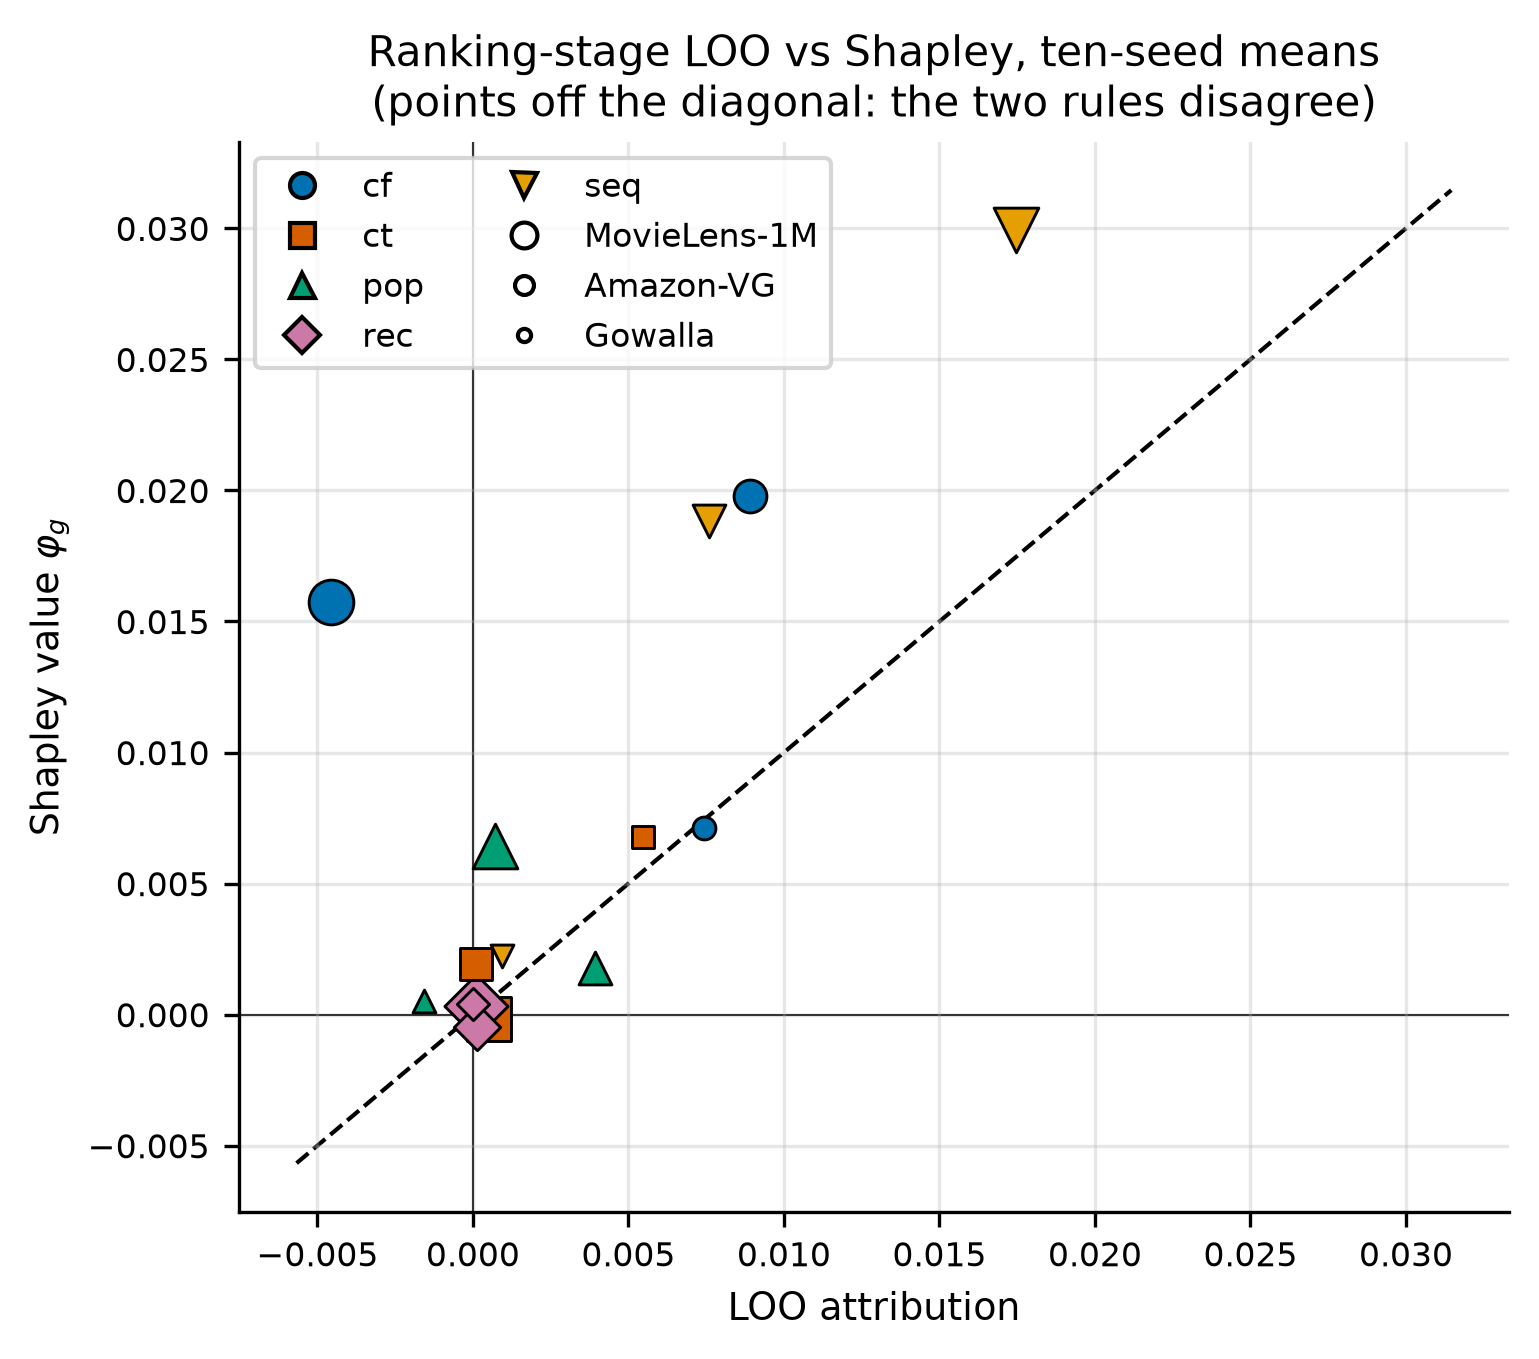
\includegraphics[width=0.7\textwidth]{Fig3.png}
\caption{Ten-seed mean Shapley versus ranking-stage LOO; the diagonal denotes
equality.}
\label{fig:scatter}
\end{figure*}

Table~\ref{tab:loo} gives the per-source comparison and
Figure~\ref{fig:scatter} plots it. Material sign disagreement occurs on
MovieLens and Gowalla, while Amazon-VG provides a negative case.

\paragraph{What is consistent, and what is not}
Two of the three corpora contain a \emph{material} sign disagreement, one where the gap exceeds $10^{-3}$, the same threshold we apply to monotonicity.
On MovieLens it is $cf$: Shapley scores it $+0.01573$, the second most valuable
source in the system, where $\LOOr$ scores it $-0.00457$, meaning its removal
\emph{improves} the fixed-candidate ranking game. The gap is $0.02030$ $[+0.02007, +0.02053]$, or $38.8\%$ of the
ten-seed $v(\G) = 0.05225$, and it is positive on $10/10$ seeds. On Gowalla it
is $pop$, at $12.2\%$ of $v(\G) = 0.01705$ (gap $0.00207$; the ratio is
$0.1216$) and likewise $10/10$: $\LOOr$ scores
the popularity signal negative where Shapley scores it positive. All figures in
this paragraph are ten-seed means, so the gap and the grand value are at the
same aggregation level; the brackets describe run-to-run variation over
stochastic fits on the fixed datasets.

Amazon-VG has no material disagreement. Its only sign flip, on $rec$, is
$0.00063$, a practically negligible magnitude even though the Shapley
run-to-run interval excludes zero. We state this plainly because it bounds the claim: it would be wrong to say
that \emph{every} system contains a sign disagreement. The accurate statement
is weaker: material sign disagreement between the
two rules occurs on two of the three systems studied here and is absent on the
third. Three corpora cannot estimate how common it is in the wider population
of hybrid recommenders; what they establish is that it is possible and can be
large. Nothing in
either rule announces in advance whether a given system will exhibit it.

\paragraph{Within-run regularisation sensitivity}
At seed $42$, we swept the summed-loss parameter $\lambda$ over eight orders of magnitude,
$10^{-5}$ to $10^{3}$, recomputing the full game at each value. The material
flips are invariant: $cf$ flips on MovieLens and $pop$ flips on Gowalla at
\emph{every} $\lambda$ tested, and they are the only material flips on those
corpora throughout. Amazon-VG has none until $\lambda = 10^{3}$, where the
head is so heavily penalised that $ct$ acquires one; we regard that endpoint as
degenerate rather than informative. This establishes within-run sensitivity to
the chosen penalty, not cross-seed or cross-corpus invariance. Figure~\ref{fig:robustness}
shows the representative points $0.1$, $1$, and $10$; the conclusions above
refer to the complete evaluated grid. Because Eq.~\eqref{eq:head}
uses a summed loss, the numerical values are not portable across corpus sizes.

\begin{figure*}[tp]
\centering
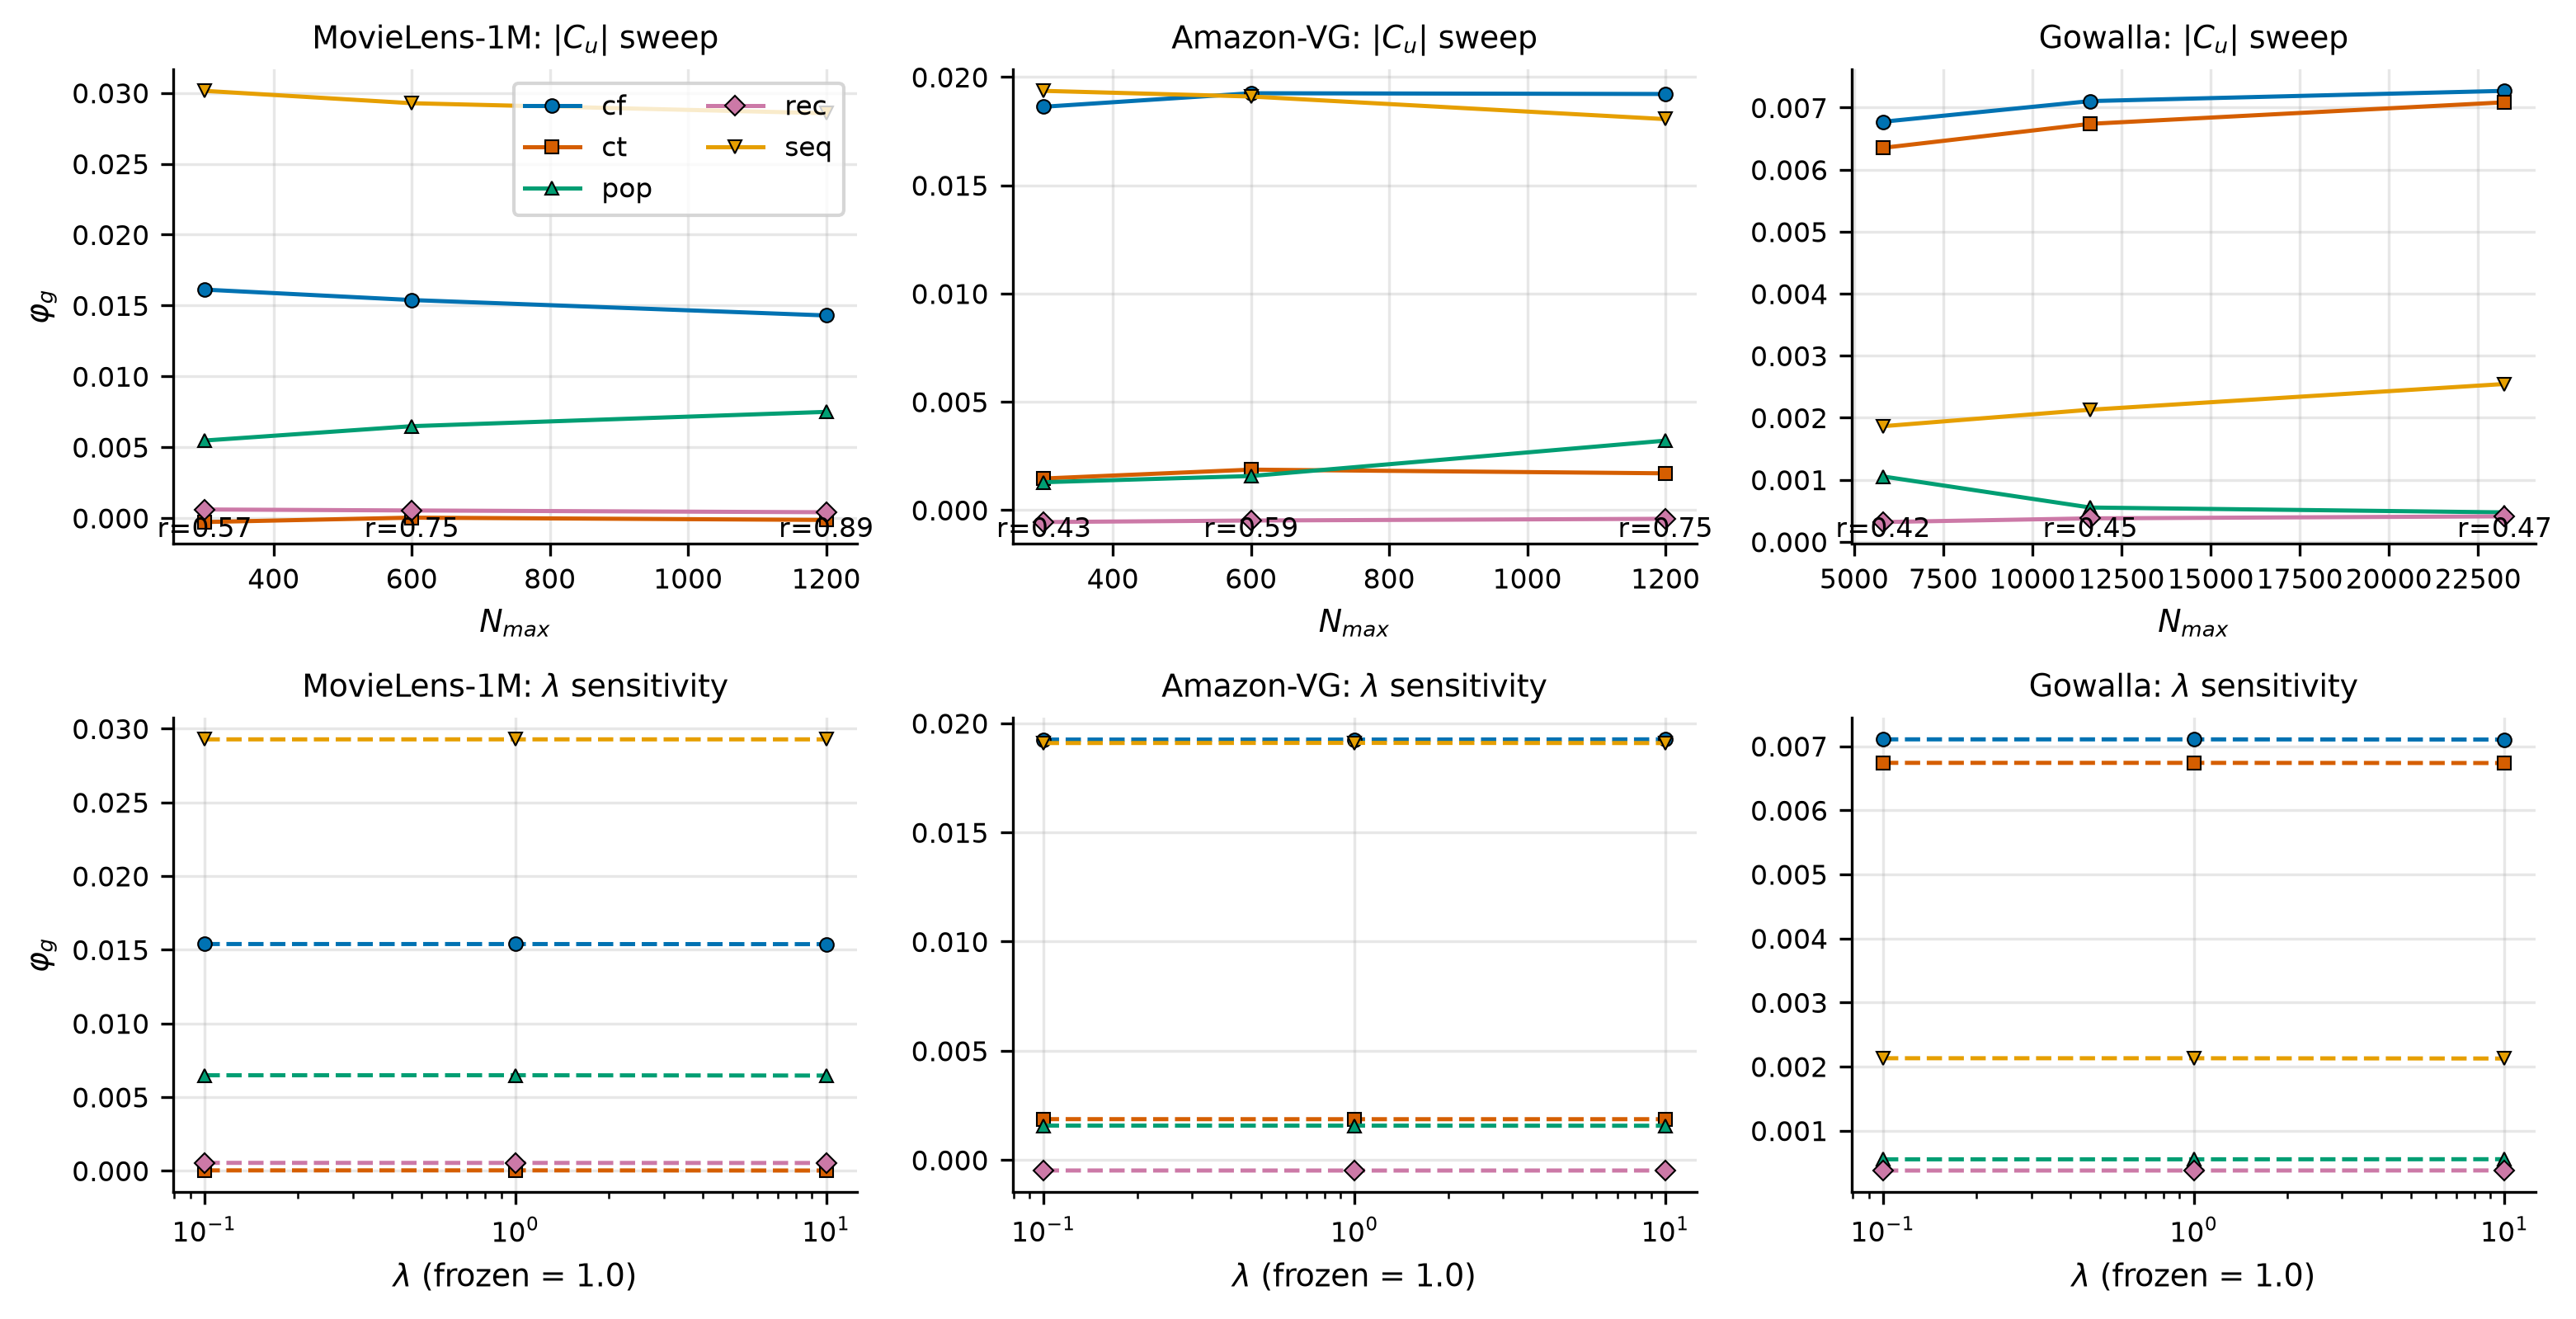
\includegraphics[width=\textwidth]{Fig7.png}
\caption{Candidate-cap and ridge-penalty sensitivity at seed 42; labels show
candidate recall.}
\label{fig:robustness}
\end{figure*}

Two robustness checks are available for the Gowalla result. The corpus was run
at three subsample sizes, $4\,652$, $5\,910$ and $8\,865$ users, drawn to
different memory budgets. The material $pop$ disagreement is present at all
three, and $pop$ is the only material flip in each case: at the two larger
sizes it is $9.9\%$ and $12.2\%$ of $v(\G)$. A $1.9\times$ change in corpus
size therefore does not create or destroy it. We report the largest run
throughout.

The magnitudes are \emph{not} stable, however, and neither is the top source.
We report this against our own convenience. A full ten-seed repetition at a
smaller memory budget draws $4\,652$ of $8\,865$ users and $59\,597$ of
$82\,134$ items, which also raises the frozen $N_{\max} = 11\,623$ from
$14.2\%$ to $19.5\%$ of the catalogue. Under that resampling every Gowalla sign
is preserved and the material $pop$ flip survives, but individual values move
by more than a factor of two, Kendall $\tau$ against the full run falls to
$0.80$, and the top-ranked source exchanges between $cf$ and $ct$, the two
sources the full run separates by only $0.00033$. We therefore do not claim a
stable top source on Gowalla, and the $cf \succ ct$ ordering reported above
should be read as a near-tie rather than a finding. The same repetition on
MovieLens-1M and Amazon-VG, whose user caps are not budget-bound and whose
corpora are therefore identical across the two runs, preserves the ordering
exactly ($\tau = 1.00$, same top source). The conclusion is narrow: on the
sparsest corpus, which is also the one that fails the recall gate by the widest
margin, only the signs and the material disagreement survive resampling.

The corollary is that a single-corpus reading would have been actively
misleading. On MovieLens alone one would conclude that collaborative filtering
is the source ablation systematically undervalues. Gowalla's material flip
falls on $pop$ instead, and Amazon-VG has none. The results are consistent
with the
\emph{mechanism} that disagreement tracks redundancy, though the interaction
analysis supports that reading directly only on MovieLens. What certainly does
not generalise is the identity of the affected source, or the guarantee that
one exists at all.

\paragraph{Mechanism}
The account is \emph{qualitatively} the one Property~\ref{prop:loo} describes,
though the property does not formally apply: all three fitted games are
non-monotone (Table~\ref{tab:preconditions}), so the positivity conclusion is
unavailable and what follows is interpretation rather than theorem. A source
whose signal is covered by others costs little when removed from the
\emph{grand} coalition, because the others absorb its role, and ablation
observes only that single contrast. SignalShap averages the source's
contribution over all $16$ coalitions in which it can appear, including those
where nothing covers for it, and so recovers value that the overlap conceals.
On MovieLens the collaborative signal overlaps with the sequential and
popularity signals; on Gowalla it is the popularity signal that is covered, by
a geographic content signal that is essentially tied with $cf$ at the top of
the ranking ($0.00678$ against $0.00711$, an ordering that resampling
reverses).

\paragraph{Ranking stability}
The per-corpus orderings are
$seq \succ cf \succ pop \succ rec \succ ct$ (MovieLens),
$cf \succ seq \succ ct \succ pop \succ rec$ (Amazon-VG), and
$cf \succ ct \succ seq \succ pop \succ rec$ (Gowalla, where the leading pair is
within $0.00033$ and exchanges under resampling). Pairwise Kendall $\tau$
between corpora is $0.40$ (MovieLens--Amazon), $0.20$ (MovieLens--Gowalla) and
$0.80$ (Amazon--Gowalla), none significant at $n=5$ sources. We therefore make
no cross-corpus consistency claim; identical near-zero values from sources with
no usable input would inflate this comparison and are not treated as evidence
of agreement.

Score-vector association has a descriptive correlation of $r=0.525$ with the
attribution shift on MovieLens across the ten source pairs. This is not a test
of Lemma~\ref{lem:eps}: the lemma defines substitutability through coalition
values, whereas the auxiliary statistic compares per-user score rankings. The
ten pair observations also share sources and are not independent. We therefore
report the coefficient only as an exploratory description, without a
redundancy or significance claim.

Figure~\ref{fig:redundancy} shows the pairwise structure directly.

\begin{figure*}[tp]
\centering
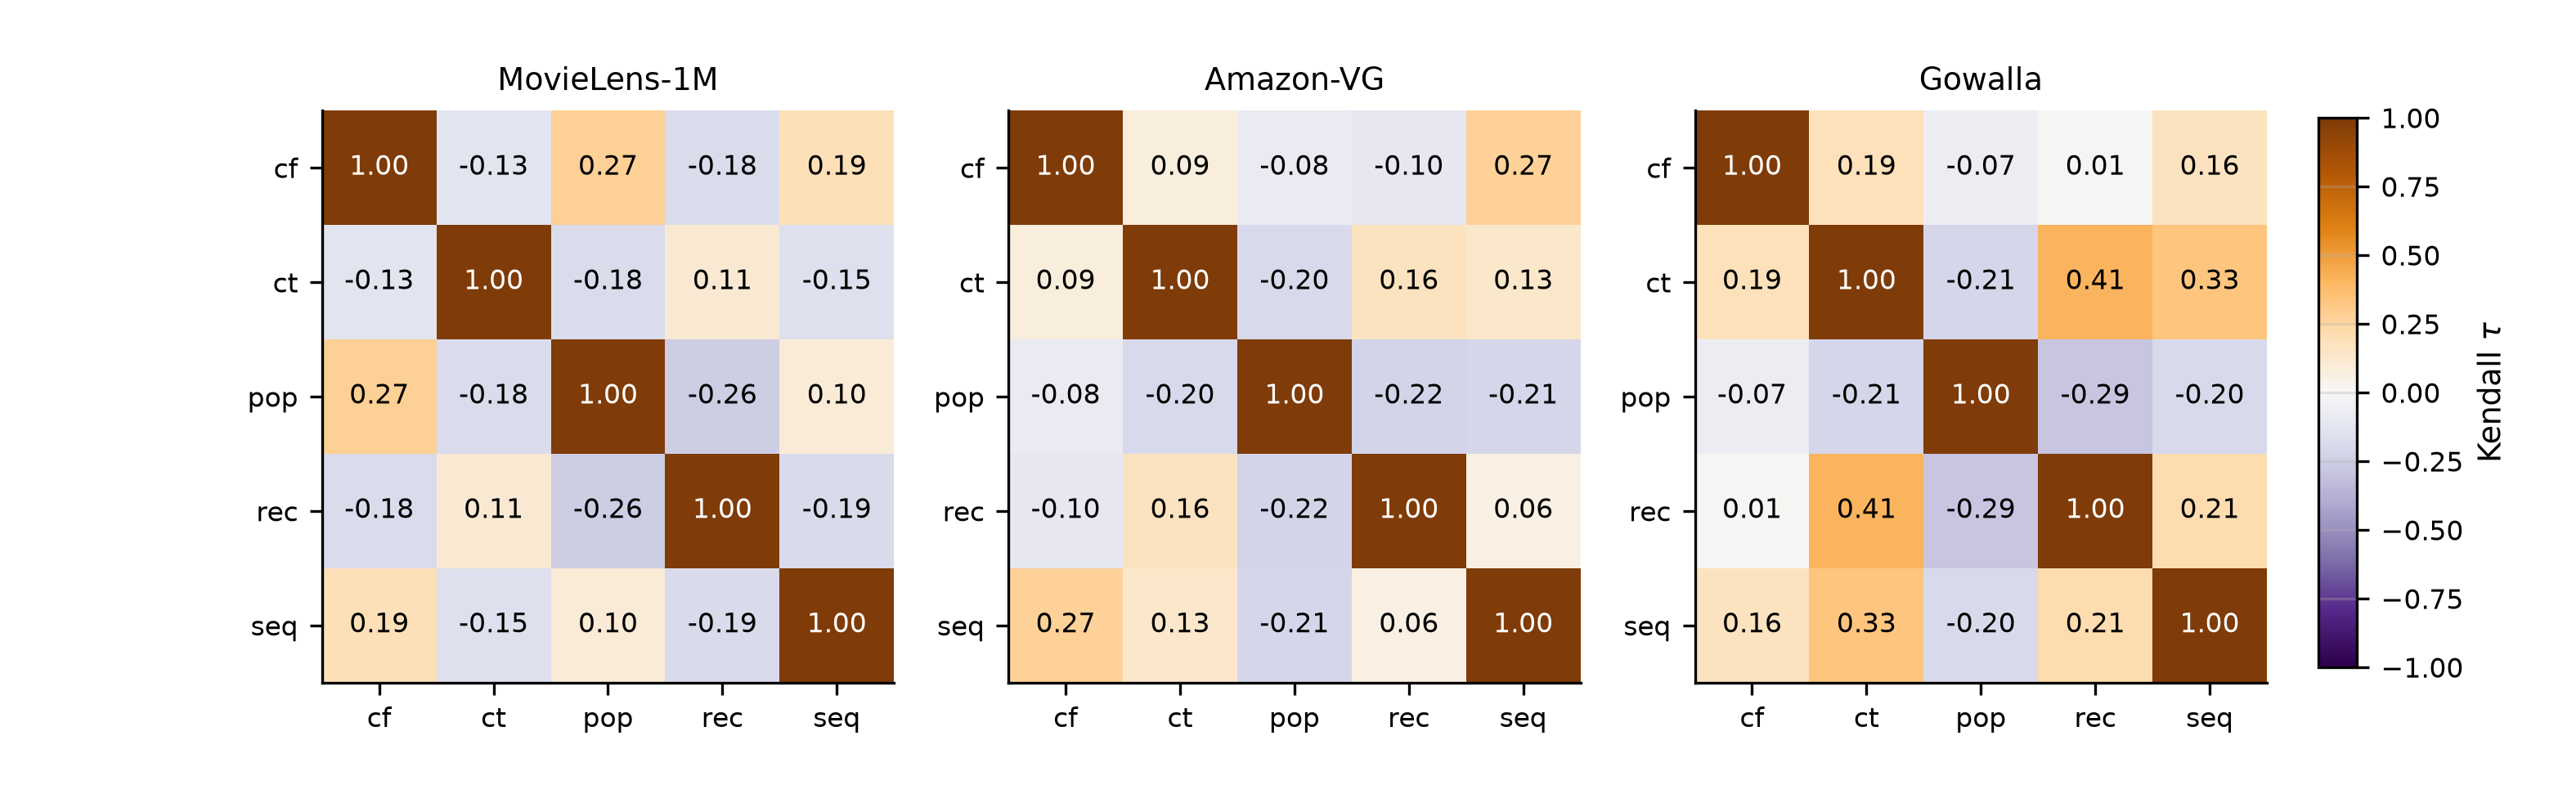
\includegraphics[width=\textwidth]{Fig4.png}
\caption{Pairwise source-score Kendall $\tau$ by corpus.}
\label{fig:redundancy}
\end{figure*}

\subsection{Explainability scope and diagnostics}\label{sec:explainability}

SignalShap explains a fitted system at the level of architectural sources. The
global values $\varphi_g$ divide baseline-centred ranking utility, while
$\varphi_g(u)$ provides the corresponding per-user decomposition. Faithfulness
is therefore relative to the declared characteristic function: efficiency and
the per-user decomposition are exact identities, and the analytic games verify
the aggregation implementation. Pairwise interaction indices add information
about substitutive or complementary behaviour under that same game, but they
are not causal redundancy estimates.

The study does not evaluate whether end users understand or prefer these
explanations, and it does not establish seed stability of individual-user
attributions. Segment profiles in Appendix~\ref{app:fusion} summarize
heterogeneity, but no segment contrast survives Holm correction. The supported
explainability claim is consequently system-diagnostic source attribution, not
human-facing explanation quality.

\subsection{Ablation and sensitivity summary}\label{sec:ablations}

The main design sensitivities are consolidated in Table~\ref{tab:ablations};
all are described in detail in their referenced sections.

\begin{table*}[tp]
\caption{Ablation and sensitivity summary.}
\label{tab:ablations}
\small
\begin{tabularx}{\textwidth}{@{}p{0.25\textwidth}p{0.20\textwidth}X@{}}
\toprule
Design contrast & Scope & Main outcome \\
\midrule
Union vs grand-coalition pool & MovieLens, seed 42 & Recall $0.748\to0.807$;
$\varphi_{ct}$ changes sign (Sec.~\ref{sec:game}). \\
Symmetric vs source-ordered truncation & MovieLens probe & Maximum attribution
change $2.8\times10^{-5}$; ordering unchanged (Sec.~\ref{sec:game}). \\
Retain vs drop validation misses & Three corpora, seed 42 & All signs unchanged;
maximum shift $2.1\times10^{-4}$ (Sec.~\ref{sec:algorithm}). \\
Frozen vs refreshed history & Three corpora, seed 42 & $v(\G)$ changes by
$36\%$, $19\%$, and $3.7\%$; ordering changes on Amazon-VG
(Sec.~\ref{sec:algorithm}). \\
Ridge-penalty sweep & Three corpora, seed 42 & The two material sign
disagreements persist over $10^{-5}$--$10^3$ (Sec.~\ref{sec:results}). \\
Gowalla user subsample & Ten seeds & Signs persist; source-order agreement is
$\tau=0.80$ (Sec.~\ref{sec:results}). \\
\bottomrule
\end{tabularx}
\end{table*}

\subsection{Limitations}\label{sec:limitations}

\paragraph{Analytic and data-independent, and what is not}
Two results here are mathematical and depend on no corpus: the counterexample
refuting unconditional Property~\ref{prop:loo}, and the $1/|\G|$ constant in
Lemma~\ref{lem:eps}. The arguments against grand-coalition candidate pools and
against per-coalition $\lambda$ tuning are \emph{not} of that kind. Neither is
proved, so they should be read as construct-design choices rather than
theorems.
We do not show that a $\G$-selected pool must raise $v(\G)$ for an arbitrary
relevance distribution, nor that per-coalition tuning must produce an optimism
term increasing in $|S|$. They are construct-design choices: each removes a
confound between the contribution of a source and a change in the retrieval
pool or the model-selection procedure. We support the first with a measurement
on MovieLens (Section~\ref{sec:game}) and the second with the $\lambda$ sweep,
which is evidence rather than proof.

\paragraph{Result provenance}
The ten-seed attribution and retirement results in this manuscript were
regenerated under the source-symmetric candidate rule. Several labelled
single-seed diagnostics predate that regeneration: candidate recall and
monotonicity in Table~\ref{tab:preconditions}, duplicate injection, segment
profiles, the $\lambda$ and candidate-cap sweeps, the grand-pool ablation, and
the estimand comparison. On MovieLens, the old and symmetric rules agree to
$\max_g|\Delta\varphi_g|=2.8\times10^{-5}$ with identical ordering and recall
equal to three decimals. Accordingly, ten-seed results are primary; diagnostics
that have not been regenerated under the symmetric rule are listed in
Table~\ref{tab:provenance} and are explicitly
single-seed sensitivity analyses rather than confirmatory evidence.

\begin{table*}[tp]
\caption{Provenance of reported result groups.}
\label{tab:provenance}
\centering
\small
\begin{tabular}{@{}p{0.30\textwidth}p{0.10\textwidth}p{0.32\textwidth}p{0.16\textwidth}@{}}
\toprule
Result & Seeds & Candidate rule & Role \\
\midrule
Attribution and retirement & 42--51 & source-symmetric & primary \\
Pairwise interactions & 42--51 & source-symmetric & explanatory \\
Neutral candidate pools & 42 & all four pool rules & sensitivity \\
Semivalues and interactions & 42 & source-symmetric (ML-1M, Gowalla);
  legacy (Amazon-VG) & sensitivity \\
Estimand comparison (Table~\ref{tab:estimands}) & 42 & refitted head
  source-symmetric; fixed head and end-to-end legacy & sensitivity \\
Globally blocked replication & 42 & source-symmetric & stress test \\
Preconditions and duplicate test & 42--44 & source-symmetric$^{\ast}$ & sensitivity \\
Sweeps, ablations, and segments & 42--44 & source-symmetric$^{\ast}$ & exploratory \\
\bottomrule
\end{tabular}
\smallskip
\noindent\footnotesize $^{\ast}$MovieLens-1M and Amazon-VG only. The Gowalla
diagnostics remain under the legacy rule: regenerating them requires holding
five dense $8\,865 \times 82\,134$ score matrices, which exhausted memory on
the $48$\,GB machine used for these runs. Gowalla's primary attribution and
retirement numbers are unaffected, since those come from the ten-seed
artefact, which is source-symmetric on all three corpora.
\end{table*}

\paragraph{Per-user rather than globally chronological}
The evaluation orders each user's own interactions in time but does not impose
a global cutoff, so pooled training events can postdate another user's
held-out event and are visible to sources fitted on that pool. We measure the
exposure rather than assert it is negligible, and we ran a globally blocked
replication on MovieLens-1M (Section~\ref{sec:setup}). That replication is the
sharpest limitation in the paper. Under a single global cutoff the
per-source attributions do \emph{not} reproduce: the allocation ordering
agrees only at $\tau = 0.60$, $\LOOr$ at $\tau = -0.40$, and the material sign
disagreement moves from $cf$ to $pop$ and $seq$. The qualitative claim
survives, in that a material disagreement between allocation and ranking-stage
removal is still present, but the particular sources it names do not. The
blocked corpus also retains only $8.7\%$ of users and fails the paper's own
$0.60$ recall gate, so it is a different and much smaller population rather
than a cleaner measurement of the same one.

The paper's operational claim is specifically about retirement, though, and
that claim is separable from the per-source allocation. We therefore ran the
end-to-end retirement simulation under the blocked split as well. \emph{It
replicates.} Against the observed removal cost, $\LOOr$ attains
$\tau = 0.80$ and the Shapley allocation $\tau = 0.60$, an advantage of
$+0.20$ in the same direction as the main result; $\LOOr$ identifies the
source with the smallest observed removal loss ($pop$) while the allocation names $rec$ instead and
is wrong. So the disagreement between allocation and removal, which is this
paper's central claim, survives a globally causal split even on a population
where the individual attributions do not. The honest position is therefore
split: our per-source numbers describe offline per-user chronological
evaluation, which is what the recommender literature this work compares
against also does, and we have not shown those transfer; the
allocation-versus-removal contrast is the narrower finding that does.

\paragraph{Two-step-ahead evaluation from a frozen state}
The protocol of Section~\ref{sec:algorithm} freezes the source state at the
training fold, so the validation interaction is neither added to the history
nor masked before test scoring. We measured the cost rather than reasoning
about it, and it is substantial on the dense corpora: a refreshed
one-step-ahead protocol raises $v(\G)$ by $36\%$ on MovieLens-1M, $19\%$ on
Amazon-VG and $3.7\%$ on Gowalla at seed $42$ (across ten seeds the MovieLens
figure is $+31.7\%$ $[+30.2\%,+33.1\%]$), most of it accruing to $seq$. The absolute
coalition values reported here are therefore specific to the frozen protocol
and understate what these sources achieve with a current history. The source
ordering is unchanged on MovieLens and Gowalla but not on Amazon-VG, where the
leading pair exchanges. It would be unsound to conclude from this that the
frozen values are a lower bound on the refreshed ones: the measured direction
agrees on all three corpora, but the argument ignores the simultaneous changes
to the source scores, the candidate set and the baseline. The finding that
matters is the ordering instability on Amazon-VG. Those figures were seed-42
single runs, which cannot separate a protocol effect from run-to-run noise, so
we repeated the contrast across the same ten seeds as the main results on
MovieLens-1M. The effect is far larger than the noise: $v(\G)$ rises from
$0.05225$ to $0.06880$, a paired increase of $+31.7\%$ with a
percentile-bootstrap interval of $[+30.2\%,+33.1\%]$ and all ten seeds
positive. The source ordering is nonetheless preserved on every seed
($\tau = 1.00$, $10/10$, $seq$ leading throughout). Per source, the increase
is concentrated exactly where the mechanism predicts: $seq$ gains
$+0.01393$ $[+0.01369,+0.01418]$ and $cf$ $+0.00199$
$[+0.00155,+0.00247]$, both with all ten seeds agreeing in sign, while $ct$
and $rec$ move by less than $10^{-4}$ with five seeds either way and no stable
sign. A refreshed history helps the sequential source and essentially nothing
else. The magnitude of the protocol effect is therefore established well
beyond seed noise, and so is the stability of the ordering under it.

\paragraph{Timestamp and metadata comparability}
All reported corpora carry genuine interaction timestamps: Gowalla spans
$596$ days with $99.2\%$ distinct values and Amazon-VG spans $8\,360$ days
with $97.4\%$. This is necessary for $pop$, $rec$, and $seq$ to have the
declared temporal semantics. Two residual limitations remain. First, the content signal for $ct$ and $rec$
is derived rather than native on two corpora (geographic cells for Gowalla, category and store strings for Amazon-VG), so those players measure a
defensible notion of item similarity, but not the curated metadata MovieLens
provides. Second, exchangeability in the duplicate-source diagnostic validates
symmetry independently of whether the cloned source has ideal domain semantics;
it does not validate the absolute attribution magnitudes.

\paragraph{A candidate pool the players did not build}
The pool is coalition-independent, which is the property the game needs, but
it is not source-independent: the five players construct it, so the pool is
enriched for the items they rank highly. We therefore rebuilt the whole game
on pools that consult no source score
(\texttt{scripts/run\_pool\_sensitivity.py}). Three rules are implemented. The
\emph{popularity} rule takes the $N_{\max}$ globally most frequent training
items, the same list for every user; it is neutral with respect to four
players but correlated with $pop$, which we state rather than gloss. The
\emph{random} rule draws $N_{\max}$ eligible items per user by a keyed hash,
so it is strictly independent of every source and reproducible across
platforms. Because recall then collapses to roughly $N_{\max}/|\mathcal{I}|$,
almost no user retains a reachable target and the game flattens for the
dilution reason of Eq.~\eqref{eq:dilution}, which would confound a null result
with a null game; the \emph{oracle} rule therefore restores the test item
while leaving the distractors source-blind, and it is the cleanest of the
three. Only orderings and signs are comparable across pools, since each rule
yields a different $|C_u|$ and hence a different baseline and recall ceiling.

The attribution is largely, but not entirely, pool-independent. Kendall $\tau$
against the union pool is $0.80$ for every rule on MovieLens-1M, $0.80$,
$0.80$ and $0.60$ on Amazon-VG, and $1.00$, $0.80$, $0.80$ on Gowalla. The
leading source is preserved under all three neutral rules on MovieLens and
under the popularity rule everywhere; it changes on Amazon-VG under the oracle
rule ($cf \to seq$) and on Gowalla under both random rules ($cf \to ct$, the
near-tie already flagged in Section~\ref{sec:results}). Sign agreement holds
in eight of the nine comparisons. The material disagreement itself is the most
robust feature: $cf$ on MovieLens and $pop$ on Gowalla remain flipped under
pools that no source helped build, so the phenomenon is not an artefact of
letting the players choose the candidates.

One measurement here is an independent confirmation of
Eq.~\eqref{eq:dilution} rather than a sensitivity result. Under the oracle
rule every test item is inserted whenever it is eligible, so recall should
equal $\rho$ exactly. It does: $1.000$ on MovieLens-1M, $0.972$ on Amazon-VG
and $0.501$ on Gowalla, matching the retrievability ceilings of
Table~\ref{tab:repeats} to three decimals. A pool that inserts the target by
construction still cannot retrieve a target the training mask has removed.

\paragraph{Reproducibility of the recency clusters}
The $rec$ cluster assignment is an $\operatorname{argmax}$ over SVD
components, which is not invariant to a component sign flip, so the
implementation now canonicalises the signs explicitly and we test that $rec$
is bit-identical across solver seeds (Section~\ref{sec:setup}). Investigating
this produced a negative result worth recording: the convention we imposed is
the one \texttt{scikit-learn} already applies internally, so the signs were
never the operative hazard and no reported number changes. The residual risk
is different in kind and cannot be fixed by a sign convention. Where two
singular values coincide the corresponding subspace has no preferred basis,
different solvers return different rotations of it, and the partition
genuinely moves. That is a property of the spectrum, not of the seed, and it
is the caveat that stands.

\paragraph{Perturbing the source scores themselves}
Seed variation resamples the stochastic fits but leaves the data untouched, so
it does not test whether the attribution survives corrupted inputs. We
therefore added Gaussian noise directly to every source score at
$\sigma \in \{0.1, 0.5\}$ in units of each source's own standard deviation, and
recomputed the full game at seed 42 on all three corpora. The ordering degrades
gracefully rather than collapsing. On MovieLens-1M Kendall $\tau$ against the
clean run is $0.80$ at both levels, with $seq$ remaining the leading source and
the single transposition falling among the three near-zero sources; on
Amazon-VG and Gowalla the ordering is unchanged at $\tau = 1.00$ with $cf$
leading throughout. \textbf{Both material sign disagreements survive}: $cf$ on
MovieLens-1M ($\varphi_{cf}$ stays positive at $+0.01538$ clean, $+0.01659$ and
$+0.02268$ under noise, while $\LOOr(cf)$ is negative) and $pop$ on Gowalla,
at both perturbation levels. The finding the paper rests on is therefore not an
artefact of clean source scores. This is one seed per corpus, and it perturbs
the scores rather than the interaction data, so it does not speak to missing
interactions or distribution shift, which we did not test.

\paragraph{Metric sensitivity on MovieLens-1M}
NDCG@10 is the only metric in the characteristic function, so the attributions
could in principle be an artefact of that choice. We re-scored the same game with
Recall@10 and with MRR@10 in place of NDCG@10 on MovieLens-1M (seed 42),
recomputing all $32$ coalitions in each case. The induced source ordering is
identical under all three (Kendall $\tau = 1.00$ against NDCG in both cases,
$seq$ first and $cf$ second throughout). Magnitudes are not comparable, because
the Recall and MRR games are not baseline-centred, so we report the ordering
only. This is one corpus and one seed.

\paragraph{The full suite is uneven across corpora}
Robustness sweeps (Figure~\ref{fig:robustness}), segment analysis, and fusion
are strongest on MovieLens-1M, the only corpus that clears the candidate-recall
gate. Gowalla required a candidate pool of $11\,623$ items and still reaches
only $0.450$ recall, against an attainable ceiling of $0.501$ imposed by its
repeat-visit structure rather than by the pool
(Section~\ref{sec:preconditions}). Its absolute attribution magnitudes are
diluted by that same factor and are the least comparable of the three, so we
report Gowalla for the relative LOO-versus-Shapley contrast only, which
Eq.~\eqref{eq:dilution} shows is exactly invariant to the dilution.

\subsection{Which estimand, and does attribution predict retirement cost?}
\label{sec:estimands}

Two experiments test whether the paper's framing survives contact with the
decision it motivates.

\paragraph{Three estimands}
Our main game refits the fusion head per coalition on a candidate set built
from \emph{all} sources. Two alternatives isolate what that choice contributes:
$v_{\mathrm{fixed}}$ holds the deployed grand-coalition head $w^{(\G)}$ fixed
and merely masks it to $S$; $v_{\mathrm{e2e}}$ lets each coalition retrieve
its own $C_u(S)$ and refits its head. For $S\ne\varnothing$ and
$u\in\Ueval$, define
\begin{align}
v^{\mathrm{fixed}}_u(S)
  &= \NDCGat{K}\!\left(\operatorname{rank}(Z_u^{(S)}w^{(\G)}_S);\right.\notag\\[-2pt]
  &\hspace{7.1em}\left.\mathbf y_u^{\mathrm{te}}\right)-b_u,
       \label{eq:fixed-game}\\
r_u^{\mathrm{e2e}}(S)
  &= \operatorname{rank}\!\left(Z_u^{(S)}(S)w^{(S)}\right),\\
U^{\mathrm{e2e}}_u(S)
  &= \NDCGat{K}\!\left(r_u^{\mathrm{e2e}}(S);\right.\notag\\[-2pt]
  &\hspace{6.8em}\left.\mathbf y_u^{\mathrm{te}}(S)\right),
       \quad |C_u(S)|>0,\\
v^{\mathrm{e2e}}_u(S)
  &= U^{\mathrm{e2e}}_u(S)-b_u(S).
\label{eq:e2e-game}
\end{align}
We set $U^{\mathrm{e2e}}_u(S)=0$ when $|C_u(S)|=0$. Here $b_u(S)$ is
Eq.~\eqref{eq:baseline} evaluated on $C_u(S)$ and is zero when that set is
empty. Aggregate values average these per-user quantities over
the fixed population $\Ueval$. A
removed source therefore loses its retrieval role too, and coalition values are
no longer comparable across a fixed item set, which is exactly the property the
main game is designed to preserve. Both alternatives take
$v_{\mathrm{fixed}}(\varnothing) = v_{\mathrm{e2e}}(\varnothing) = 0$ by
convention, matching the main game: the formulas above are not evaluated at
$S = \varnothing$, where the fixed head would rank on an all-zero score vector
and $C_u(\varnothing)$ would be empty.

Because $b_u(S)$ varies with the coalition, the retirement losses we report are
differences of the \emph{raw} $U_{\mathrm{e2e}}$, per
Equation~(\ref{eq:loo}). Differencing the centred $v_{\mathrm{e2e}}$ instead
would silently add $b(\G\setminus\{g\}) - b(\G)$ to every reported cost, so we
computed both. The
contaminating term is small here, at most $1.7\times10^{-4}$ in absolute value
on the pilot corpus, and it changes no ordering: raw and centred losses agree
at Kendall $\tau = 1.00$ and select the same lowest-loss source, so the reported
retirement conclusions are unaffected. Both columns and the baseline shift are
recorded so this distinction is auditable. Table~\ref{tab:estimands} gives the three
attribution vectors side by side rather than only their rank agreements. All
three games rank $seq$ first on MovieLens-1M and $cf$ first on Amazon-VG, so
the ranking-stage restriction is consequential in the values but does not
change the top-ranked source on either corpus. Gowalla is absent: the
end-to-end game rebuilds candidates for each of the $2^n$ coalitions, which on
an $82\,134$-item catalogue is $32$ retrieval passes rather than one, and we
did not run it.

\begin{table*}[tp]
\caption{Three attribution games at seed 42; $\tau$ is Kendall
agreement with the refitted-head game.}
\label{tab:estimands}
\small
\setlength{\tabcolsep}{3.5pt}
\begin{tabular}{@{}llrrrrrc@{}}
\toprule
Corpus & Game & $cf$ & $ct$ & $pop$ & $rec$ & $seq$ & $\tau$ \\
\midrule
MovieLens-1M & refitted head$^{\ast}$ & $+0.01545$ & $-0.00009$ & $+0.00637$ & $+0.00026$ & $+0.02937$ & n/a \\
             & fixed head$^{\dagger}$  & $+0.01867$ & $-0.00104$ & $+0.00528$ & $-0.00079$ & $+0.02924$ & $1.00$ \\
             & end-to-end$^{\dagger}$  & $+0.01478$ & $-0.00010$ & $+0.00783$ & $-0.00022$ & $+0.02908$ & $0.80$ \\
\midrule
Amazon-VG    & refitted head$^{\ast}$ & $+0.01926$ & $+0.00187$ & $+0.00157$ & $-0.00047$ & $+0.01909$ & n/a \\
             & fixed head$^{\dagger}$  & $+0.02110$ & $+0.00101$ & $+0.00166$ & $-0.00045$ & $+0.01799$ & $0.80$ \\
             & end-to-end$^{\dagger}$  & $+0.01962$ & $+0.00133$ & $+0.00291$ & $+0.00026$ & $+0.01718$ & $0.80$ \\
\bottomrule
\end{tabular}
\par\smallskip
\begin{minipage}{0.92\textwidth}
\raggedright\footnotesize
$^{\ast}$Final source-symmetric candidate rule; these are the seed-42 main
results used elsewhere in the paper. $^{\dagger}$Legacy candidate rule,
retained as a sensitivity analysis only: these rows predate the truncation-key
regeneration and are not artefact-matched to the refitted-head row. The table
compares \emph{orderings} across estimands rather than numerical estimates
drawn from one artefact.
\end{minipage}
\end{table*}

\paragraph{Retirement simulation, and a negative result}
The stronger test is whether attribution predicts what removing a source
actually costs. We removed each source \emph{entirely}, from retrieval and fusion alike, rebuilt candidates from the survivors, refitted, and measured the observed
end-to-end NDCG@10 loss under the reported protocol. This is one measured
realisation, not a population-level ``true'' cost.

\begin{table*}[tp]
\caption{MovieLens-1M retirement losses at seed 42; negative values indicate
improvement after removal.}
\label{tab:retirement}
\begin{tabular}{@{}lrrrr@{}}
\toprule
Source & Observed loss & Recall after & Shapley & $\LOOr$ \\
\midrule
$cf$   & $-0.00468$ & $0.691$ & $+0.01538$ & $-0.00480$ \\
$rec$  & $-0.00128$ & $0.782$ & $+0.00053$ & $+0.00033$ \\
$ct$   & $-0.00050$ & $0.785$ & $+0.00002$ & $+0.00115$ \\
$pop$  & $+0.00253$ & $0.720$ & $+0.00648$ & $+0.00120$ \\
$seq$  & $+0.01702$ & $0.659$ & $+0.02927$ & $+0.01672$ \\
\midrule
\multicolumn{2}{@{}l}{Rank agreement with observed loss}
      & & $\tau = +0.20$ & $\tau = +1.00$ \\
\bottomrule
\end{tabular}
\end{table*}

\paragraph{Which LOO is being tested}
The LOO column of Table~\ref{tab:retirement} is $\LOOr$: it is computed on the
same \emph{kind} of fixed-candidate game as the Shapley column, so the
comparison is like for like.
It is \emph{not} $\LOOe$, which would equal the observed loss by construction
(Equation~\ref{eq:loo}) and could not be evaluated as a predictor of it. The
result below is therefore not the tautology it might appear to be. It says
something more useful: a quantity computable \emph{without} re-running
retrieval predicts the expensive end-to-end outcome well, and predicts it far
better than the Shapley value of the same game.

\textbf{$\LOOr$ predicts retirement cost better than Shapley
(Table~\ref{tab:retirement}).} On seed 42 its ranking matches the observed loss
exactly ($\tau = 1.00$ against $0.20$; exact two-sided permutation $p = 0.017$
and $p = 0.82$ at $n = 5$ sources), and it identifies $cf$ as the source with the smallest observed
removal loss where Shapley selects $ct$. Removing $cf$ improves the
end-to-end metric by $0.00468$. We write \emph{observed} rather
than \emph{true} loss throughout: this is a measured realisation under the
reported protocol, not a population quantity.

\begin{table}[tbp]
\caption{Ten-seed retirement agreement and training-run intervals. Paired
$\Delta\tau$ is the effect measure; $p_{\mathrm{Holm}}$ adjusts the three
paired Wilcoxon comparisons as one declared primary family.}
\label{tab:retire-seeds}
\centering
\footnotesize
\setlength{\tabcolsep}{3pt}
\begin{tabular}{@{}lcc@{}}
\toprule
Corpus & $\tau$ $\LOOr$ & $\tau$ Shapley \\
\midrule
MovieLens-1M & $0.96\ [0.90, 1.00]$ & $0.20\ [0.20, 0.20]$
             \\
Amazon-VG    & $0.96\ [0.90, 1.00]$ & $0.74\ [0.68, 0.80]$
             \\
Gowalla      & $1.00\ [1.00, 1.00]$ & $0.80\ [0.80, 0.80]$
             \\
\bottomrule
\end{tabular}

\smallskip
\begin{tabular}{@{}lcc@{}}
\toprule
Corpus & Paired $\Delta\tau$ & $p_{\mathrm{Holm}}$ \\
\midrule
MovieLens-1M & $+0.76\ [+0.70, +0.80]$ & $0.0059$ \\
Amazon-VG    & $+0.22\ [+0.16, +0.28]$ & $0.0059$ \\
Gowalla      & $+0.20\ [+0.20, +0.20]$ & $0.0059$ \\
\bottomrule
\end{tabular}

\smallskip
\begin{tabular}{@{}lcc@{}}
\toprule
Corpus & $\LOOr$ correct [Wilson] & Shapley correct [Wilson] \\
\midrule
MovieLens-1M & $100\%\ [72, 100]$ & $0\%\ [0, 28]$ \\
Amazon-VG    & $90\%\ [60, 98]$   & $50\%\ [24, 76]$ \\
Gowalla      & $100\%\ [72, 100]$ & $0\%\ [0, 28]$ \\
\bottomrule
\end{tabular}
\end{table}

\paragraph{The pattern is stable across training seeds on the three fixed corpora}
Over ten seeds (Table~\ref{tab:retire-seeds}) the picture is both broader and slightly
more measured. $\LOOr$'s mean rank agreement is $0.96$, $0.96$ and $1.00$;
Shapley's is $0.20$, $0.74$ and $0.80$. $\LOOr$ is therefore \emph{not} perfect on every
seed, but has higher agreement on every corpus. The practical gap is starker than the correlations
suggest: $\LOOr$ identifies the source with the smallest observed removal loss on $100\%$,
$90\%$ and $100\%$ of seeds, against $0\%$, $50\%$ and $0\%$ for Shapley. On two
of three corpora Shapley never once picks the right source to switch off. Ten
seeds bound these proportions loosely, and we give Wilson intervals in
Table~\ref{tab:retire-seeds} rather than let the point estimates stand alone:
$100\%$ is $[72, 100]$ and $0\%$ is $[0, 28]$, so the separation on MovieLens
and Gowalla survives the interval while the Amazon contrast, $[60, 98]$ against
$[24, 76]$, overlaps.

\paragraph{The comparison paired by seed}
For a conditional comparison of run-to-run stability, $\tau_{\LOOr}$ and
$\tau_{\text{Shapley}}$ are computed on the \emph{same} seed, from the same
fitted game, against the same observed retirement loss, so the seed is a block
and the paired difference $\Delta\tau_s = \tau_{\LOOr,s} -
\tau_{\text{Shapley},s}$ is both the correct statistic and a tighter one. It
favours $\LOOr$ on every corpus: $\Delta\tau = +0.76\ [+0.70, +0.80]$ on
MovieLens-1M, $+0.22\ [+0.16, +0.28]$ on Amazon-VG, and $+0.20$ with zero
variance on Gowalla, where both correlations are seed-constant. No interval
contains zero. Wilcoxon signed-rank over the ten paired seed differences gives
raw $p=0.0020$, $0.0039$, and $0.0020$. Holm correction over this declared
three-comparison family gives $p_{\mathrm{Holm}} = 0.0059$ for every corpus,
conditionally on treating seeds as exchangeable runs. On Gowalla all ten differences equal $+0.20$, giving the
minimum exact two-sided value $2/2^{10}$. The percentile intervals use
$10\,000$ resamples of ten seed-level differences; they describe training
randomness on the fixed datasets and are not calibrated population intervals.

The result is also consistent with the theory rather than a contradiction of
it. Removing $cf$ \emph{improves} end-to-end NDCG@10 by $0.00468$ while
dropping candidate recall from $0.748$ to $0.691$: the collaborative signal is
substantially substitutive with $seq$ and $pop$ under the declared game (the pairwise interaction indices are $-0.054$ for $cf$--$seq$ and $-0.025$ for $cf$--$pop$, the two most negative pairs), so in the grand coalition its scores add noise the others
already cover. $\LOOr$ measures the removal of $cf$ from the fixed-candidate
ranking game, and $\LOOe$ measures it from retrieval and ranking together;
the latter is the quantity aligned with observed offline single-source removal
under this protocol, and the former tracks it closely here without re-running
retrieval. Shapley
averages over coalitions in which $cf$ has no substitute, and therefore assigns
the capability positive value \emph{under the declared game}. We say that
rather than ``correctly'', because no external ground truth for the allocation
exists: the two statements describe different games and need not agree. What is
clear is that neither is the question a retirement decision asks.

The two methods therefore answer different questions. $\LOOe$ is definitionally
aligned with ``what happens in this offline protocol if I remove this one source
and keep the rest?''.
Shapley answers the descriptive question ``how should the system's measured
ranking quality be divided among its sources under the declared game?''. We
claim only the latter, and we are deliberate about what it does not licence: a
descriptive allocation of baseline-centred ranking utility is not a prescription for future
engineering investment, which additionally depends on improvement headroom,
implementation cost, latency, maintenance burden and deployment risk, none of
which enter the characteristic function. Table~\ref{tab:decisions} records that
gap rather than papering over it.

\section{Discussion}\label{sec:discussion}

\paragraph{Which quantity answers which question}
The paper's central practical result is that source allocation and source
removal are different estimands, and that substituting one for the other can
produce materially different decisions in the evaluated systems.
Table~\ref{tab:decisions} states the mapping we can
defend from the evidence here.

\begin{table*}[tp]
\caption{Decision-to-estimand mapping.}
\label{tab:decisions}
%% p{} columns, not l: the third column carries a sentence and `l' cannot
%% wrap, so the row ran past the text block.
\begin{tabular}{@{}p{0.30\textwidth}p{0.30\textwidth}p{0.32\textwidth}@{}}
\toprule
Decision & Quantity aligned with question & Evidence in this study \\
\midrule
Remove one deployed source
  & $\LOOe$ by definition; $\LOOr$ a measured proxy here
  & $\tau = 0.96$--$1.00$ over 10 seeds (Sec.~\ref{sec:estimands}) \\[2pt]
Divide baseline-centred ranking utility
  & Shapley under the declared game and axioms
  & efficiency and symmetry checks (Sec.~\ref{sec:recovery}) \\[2pt]
Rank sources under a different
coalition weighting
  & a declared semivalue (Banzhaf, binomial)
  & ordering agrees on MovieLens (Sec.~\ref{sec:alternatives}); these do
    \emph{not} sum to $v(\G)$, so they rank rather than divide \\[2pt]
Locate pairwise interaction under the game
  & pairwise interaction index
  & Table~\ref{tab:taylor} \\[2pt]
Decide where to invest next
  & \emph{not established}
  & would need cost and headroom, which $v$ does not contain \\[2pt]
Trust the result under globally
causal chronology
  & the allocation-versus-removal contrast, not the named sources
  & under a global cutoff the per-source attributions do not replicate, while
    $\LOOr$ still leads Shapley ($\tau = 0.80$ against $0.60$) on a population
    retaining $8.7\%$ of users at recall $0.464$
    (Sec.~\ref{sec:threats}) \\[2pt]
Trust the result when the players
did not build the pool
  & the material disagreements
  & both survive candidate pools that consult no source score; the oracle pool
    returns recall equal to $\rho$ exactly (Sec.~\ref{sec:threats}) \\
\bottomrule
\end{tabular}
\end{table*}

\paragraph{What a positive Shapley value does and does not license}
When SignalShap assigns collaborative filtering $+0.01573$ on MovieLens while
$\LOOr$ assigns $-0.00457$ in the ten-seed means of Table~\ref{tab:loo}, the correct reading is not that ablation is
mistaken. It is that under the declared ranking-stage game, $cf$ contributes in
the coalitions where its substitutes are absent, and that removing it from the
deployed system nevertheless improves the metric because those substitutes are
present. Both statements are true of the same system. An allocation is a
statement about a game; an intervention is a statement about a deployment.

\paragraph{The limits of the allocation reading}
We motivate allocation by analogy with dividing engineering effort, and we
should be honest that this analogy is untested. A source with high current
allocated value is not necessarily the source where additional work pays best:
that depends on marginal improvement potential, engineering cost, latency, and
maintenance burden, none of which enter $v$. We therefore present the
allocation as a description of ranking utility above the declared random
baseline in the current fitted system, not as a prescription for
the roadmap, and we regard closing that gap, an attribution whose payoff includes cost, as the most useful next step for this line of work.

\paragraph{On the strength of the retirement result}
Under the evaluated five-source protocol, ranking-stage LOO has higher
agreement with observed retirement cost on each fixed corpus over ten
stochastic fits. With five sources the exact two-sided permutation $p$ for
$\tau = 1.00$ is $0.017$, so a single corpus and a single seed would be
suggestive rather than conclusive. Three corpora and ten stochastic fits make
the pattern more stable to training randomness, but do not provide independent
data-level replications. The decision-level figures are more striking than the
correlations: on MovieLens and Gowalla, Shapley never once selects the
observed source with the smallest observed removal loss. It remains a result about five-source
hybrids under one deployment protocol, and we would not extrapolate it to
systems with many more components, where the grand coalition is a less special
point in the lattice.

\subsection{Threats to validity}\label{sec:threats}

\paragraph{Construct validity: what the game measures}
The candidate set is the union of \emph{all} sources' top-$N$ lists and is held
fixed across coalitions. This is deliberate: it makes $v(S)$ comparable, since a coalition-specific pool would hand the grand coalition a retrieval advantage. Its consequence is that every
coalition, including the empty one, ranks items that absent sources helped
retrieve. SignalShap therefore estimates \emph{ranking-stage} credit, not
end-to-end subsystem value. Retiring a source in production would also remove
its retrieved candidates, an effect this game excludes by construction. Claims
about subsystem investment should be read with that scope in mind, and
separating $v_{\text{rank}}$ from a coalition-retrieval $v_{\text{e2e}}$ is the
most valuable extension we can identify.

\paragraph{Construct validity: what the validation establishes}
The duplicate experiment verifies symmetry and efficiency on real fitted games.
It does not establish absolute correctness of the magnitudes, and no experiment
here does, because no independent ground-truth attribution exists for these
systems. Analytic games with a fully known Shapley vector complement this and
are reported in Section~\ref{sec:analytic}: all six reproduce exactly,
including the null-player and harmful cases that the symmetry diagnostic cannot
reach.

\paragraph{Statistical conclusion validity}
The inferential target is conditional algorithmic stability under each fixed
corpus, split, and user sample. The study does not define a sampling population
of corpora or users from which the three systems or ten seeds are independent
draws, so its intervals and tests do not support population prevalence claims.
All users share the same fitted source models, so treating users as independent
understates dependence. The same users also appear under every seed, so users
and seeds form a crossed rather than a nested design. The exploratory
two-level bootstrap in Appendix~\ref{app:fusion} resampled users independently
within each seed and therefore does not preserve that pairing. Its interval is
reported as a sensitivity diagnostic, not as a calibrated confidence interval
or a basis for a positive equivalence claim. A confirmatory analysis requires a
multiway bootstrap, or common user resamples across seeds, together with both
one-sided TOST statistics and a $90\%$ equivalence interval.

The $t_9$ intervals elsewhere describe variation across ten stochastic fits on
one fixed dataset and split. They do not quantify sampling uncertainty over
users or corpora. Kendall $\tau$ is bounded and discrete at five sources, so
its bootstrap intervals are coarse and can be degenerate when every seed
returns the same ordering. The paired retirement comparison remains useful as
a stability result, but its Wilcoxon $p$-values are conditional on treating the
ten seeds as exchangeable training runs. Likewise, user-level tests against
uniform, popularity, LightGCN and SASRec are descriptive only: a large effect
does not restore independence, and the neural tuning budgets are unmatched.

On Amazon-VG, a user-level test gives corrected $p=0.019$ for fusion versus the
global head, but $d_z=0.014$ and $6\,951$ of $7\,120$ users are exact ties. We
report this only to illustrate why conditional user-level significance is not
the evidential target.

\paragraph{Internal validity}
The coalition heads and the coalition values are fitted and evaluated on
\emph{disjoint} folds: the ridge head for each $S$ is fitted against validation
targets, and $v(S)$ is the NDCG of the resulting ranking against held-out test
items. The main attribution result is therefore not in-sample, and a
continuous-integration check asserts the separation so a refactor cannot
reintroduce it. The attribution-derived fusion weights of
Appendix~\ref{app:fusion} are a different matter: there the same validation
fold supplies both the coalition heads and the attributions used to build the
weights, which is an in-sample optimisation bias even though no test label is
touched. Proper cross-fitting would be required to make that a positive claim.
Since the observed difference from the simpler baseline is negligible, we
report the experiment as a negative result rather than as evidence of
equivalence or superiority. Baseline tuning
budgets for LightGCN and SASRec were modest and are not matched to the effort
spent on our own pipeline; the absolute figures for those models should be read
as reference points under our protocol rather than as their attainable best.

\paragraph{External validity}
One subsample per corpus, drawn to fit a memory budget, means cross-corpus
results may be sample-specific. The three corpora vary in density, catalogue
size, metadata provenance, and sampling simultaneously, so this is not a
controlled density comparison; the density ordering is clean ($0.075\%$, $0.469\%$, $2.697\%$, a $36\times$ spread with no adjacent pair closer than $5.7\times$), but the corpora are not otherwise matched, and we do not
attribute the differences between them to density alone. The study also does
not evaluate user cold start, item cold start, graded relevance, or online
behavior, and its players are deliberately simple rather than current graph or
Transformer recommenders. The results establish an estimand distinction in
these five-source hybrids, not performance or attribution validity for modern
production architectures generally.

\section{Conclusion}\label{sec:conclusion}

We formulated hybrid-recommender source attribution as a five-player
cooperative game and computed Shapley values by exact enumeration over all 32
coalitions, avoiding the estimator variance that often motivates sampling in
model-agnostic feature attribution. We showed that a natural statement of the redundancy property is
false without monotonicity, gave the counterexample, and audited the hypothesis
rather than assuming it.

The strongest implementation evidence is the set of invariant checks. Injecting a duplicate
into a real system creates a constraint that holds independently of the data, namely that exchangeable players must receive equal credit, and SignalShap satisfies it
to numerical precision, alongside efficiency to
$6.9\times10^{-18}$ across all three corpora. These are unit and invariant
tests of the Shapley aggregation, not validation that the declared game gives a
uniquely correct real-world allocation. Under the same
condition, ablation assigns zero credit to both substitutes.

We are explicit about what remains open, and about one question we answered
against ourselves. These checks do not identify the absolute correct credit,
and the game measures ranking-stage rather than end-to-end contribution. We also ran the experiment that bears most
directly on use: in the single-source retirement decision studied here,
ranking-stage leave-one-out had higher agreement with the ordering of observed
end-to-end removal losses than ranking-stage Shapley on each fixed corpus over
ten stochastic fits (Section~\ref{sec:estimands}). This is conditional
case-study evidence, not population-level inference. It does not make
leave-one-out a better general allocation rule; it shows that the estimand aligned with a
removal decision suits that decision. We therefore claim credit allocation, not
retirement guidance. On applicability, the two corpora below the gate fail it
for different reasons. At the frozen primary configuration Amazon-VG falls
below the gate but clears it at $N_{\max}=1\,200$, so for that corpus the
limit is a candidate-budget cost: far enough up the recall curve the
fixed-candidate game stops modelling the two-stage architecture it was built
for. Gowalla is structurally different. Under the training-history masking
policy its candidate recall is bounded above by $\rho = 0.501 < 0.60$, so the
gate is unattainable at any candidate-pool size, including the full catalogue.
A repeat-aware evaluation protocol, not a larger candidate cap, is what that
corpus requires.

To state the boundary in one sentence: every claim above is established for
five-source hybrid ranking systems under offline, single-positive,
fixed-candidate evaluation on three timestamped corpora. We do not claim it for
graph-neural or Transformer recommenders, for multi-positive or graded
relevance, for online or industrial-scale deployment, or for source sets large
enough that exhaustive enumeration is infeasible.

\paragraph{Future work}
Four directions follow directly from what we could not settle. First, a
cost-aware estimand: allocation describes the fitted system's utility above
the declared baseline, but deciding
where to invest needs marginal improvement potential and engineering cost
inside the payoff, and neither is in $v$. Second, scaling beyond a handful of
players, where exhaustive enumeration fails and the exactness that motivates
this design must be traded against sampling error. A comparison of exact and sampled values across $n$ would establish where the boundary lies. Third,
corpora dense enough for fixed-candidate retrieval to clear the recall gate,
since only one of ours does. Fourth, richer players: graph-neural and
Transformer components, privacy-bearing signals, and cascade rather than
parallel hybrids, all of which change the retrieval structure the game
assumes.

\appendix

\section{Attribution-Derived Fusion: A Negative Result}\label{app:fusion}

This appendix reports an experiment that did not work. We include it because
the natural next step after allocating credit is to \emph{use} that allocation,
and a reader who asks whether attribution-derived weights help deserves the
measured answer rather than silence. They do not.

Two questions separate here: whether attributions \emph{differ} across user
segments, and whether exploiting that difference \emph{pays}.

\paragraph{Segments and the weight map}
Segments are defined explicitly as a $2\times2$ split on training
behaviour only, computed before any test data is touched: activity (above or
below the median interaction count) crossed with recency skew, the fraction of
a user's interactions falling in the newer half of that user's own timespan,
again split at the median. This yields four segments; users with no training
interactions fall in the first.

Segment attributions are mapped to fusion weights by a softmax with shrinkage
toward the global profile. For segment $s$ and source $g$,
%
\begin{align}
q_{s,g}
  &= \frac{\exp(\varphi_{s,g}/\tau)}
          {\sum_{h \in \G}\exp(\varphi_{s,h}/\tau)},\\
q_{\mathrm{global},g}
  &= \frac{\exp(\varphi_{\mathrm{global},g}/\tau)}
          {\sum_{h \in \G}\exp(\varphi_{\mathrm{global},h}/\tau)},\\
a_{s,g}
  &= (1-\gamma_{\mathrm{shrink}})\,q_{s,g}
     + \gamma_{\mathrm{shrink}}\,q_{\mathrm{global},g}.
\label{eq:fuse}
\end{align}
%
The softmax is not cosmetic. Our games are non-monotone, so $\varphi_{s,g}$ can
be negative, and using raw values as weights would \emph{invert} a source's scores rather than down-weight it, a qualitatively different operation from
the one the attribution licenses. Shrinking a
noisy per-segment estimate toward a pooled one is the classical
variance-reduction trade~\citep{james1961estimation}. The temperature $\tau$
and shrinkage $\gamma_{\mathrm{shrink}}$ are selected on the validation fold and frozen before any
test evaluation.


\paragraph{Segment heterogeneity is descriptive, not established}
On MovieLens-1M, $7$ of $30$ segment-pair contrasts are significant at
$\alpha = 0.05$ uncorrected, against $1.5$ expected by chance, and Amazon-VG
gives the same $7$ of $30$. Gowalla gives $4$ of $30$, but that count is still
under the legacy candidate rule (Table~\ref{tab:provenance}), because
regenerating this corpus under the symmetric rule exhausted memory at
$8\,865 \times 82\,134$. All three are above the chance rate, and
after Holm correction within each corpus none of the three corpora retains a
significant contrast. We therefore make no confirmatory segment-heterogeneity
claim. The profiles in Figure~\ref{fig:segments} remain useful for showing the
scale of the variation that the downstream fusion experiment attempted to
exploit.

\begin{figure*}[tp]
\centering
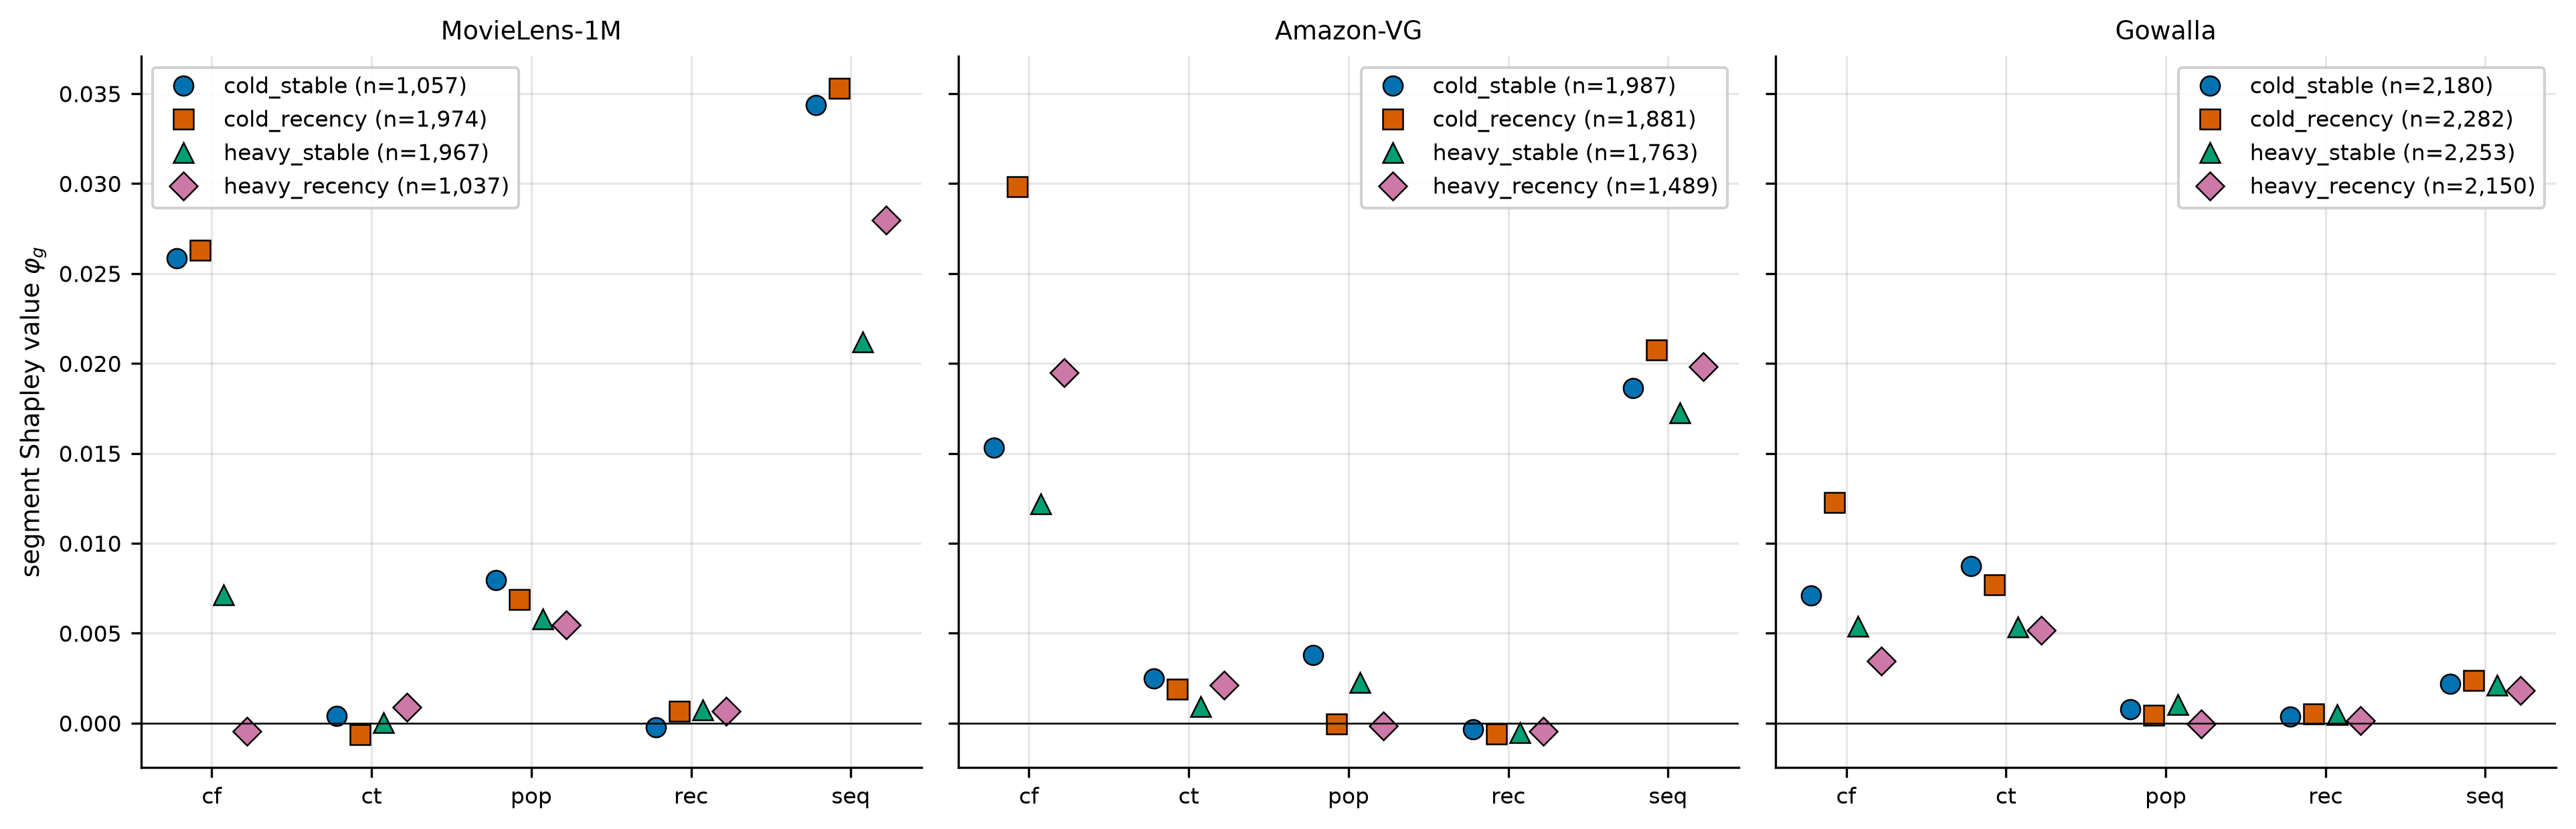
\includegraphics[width=\textwidth]{Fig5.png}
\caption{Descriptive segment-level Shapley values; legends give segment
sizes. No pairwise segment contrast survives within-corpus Holm correction,
so the figure visualises exploratory variation and does not establish
segment-level attribution heterogeneity.}
\label{fig:segments}
\end{figure*}

\paragraph{No cross-corpus omnibus ranking}
A cross-corpus Friedman test would pool absolute $\NDCG$ from two corpora that
fail the declared recall gate and would use only three corpus blocks. We
therefore do not report or interpret an omnibus method ranking; the appendix is
descriptive per corpus.

\paragraph{Fusion weights never see test outcomes}
Because the characteristic function of Section~\ref{sec:game} is evaluated on
test interactions, deriving fusion weights from those same attributions would
be circular. We avoid this: the fusion heads, the segment-specific weights, the
choice of head family, and the shrinkage strength are all fitted on the
\emph{validation} fold only, and are frozen before a single test evaluation.
The Shapley values reported in Section~\ref{sec:results} are diagnostic output;
they are not inputs to the weights.

\paragraph{Attribution-derived fusion gives no resolvable gain over the matched head}
On the MovieLens illustration, weights derived from segment-level attributions
are numerically above uniform fusion
($+0.0118$, $d_z = 0.097$), a popularity reference ($+0.0452$,
$d_z = 0.232$), LightGCN~\citep{he2020lightgcn} ($+0.0295$, $d_z = 0.157$), and
SASRec~\citep{kang2018sasrec} ($+0.0464$, $d_z = 0.243$), at
$\NDCG = 0.06348$ (Figure~\ref{fig:fusion}). These are descriptive differences,
not superiority tests: users share fitted models, the neural references received
smaller tuning budgets, and every effect size is below $0.25$.

Against a globally tuned head of the same family ($\NDCG = 0.06357$) the
attribution-derived head is $0.00009$ \emph{lower} ($d_z = -0.007$,
Holm-corrected $p = 0.23$), which is practically negligible and, in this run,
negative. Under the legacy candidate rule the same comparison came out at
$+0.00003$: the difference is not stable in sign across the candidate
construction, and it is not stable under the plausible per-user normalisation
in Eq.~\eqref{eq:head} either, while its magnitude stays within noise
throughout. A quantity whose sign depends on the truncation key is not
evidence of an advantage in either direction. \textbf{We therefore make no claim
of any advantage over a well-tuned global head}, and note that the comparisons
against LightGCN and SASRec are conditional on tuning budgets that were not
matched to our own pipeline.

\begin{figure*}[tp]
\centering
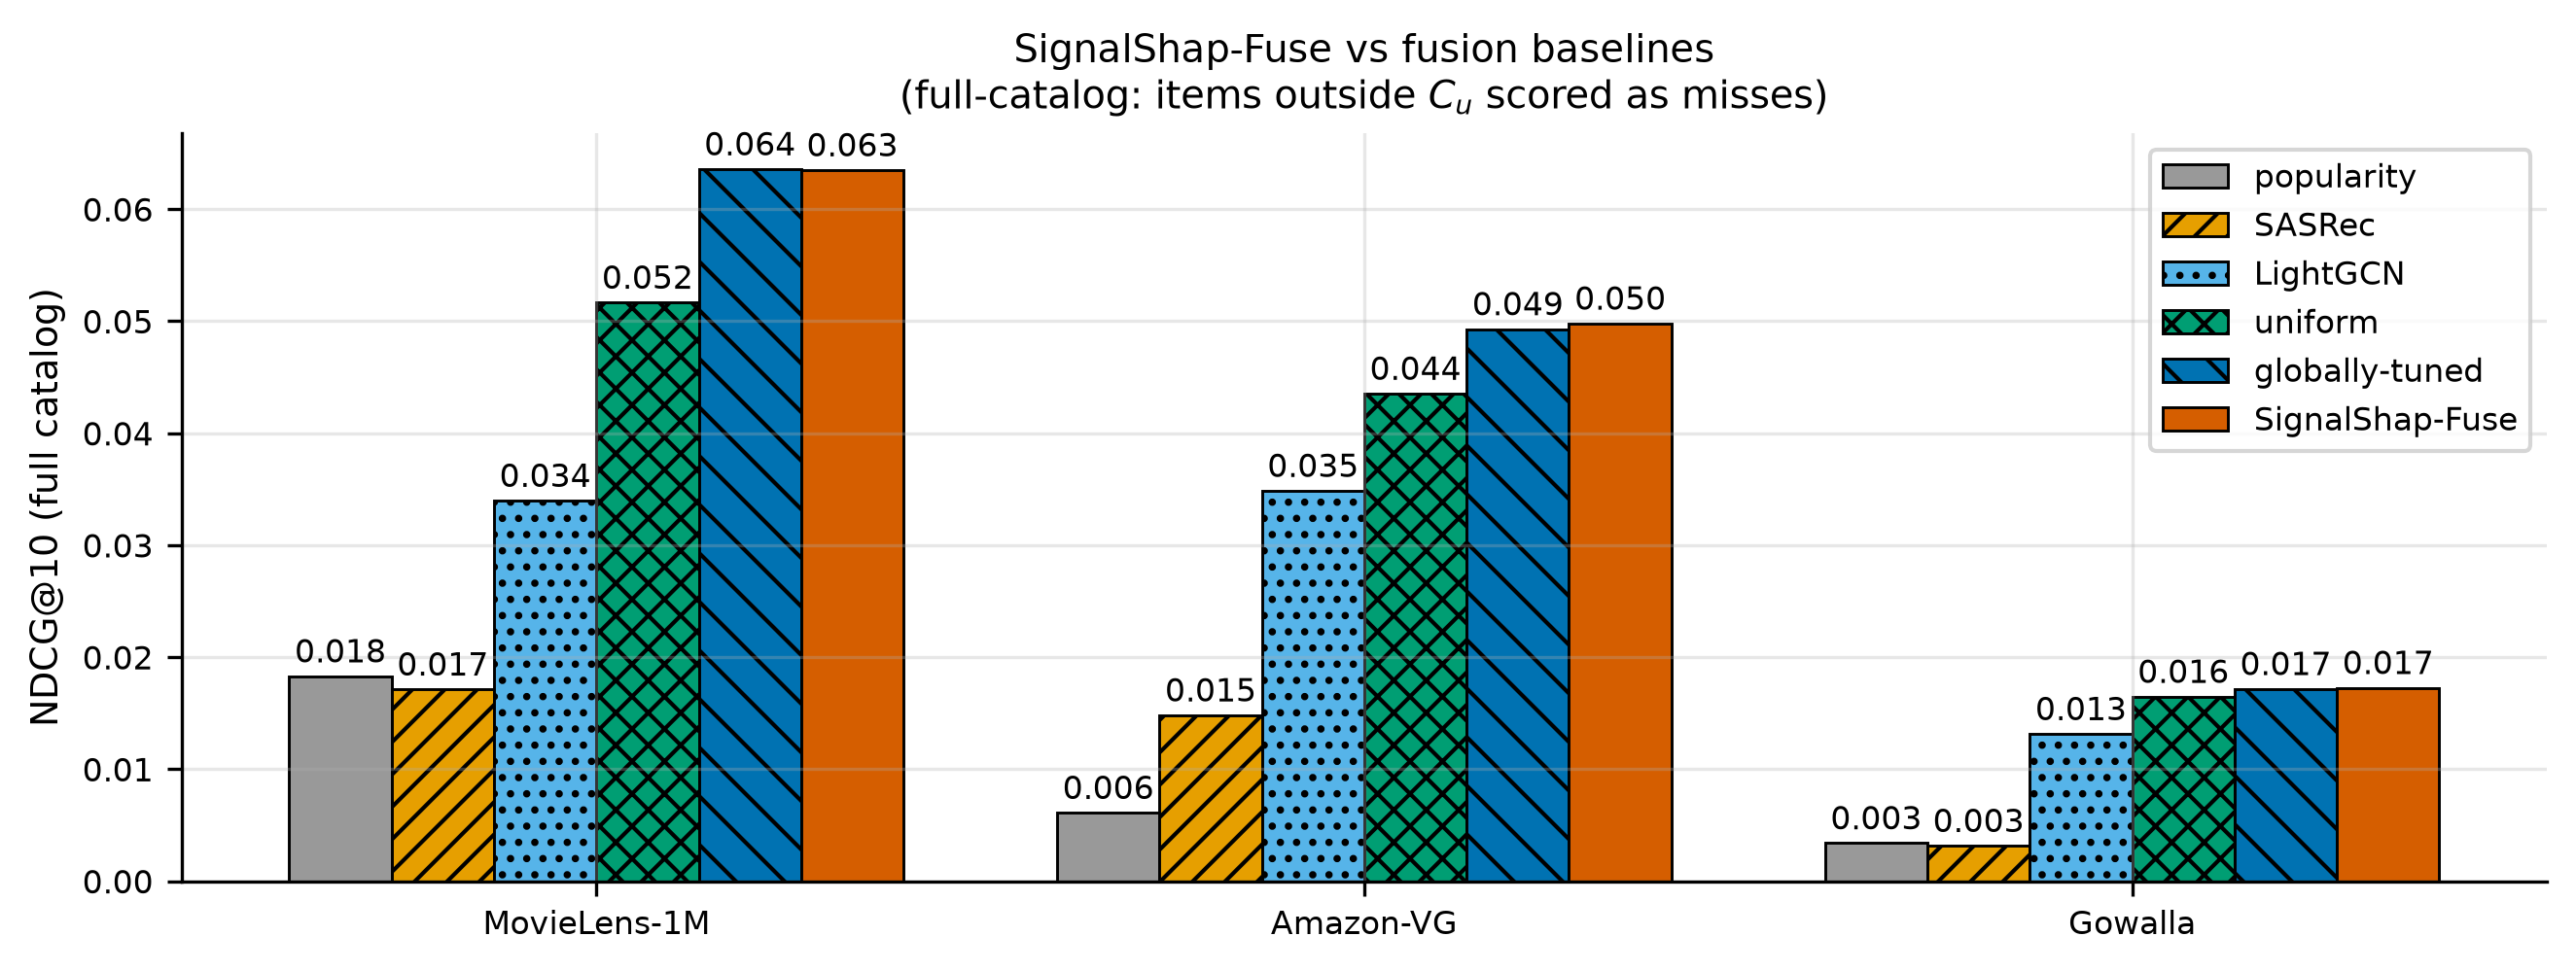
\includegraphics[width=0.85\textwidth]{Fig6.png}
\caption{Full-catalogue fusion comparison; Amazon-VG and Gowalla remain below
the candidate-recall gate.}
\label{fig:fusion}
\end{figure*}

An exploratory bootstrap that resamples seeds and then users within each seed
gives a mean difference of $+0.00005$ with interval
$[-0.00022,+0.00032]$. Because the same users occur under every seed, that
nested procedure does not preserve the crossed pairing and is not used for a
positive equivalence claim. A confirmatory equivalence analysis would require a
multiway or pairing-preserving bootstrap, a prespecified equivalence margin, a
$90\%$ interval, and both one-sided statistics. The defensible conclusion is
narrower: no advantage over the matched global head is resolved in these data.

The contribution stands on the implementation checks of Section~\ref{sec:recovery} and the
attribution results of Section~\ref{sec:results}. This appendix is a negative
result about one downstream use of the attributions, and it is not evidence
either for or against their correctness.

\section*{CRediT authorship contribution statement}
\textbf{Mouad Louhichi:} Conceptualization, Methodology, Software, Formal
analysis, Investigation, Writing -- original draft, Visualization.
\textbf{Redwane Nesmaoui:} Software, Validation, Data curation, Writing --
review and editing. \textbf{Mohamed Lazaar:} Supervision, Methodology,
Resources, Writing -- review and editing.

\section*{Declaration of competing interest}
The authors declare that they have no known competing financial interests or
personal relationships that could have appeared to influence the work reported
in this paper.

\section*{Data availability}
This work uses three public corpora and redistributes none of them.
MovieLens-1M is used under the GroupLens research-use license, Gowalla
check-ins come from the SNAP collection, and the Video Games category is taken
from the Amazon Reviews 2023 corpus; the fetch scripts in the repository
retrieve each from its original source. The corpora themselves are not
redistributed because the GroupLens license forbids it. All derived data
behind every reported number is released with the code, together with
\texttt{MANIFEST.json}, which records a SHA-256 for each artefact file with the
commit and environment that produced it, including the BLAS backend, because
Section~\ref{sec:threats} shows the backend changes candidate contents for a
small number of users. \texttt{PROVENANCE.md} maps every table and figure to
the artefact, platform, candidate rule and seeds behind it. We state the
residual limitation precisely: a reader reproducing from raw data must refetch
the corpora first, and a run on a different BLAS reproduces the reported signs
and orderings but not every fifth decimal.

\section*{Code availability}
The implementation, configuration files, and scripts required to reproduce the
reported experiments, tables, and figures are publicly available at
\url{https://github.com/mouadlouhichi/signalshap}. The results in this
manuscript correspond to repository commit
\path{0b8e998a13610932cef79b8ccb3fab55074263d3}, released as tag
\texttt{kbs-submission}; that commit is the one recorded inside
\texttt{MANIFEST.json} alongside the SHA-256 of every artefact, so a reader can
confirm that the released hashes and the reported numbers come from the same
state of the code.

\section*{Ethics}
The study performs secondary analysis of previously released, de-identified
human-generated ratings, reviews, and check-ins under the dataset licenses
recorded in the artefact, and involves no new participant recruitment or
intervention. Geographic check-ins can retain re-identification risk even after
direct identifiers are removed; we use only aggregate geographic cells and
redistribute no event records. Popularity-based signals can reinforce exposure
disparities, and no fairness claim is made.

\section*{Funding}
The authors declare that no funds, grants, or other support were received
during the preparation of this manuscript.

\section*{Declaration of generative AI and AI-assisted technologies in the
manuscript preparation process}
During the preparation of this work, the authors used OpenAI Codex for code
scaffolding, editorial review, and consistency checking. After using this tool,
the authors reviewed and edited the content as needed and take full
responsibility for the content of the publication.

\bibliographystyle{elsarticle-num}
\bibliography{paper}

\end{document}
